% !TEX program = lualatex
% !BIB program = biber
% Template for authors
%
% Structure:
% ├── acknowledgements.tex: acknowledgements and/or funding information
% ├── authors.tex: authors and affiliations
% └── references.bib: bibliography
%
%
\documentclass{bausteinefdm}
%
%
% The documentclass already loads a number of packages, amongst others:
% - amsmath,amssym
% - xcolor, graphicx
% - babel, csquotes
% - biblatex
% - fontspec, microtype
% - booktabs, longtable
% - listings
\usepackage{todonotes}
\usepackage[nolist,nohyperlinks]{acronym}
\usepackage{tabularx}
\usepackage{subcaption}
\usepackage{enumerate}
\usepackage{enumitem}
%\usepackage[super]{nth}
\usepackage{afterpage}
\usepackage{placeins} % preamble
\usepackage{makecell}
%
% -----------------------------------------------

\makeatletter
\newcommand{\tablelabel}[2]{% \speciallabel{<stuff>}{<label>}
  \edef\@currentlabel{#1}\label{#2}%
}
\makeatother


% \finalfalse
%
%
% To be changed by the editor. Switches between the preprint version (\finalfalse) and the final version (\finaltrue) of the template.

\title{PRO Research Process 4Ing: Project- and RDM-Oriented\\ Research Process for Engineering Sciences}
\subtitle{Validation of a Newly Prosed Process to Combine Data Life Cycles and Project-Oriented Research Processes in Engineering Sciences}

%
% The information on authors and
% affiliations have to be provided in the file: authors.tex
\corresponding{\printcorrespondingauthor}
%
%
% Thanks and acknowledgements  and funding
% information have to be saved in: acknowledgements.tex
%
%


\addbibresource{references.bib}
%
%
% Save all your references in this Bib(La)TeX file
%
%


\begin{document}
\maketitle
\begin{abstract}
% 1.Sentence: Context, 
In a first paper \cite{Hamann.2024b}, we have shown the absence as well as the importance of a project-oriented \hyperref[Glossary:research data management level]{\ac{rdm}} process for engineering sciences.
% 2.Sentence: Importance of Research
We argue that the integration of \hyperref[Glossary:research data management level]{\ac{rdm}} into the practice would greatly benefit by the availability of such project-oriented \hyperref[Glossary:research data management level]{\ac{rdm}} process.
% 3.Confrontation/Research gap,
While many \hyperref[Glossary:research data management level]{\ac{rdm}} and engineering research processes already exist, a combination of both was only recently designed in our previous paper \cite{Hamann.2024b}.
% 4.Exact Research Question
Seeking for validity of the proposed RDM process, the research question in this article is: \enquote{Can our proposed \hyperref[Glossary:research data management level]{\ac{rdm}} process be deployed into engineering research projects?}
% 5.Resultion: Method applied,
We interviewed ten (n=10) experts on their research practices and the fit of the proposed process to their research activities.
% 6.Solution of the Method,
Overall, we found a broad acceptance of the proposed process, as well as several possible potentials for enhancements, e.g. regarding wording and loops.
% 7.Main Contribution done 
As a result, this paper presents a validated project-oriented \hyperref[Glossary:research data management level]{\ac{rdm}} process for engineering sciences.
\end{abstract}

\linenumbers


\section{Introduction}
\label{Introduction}
%\todo[color=red]{@TH: Prozessnamen in Intro und Conclusion}
% Brief motivation
Integrating \hyperref[Glossary:research data management level]{\ac{rdm}} processes into day-to-day work is still a hurdle for researchers in engineering sciences. \cite{Wuchner.2023, Ortloff.2023}
We showed the reasons for that in our previously published paper 
\textit{Matching Data Life Cycle and Research Processes in Engineering Sciences}
\cite{Hamann.2024b}: %HAMA24d:
While many suggestions on how to carry out \hyperref[Glossary:research data management level]{\ac{rdm}} already exist \cite{ELIXIRCONVERGE.2023, Politze.2019, Higgins.2008}, 
their integration into practice is not feasible on a one-to-one basis focusing on a strong theoretical reference \cite{Cox.2018}.
In this context, the \ac{dlc} model is often used to refer to only \ref{Glossary:research data}. However, it cannot be transferred to research activities in general, yet it is frequently used for this purpose \cite{Hamann.2024b,Cox.2018}.
Furthermore, for engineering sciences, \ref{Glossary:project}-orientation and specificity in engineering are missing in \hyperref[Glossary:research data management level]{\ac{rdm}} processes. \hyperref[Glossary:project]{Project}-oriented research has been increasing rapidly for years 
\cite{Krull.2016, Winterhager.2015,Bonn.2009,Berning.2005}, which is enforced by the \enquote{greater third-party funding activity in the natural sciences and engineering} \cite{Berning.2005}.
This \ref{Glossary:project}-oriented approach spans through all forms of research and occurs in basic research as well as in applied research. \cite{Behlau.2017}


% gap statement
In our first paper \cite{Hamann.2024b}, we addressed this challenge (lack of integration of \hyperref[Glossary:research data management level]{\ac{rdm}} into day-to-day work and \ref{Glossary:project} structures) while also focussing on the demands of researchers in engineering sciences. 
%\subsection{Identified research gap}
%\label{Gap}
By that we identified two main issues with the state of the art in \ref{Glossary:project}-oriented \hyperref[Glossary:research data management level]{\ac{rdm}} processes.
First, while the variations of detail and complexity in the processes as well as the definition of their sub-steps and activities are vast, there is not yet a process with a scope, that reaches from the \ref{Glossary:project} as a whole down to the data in detail.

Second, there is a gap between \ac{dlc}s and other, more holistic models. \cite{Hamann.2024b} %HAMA24d
While \acp{dlc} support the management of data along its life cycle, they are not supposed to be utilised as a support structure for \ref{Glossary:project} management.
\acp{dlc} are a \enquote{useful metaphor, but tend to encourage thinking that research processes are highly purposive, uni-directional, serial and occurring in a closed system. Research is often not like this} \cite{Cox.2018}.
Contrasting this insufficiency, engineering research processes often lack \hyperref[Glossary:research data management level]{\ac{rdm}} context and applicability.
Hence, a process combining both \ref{Glossary:project}-oriented research and \hyperref[Glossary:research data management level]{\ac{rdm}} did not exist to the best of our knowledge.
We aimed to close this gap with our proposed process.


The \ref{Glossary:finding} of this first paper \cite{Hamann.2024b}  is a multi-layered \hyperref[Glossary:research data management level]{\ac{rdm}} process, combining the overall structure of \ref{Glossary:project}-oriented research with the \ref{Glossary:execution} of research and the handling of data as depicted in figure \ref{fig:Levels}.

\begin{figure}[ht]
    \centering
    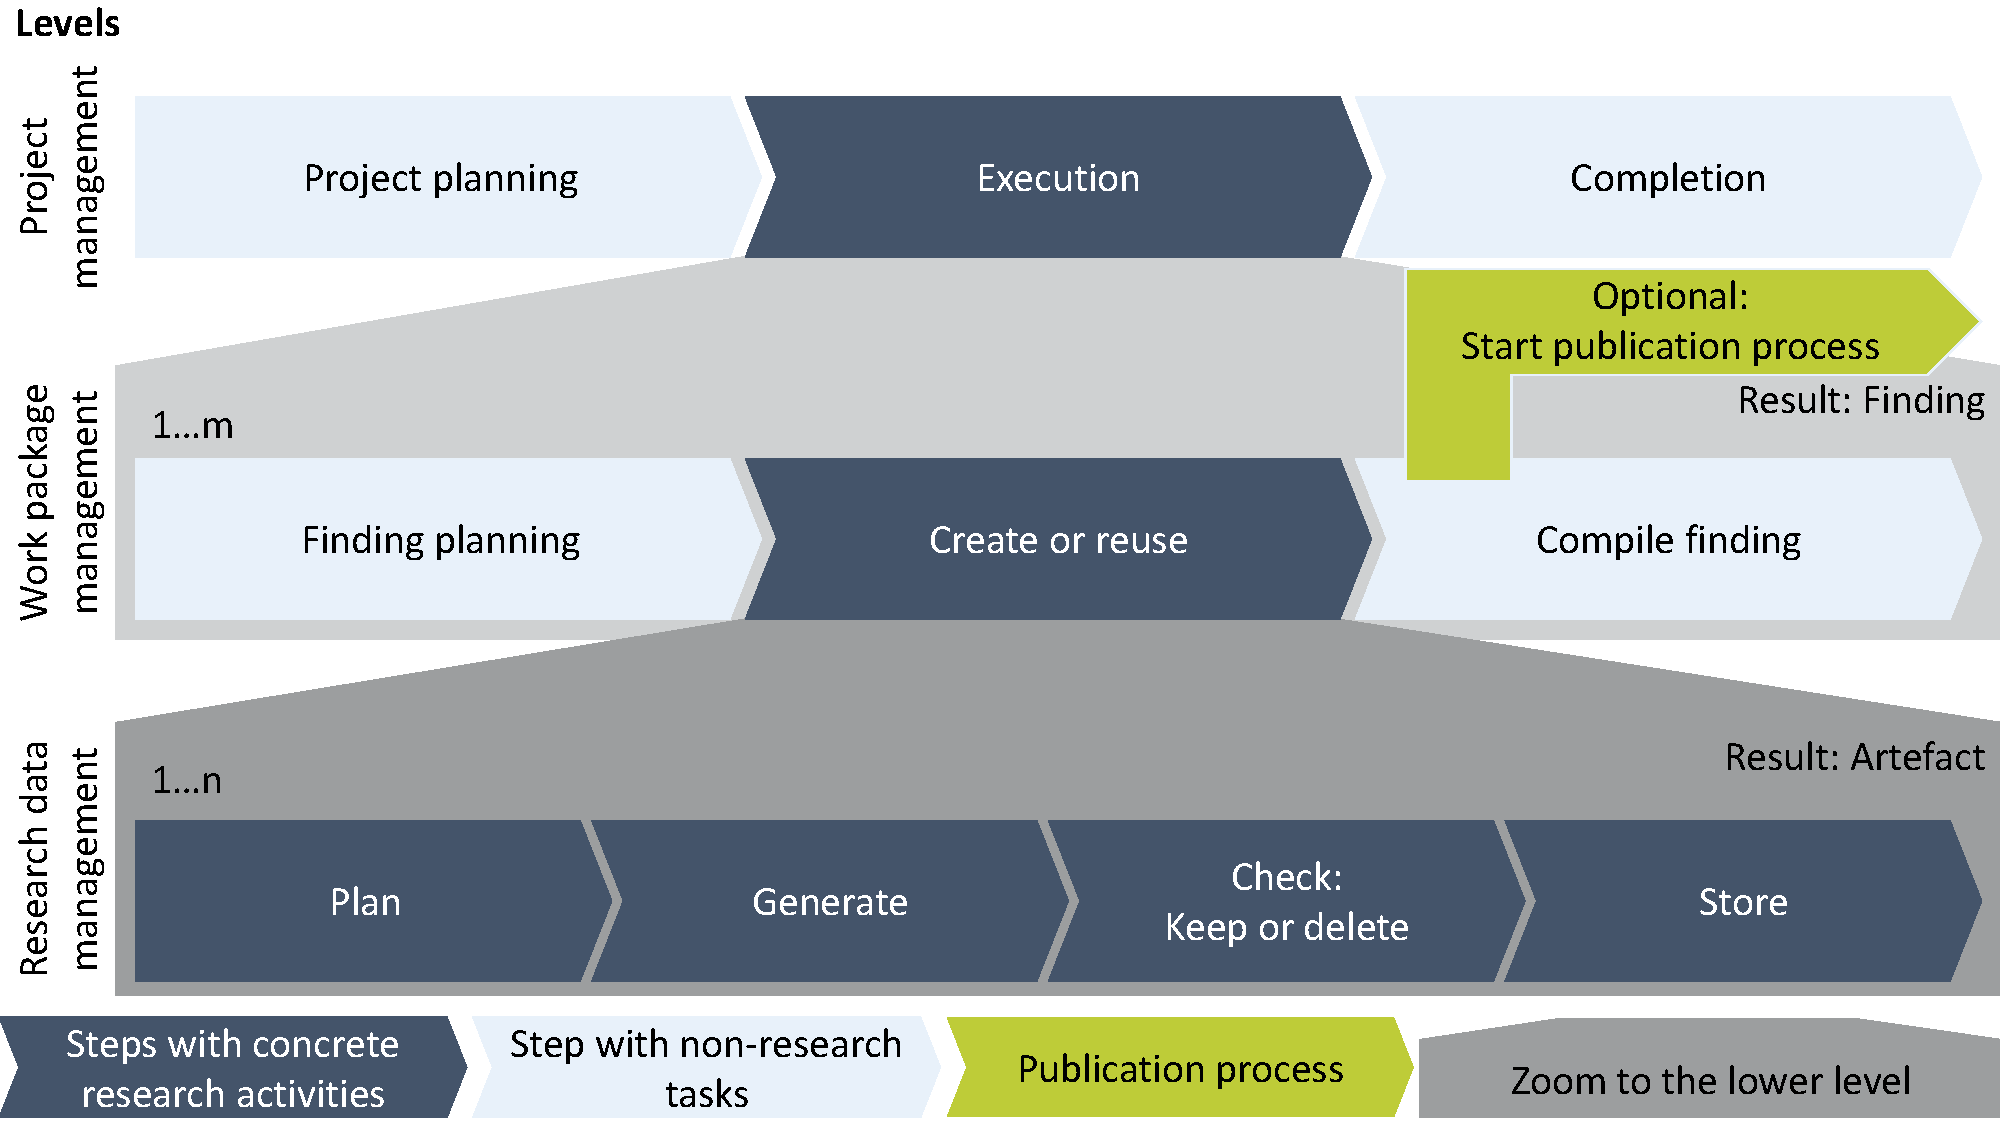
\includegraphics[trim={0 0.2cm 0cm 0cm}, clip, width=\textwidth]{figures/Levels_v2.pdf}
    \caption{General structure of the previously designed \hyperref[Glossary:research data management level]{\ac{rdm}} process \cite{Hamann.2024b}}
    \label{fig:Levels}
\end{figure}

On the highest level, the \textbf{\ref{Glossary:project management level}}, waterfall-like approach divides the research project into three phases.
In the second phase, the \ref{Glossary:execution}, the actual research takes place in form of the \ref{Glossary:content-wise execution}.
Within this \ref{Glossary:content-wise execution} the lowest level of research is found, where data collection is planned, conducted, checked for sanity and the data is stored for further use.
This lowest level of research resembles the concept of \acp{dlc} and creates an \ref{Glossary:artefact}.
One or more artefacts can be compiled to a \ref{Glossary:finding} to answer a research question or complete a work package of a research project.
One or more findings will lead to the goal of the project.
For further detail on the process, please refer to appendix \ref{PreviousProcess} or our first paper \cite{Hamann.2024b}.


While this process was built upon two data collections of researchers' practices and demands, the resulting process has to be cross-checked by its users to ensure that it is sufficient in filling the identified gap.
On this basis, the applicability of the process has to be evaluated and validated in this article, leading to the research question:

\hfill\begin{minipage}{\dimexpr\textwidth-0.5cm}
    \textit{
    \textbf{Can our proposed \hyperref[Glossary:research data management level]{\ac{rdm}} process be deployed into engineering research projects?}}
\end{minipage}

To answer the proposed research question, we conducted ten qualitative expert interviews.
Experts were questioned on their day-to-day research activities and the fit of the proposed process \textendash{} later called \ac{prorp} \textendash{} to these activities. 
It has to be mentioned that this article only describes the validation of the process itself as an \enquote{artificial evaluation} \cite{Venable.2006} to prove its fit to the proposed field of engineering sciences.
The validation of the framework that inherits this process in a real world application was conducted by Hamann et al. \cite{Hamann.2025b} in a Proof-of-Concept-Study.

The further structure of this paper is divided into four sections.
%follows the line of reasoning in the \hyperref[Introduction]{introduction}.
Firstly, in section \ref{Research methodology} we 
%sketch out \hyperref[Related work]{related work} and present the \hyperref[Gap]{identified research gap}.
elucidate the \hyperref[Research methodology]{research methodology} used to validate and enhance our process.
Secondly, the results of the validation are shown in section \ref{Results}, which describes the collected feedback to the \hyperref[PreviousProcess]{previously designed process} for the possible enhancements.
After that, section \ref{Discussion} discusses the methodology and limitations of the validation.
Lastly, the paper closes with a \hyperref[Discussion]{conclusion and discussion} (section \ref{Conclusion and Outlook}).

%\section{Related work and existing research gap}
%\label{Related work}






\section{Research methodology} 
\label{Research methodology}

To answer the proposed research question, we conducted expert interviews and analysed using qualitative content analysis.
We conducted ten interviews, transcribed, anonymised, coded and aggregated.
In the following, the exact procedure is explained.

\subsection{Collecting the data: Planning and conducting the interviews}
\label{Interviews}
%\todo[inline]{Methode nach Gläser}
Expert interviews were conducted to validate the process. 
Interviews in general are a qualitative method of data collection that originates from the social sciences. \cite{Bogner.2009b, Froschauer.2009}
The question posed was processed using non-standardised interviews - more precisely, guided interviews. 
In this approach, interviewers use a guideline that complies topics and questions they are expected to introduce during the interview. 
In order to create a natural flow of conversation, they can use the guidelines flexibly, adapt the order of questions and ask follow-up questions. 
This should allow the interviewees to answer as freely as possible. 
The expert interview method was chosen because a special type of knowledge was required for the validation: 
not only specialised knowledge, but also practical knowledge. 
In this type of interview, the experts themselves are not the object of investigation, but the medium through which the information for answering a question is collected. \cite{Glaser.2010}
The guideline for the expert interviews has been designed following the remarks of Gläser and Laudel \cite{Glaser.2010}.

%\todo[inline]{Geplante Teilnehmende}

Our goal was to have at least one interviewee - resp. expert - per \ac{tu9}-university, the Alliance of leading Universities of Technology in Germany, representative of engineering research at universities in Germany. 
In order to find experts who actually have the type of knowledge required, there were requirements for the interviewees: 
As the proposed process focusses mainly on engineering sciences, researchers had to have a corresponding engineering background.
Furthermore, we demanded at least four years of experience in research.
After some enquire, we could reach our goal of one interviewee per \ac{tu9}-university with the required background.

%\todo[inline]{Leitfaden}

The created interview guideline contained five parts (see table \ref{tab:InterviewGuideline}).

%\newcolumntype{b}{X}
\newcolumntype{s}{>{\hsize=.3\hsize}X}
\begin{table}[ht]
    \begin{tabularx}{\textwidth}{s|X}
        % \toprule
        \textbf{Part of the guideline} & \textbf{Content of the part} \\
             \toprule
         Part 1: Experiences with RDM & Previous experiences and attitudes towards RDM to contextualise the answers\\
         \midrule
         Part 2: Presentation of the process & Interviewees were allowed to ask questions about the process and clarify ambiguities before the discussion \\
         \midrule
         Part 3: Survey on the fit of the process to the interviewees' own research & Interviewees outlined the example \ref{Glossary:project} and were asked about the fit in this \ref{Glossary:project} for each process level as well as the \ref{Glossary:publication process} and the overall process. They first freely described how the research was conducted, after which the process was shown and they were asked for concrete comparisons to their descriptions. \\
         \midrule
        Part 4: Information on the interviewees & A few demographic questions about the interviewees' careers and specialised contexts \\
        \midrule
        Part 5: Conclusion & Space for concluding remarks and questions as well as an outlook on the further validation process \\
            % \hline \hline
        % &&            Sum: & \\
        % \bottomrule
    \end{tabularx}
    \caption{Structure of the interview guideline}
    \label{tab:InterviewGuideline}
\end{table}

The free descriptions of their research activities were intended to ensure that the interviewees did not orientate themselves to the process before the interviewers asked for direct comparisons. In this way, the actual state was queried and not implicitly associated with a target state. Nevertheless, it was necessary to make the process accessible to them before the interview so that they could prepare themselves.
The demographic section (part 4) asks respondents to categorise their technical and professional situation so that their answers can be put into context.

%\todo[inline]{Review und Pretest}
This guideline was reviewed by an expert for survey methods form the \ac{wzl-iqs-en} at the \ac{rwth} and adapted accordingly.
Additionally, a pretest was performed with a researcher from the \ac{rwth}.
The learnings of the pretest were considered when conducting further interviews: minor improvements in the technical setup, interviewer behaviour trough gaining experience, minor changes in the wording of questions.
However, as these learnings were not focussed at the core content of the guideline, the pretest was still considered usable and was also included into the final results.

%\todo[inline]{Vorbereitung der Teilnehmenden und Durchführung}

The interviewees received for preparation an introduction to the interview and the declaration of consent to the interview as well as a description of our proposed \hyperref[Glossary:research data management level]{\ac{rdm}} process in form of an excerpt from the previous article about it \cite{Hamann.2024b}. They were asked to sign the declaration of consent, read the article and to think about a \ref{Glossary:research project} in which they were involved, ideally from the application phase to the \ref{Glossary:project completion}. If they were not involved in a \ref{Glossary:research project} from start to finish, they were supposed to choose a \ref{Glossary:research project} in which they were involved for as long as possible and in which they experienced either the application phase or the \ref{Glossary:project completion}.

The interviews lasted approximately one and a half hours each and were conducted by two interviewers simultaneously, one researcher and one member of the research supporting staff. This made it possible to divide the interviews according to background knowledge and to ask differentiated questions. The interviews were conducted online and recorded.
% \todo[color=green]{Optionales To do: Leitfaden online stellen}

\subsection{Preparing the data: anonymization and stock of data}
\label{AnonymisierungDatenbestand}

%\todo[inline]{Anonymisierung}

After each interview, the recording was transcribed with the support of a custom python pipeline for audio transcription.
The transcription was anonymised partly automated using QualiAnon\footnote{\url{https://github.com/pangaea-data-publisher/qualianon}}. \cite{Mozygemba.2023}
Afterwards, the anonymised transcripts were imported into MaxQDA\footnote{\url{https://www.maxqda.com/}}.

%\todo[inline]{Datenbestand: Demographie, Porjekte etc., s. auch 4.1?}

Ten interviews were included in the subsequent analysis: one from each of the TU9 Universities and the pretest at RWTH Aachen University.
The interviews contain a total of 117,066 words.%\todo{Notiz an MR: Aufhänger für LinkedIn: "117066 Wörter braucht es, um einen Prozess zu evaluiseren."}

The demographic questions make it possible to categorise the interviewees in terms of their technical and professional backgrounds: 
The interviewees' scientific carriers are mostly set in mechanical engineering, but also in industrial engineering and economics. 
Data science and civil engineering are also represented. 
This means that the engineering sciences are thematically diverse in the interviews, which increases the quality of the validation.
The interviewees already have a doctorate degree or are about to complete it. 
They have experience as research assistants, but also in research and transfer management. 
Some also fulfil management roles such as \ref{Glossary:project} and group leaders. 
Also, one professor was participating in the interviews.
The minimum required four years of professional experience was mostly exceeded, in some cases significantly with eight years or more. 
These professional backgrounds guarantee the availability of the required expert knowledge and enable differentiated perspectives on the process.

All interviewees had already had contact with RDM. Their activities were partly of an administrative nature, partly they had used it themselves - both in solo work while writing their dissertations and in \ref{Glossary:project}s of different sizes. In the discussions, they mentioned many aspects of RDM that they had already encountered: archiving (hardware and software), publication, creating guidelines, Documentation, \ac{dmp}s. They often did not work systematically, but intuitively and according to the "trial and error" principle, because knowledge was often lacking. Due to this lack of knowledge, tools that are not yet fully developed, external and internal guidelines that must be adhered to and poor integration into day-to-day work, their experiences with RDM have so far been predominantly bad. However, there are also interviewees who have had good experiences because they have benefited from the RDM activities after enduring initial stress.

Also, the interviewees were asked to bring an example \ref{Glossary:project} which would function as a mental guideline to describe their research processes.
These \ref{Glossary:project}s were also surveyed in the interviews.
These ranged from very personal \ref{Glossary:project}s with only a single person involved, e.g. doctoral degree \ref{Glossary:project}s, to big scale \ref{Glossary:project}s with multiple institutions involved.
Both \ref{Glossary:project}s with and without industry participation were brought up by the interviewees.
In terms of content, the \ref{Glossary:project}s described ranged from research on artificial intelligence, data modelling and processing, simulation, quality and process management, robotics, circular economy, computational science, manufacturing technology and electronics.\footnote{This categorization was simplified for anonymisation reasons.}

\subsection{Analyse the data: qualitative content analysis}
\label{QualitativeContentAnalysis}

%\todo[inline]{Qualitative Inhaltsanalyse als Methode}
In MaxQDA, the transcripts were analysed based on the qualitative content analysis method as proposed by Mayring \cite{Mayring.2022}. 
Qualitative content analysis analyses material with regard to its content. \cite{Flick.2009}
Since this material represents fixed communication (texts, images, music, etc.), the communication itself is also the subject of the analysis. It is characterised by a systematic, rule- and theory-based approach. The following section describes the practical implementation of this validation.

%\todo[inline]{Umsetzung der Methode, Codestruktur etc.}

Modelled after Mayring \cite{Mayring.2022}, a process adapted to this validation was created as shown in figure \ref{fig:Qualitative_Content_Analysis_Process}:
The code system was formed deductively based on the theory and the question: one code each for agreement and disagreement per level and sub-step (cf. figure \ref{fig:Code-System})  as well as seven other codes, which are listed in table \ref{tab:DescriptiveFeedback}. 

\begin{figure}[ht]
    \centering
    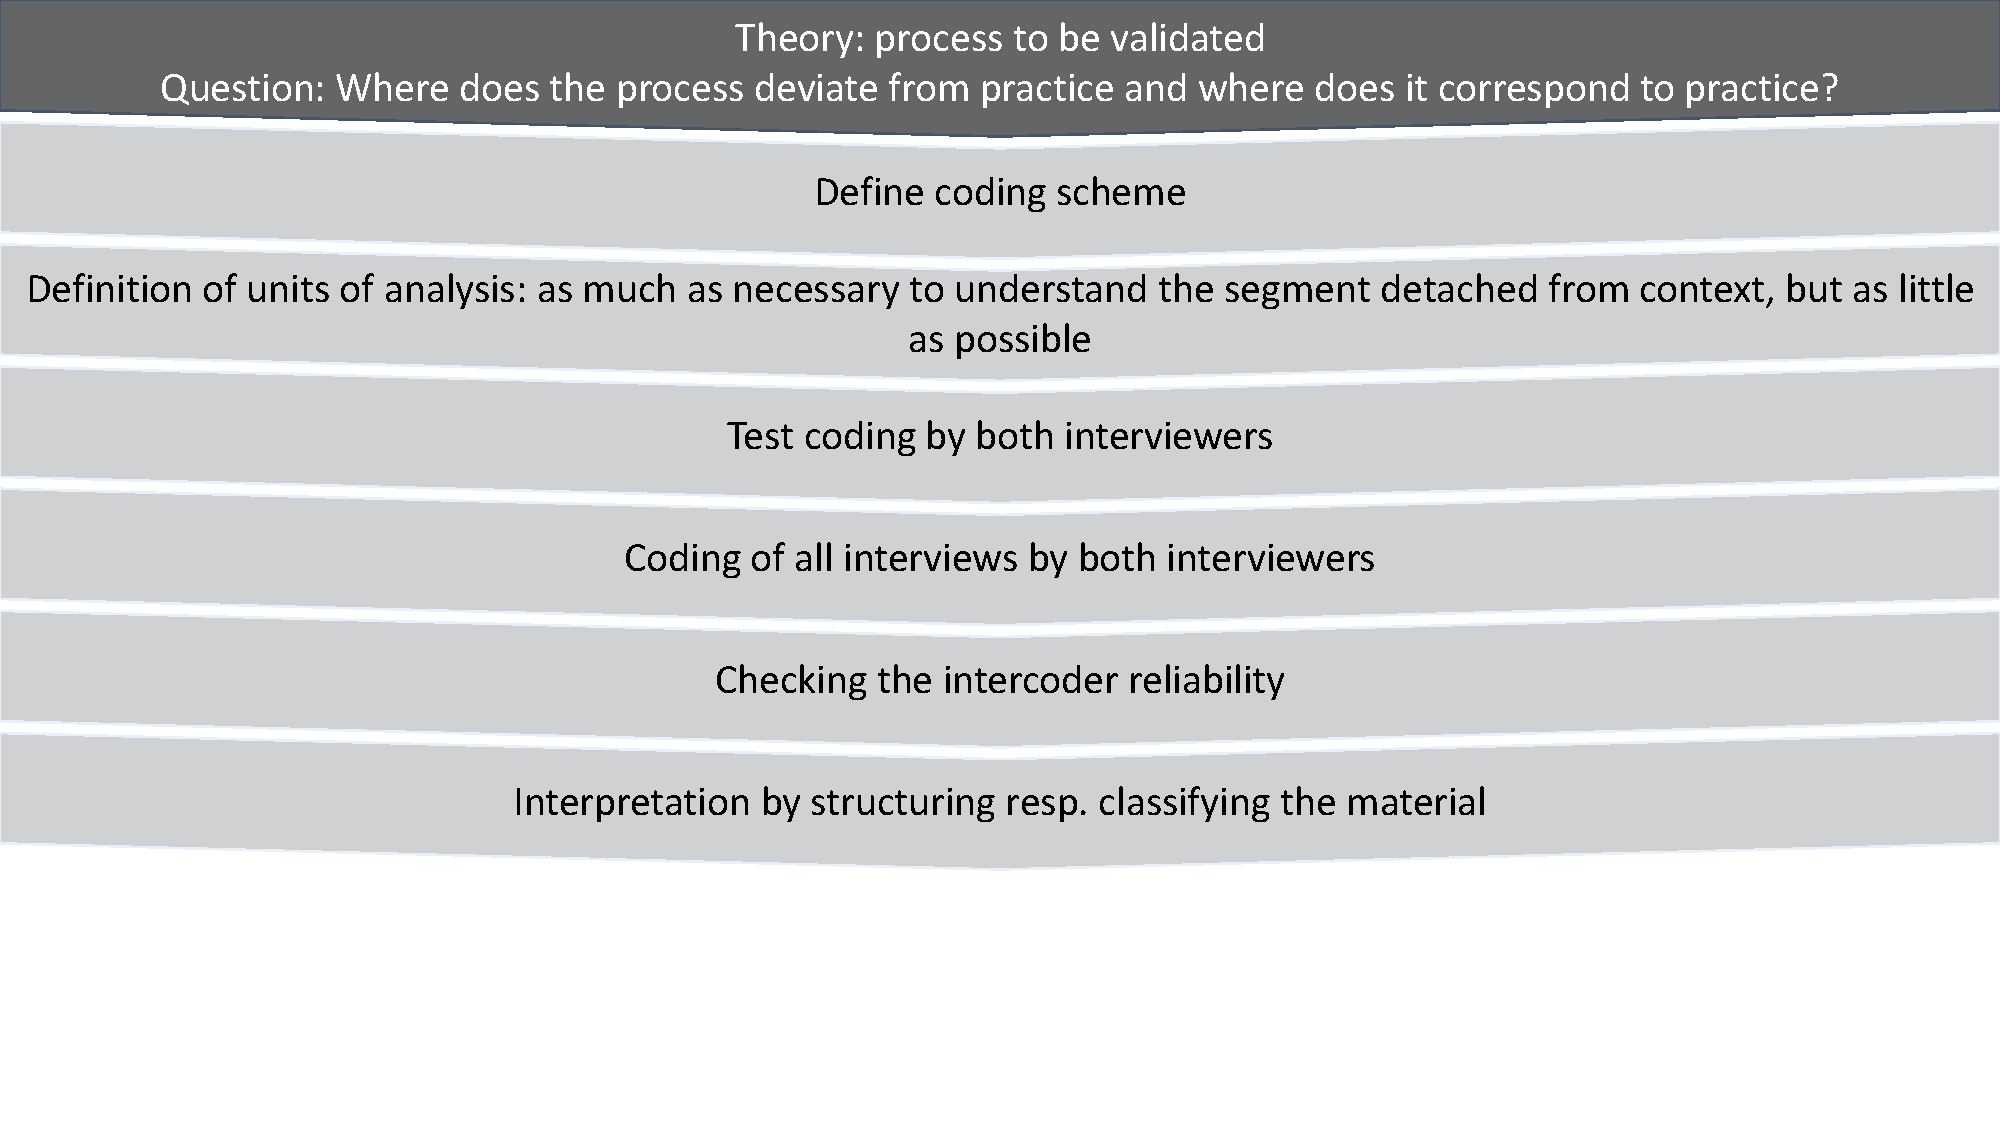
\includegraphics[trim={0 4.5cm 0cm 0cm}, clip, width=\textwidth]{figures/Qualitative_Content_Analysis_Process.pdf}
    \caption{Content-analytical model based on \cite{Mayring.2022}}
    \label{fig:Qualitative_Content_Analysis_Process}
\end{figure}

A total of 66 codes were used, resulting on 741 coded segments in the ten interviews. 
Structuring resp. classification was used as the basic form of interpretation, i.e. filtering out certain aspects from the material by fitting its content into the code system.

\begin{figure}[ht]
    \centering
    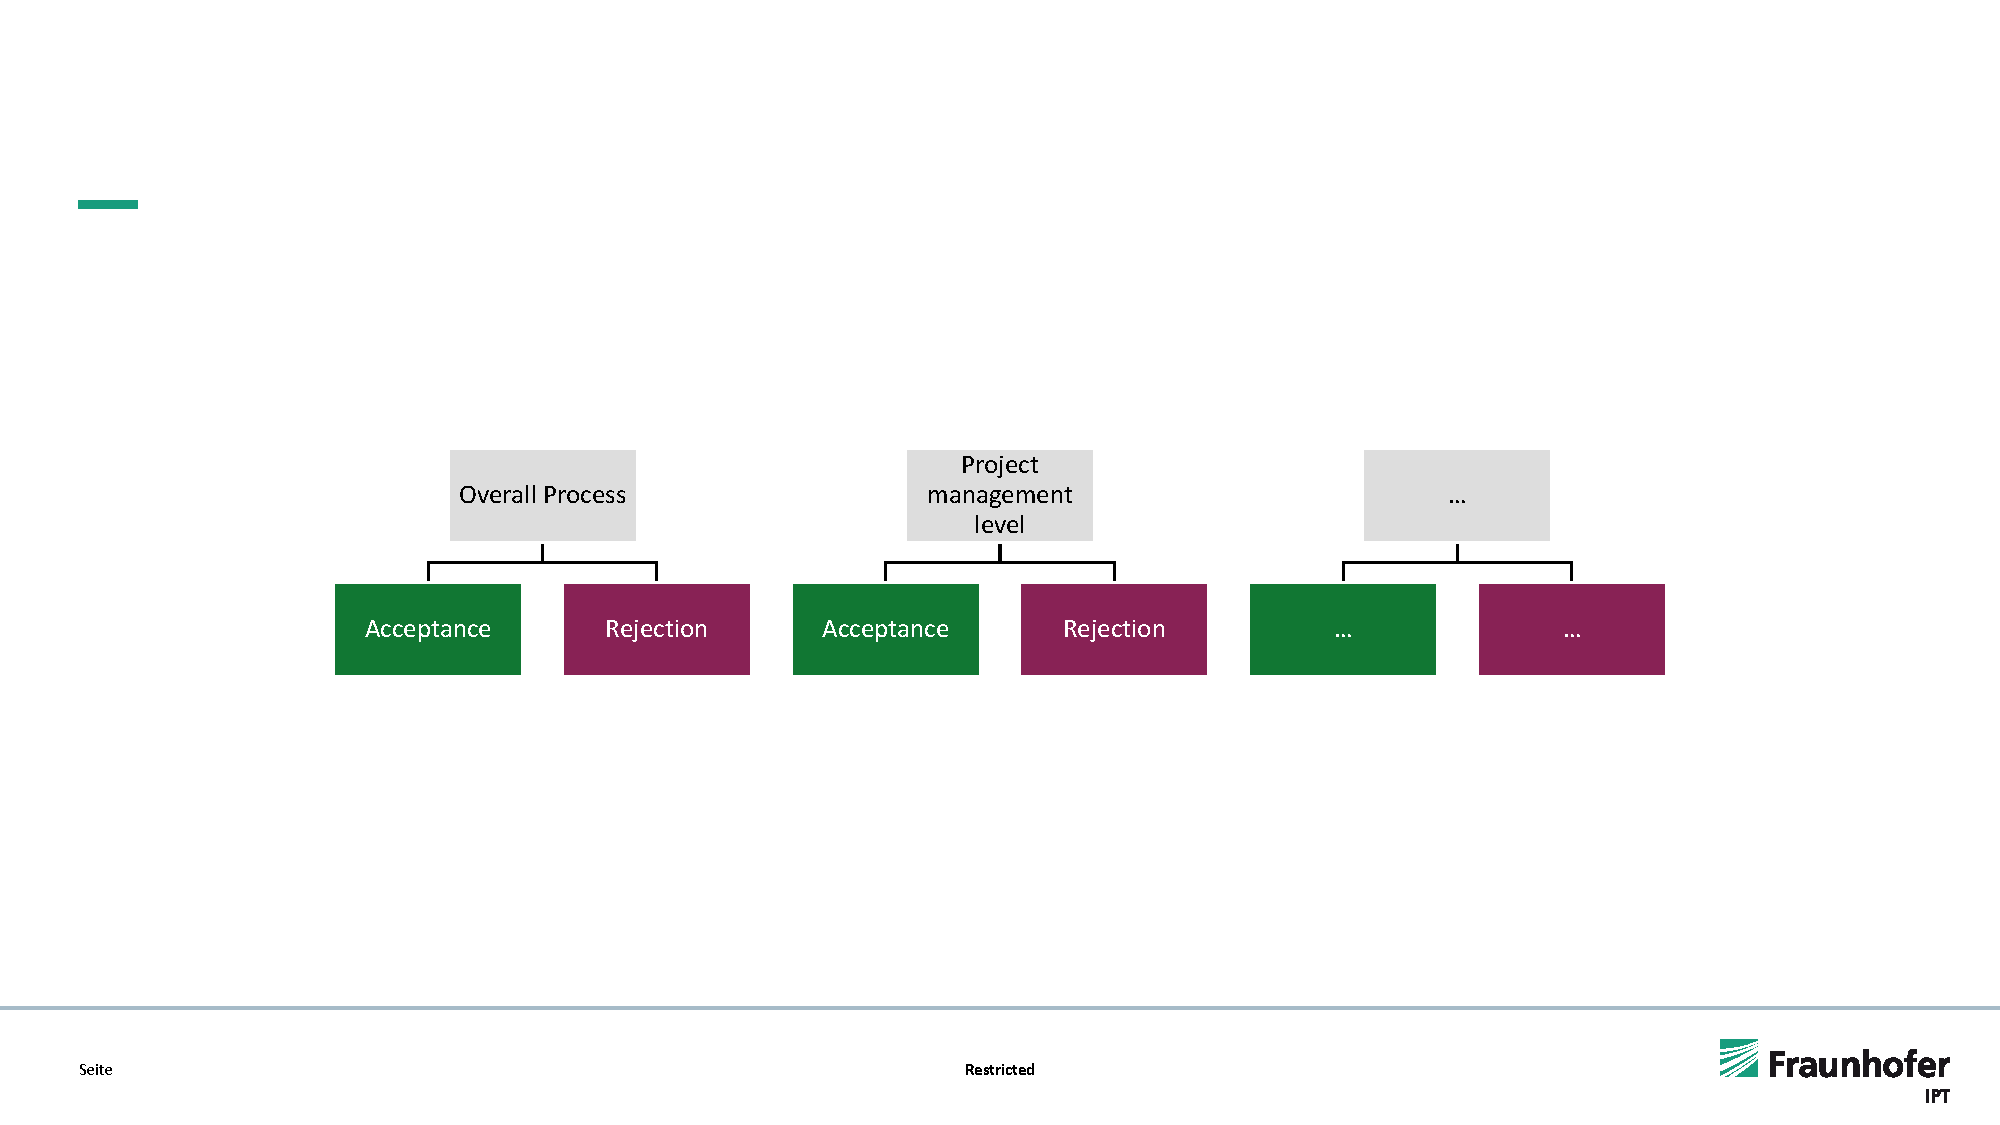
\includegraphics[trim={5cm 7cm 5cm 7cm}, clip, width=1.1\textwidth]{figures/Code-System.pdf}
    \caption{A sketch of the utilised code system}
    \label{fig:Code-System}
\end{figure}

%\todo[inline]{Codes:  71 - Kodierte Segmente: 741 - MR: müssen wir noch mal nachgucken, hatte das einfach rauskopiert. 71 Codes kommt mir doch irgendwie zu viel vor}
%\todo[inline,color=purple]{Michéle: Guck dir mal 4.1 an}
The coding was performed by the two interviewers individually to improve reliability and objectivity.

%\todo[inline]{Interrater reliability}

Afterwards, the codes were reviewed by a lead interviewer, using an intercoder analysis.
In this analysis, similar coding, e.g. same codes with slightly different start and endpoints of the codes, was equalised.
Additionally, conflicting codes, e.g. codes for acceptance and rejection for the same sections of transcripts, were identified.
Conflicts were discussed between the reviewers and solved if possible, e.g. when a wrong coding was accidentally applied.
However, only few conflicts could be solved that way.
The conflicts that could not be solved in that way point towards inconsistencies in the proposed process and therefore show possible improvements.
These inconsistencies and improvements are discussed in the \hyperref[Results]{results and changes to the process}.

%Another interrater reliability analysis was performed on the agreed coding of the transcripts.
%\todo[inline,color=purple]{Michéle bitte ergänzen}

Concluding the analysis, the coded sections were summarised by their respective codes.
In that way, statements to each code could be aggregated.
These aggregations are further condensed into the \hyperref[Results]{results and changes to the process}.%\todo{@MR: Methodenkritik ergänzen}


%\todo[inline]{Forschungsmethodik erklären mit Interviews - Anonymisierung - Codierung - qualitative Inhaltsanalyse (Quelle fügt MR ein) - Demographische Beschreibung der Befragten und Projekte - etc.}






\section{Results and changes to the process}
\label{Results}

In this section, the results are presented. 
Firstly, a \hyperref[DescriptiveFeedback]{descriptive feedback on the interviews} is given.
Afterwards, general feedback on the overall process is presented.
Lastly, the different process levels are discussed regarding their inconsistencies in the proposed process and possible improvements.
The coded segment are referred to as \textit{statements} in the following. 
We have translated German statements into English.

\subsection{Descriptive analysis of the interviews}
\label{DescriptiveFeedback}

The overall feedback given is positive.
More than two thirds of the evaluative statements are expressing acceptance of the process in general or certain parts of it.
The rest of evaluative statements express rejection.
In total, about a third of all statements are indifferent, i.e. they are not giving evaluative statements on the process.
These encompass the demographic descriptions of the interviewees along with their knowledge on \hyperref[Glossary:research data management level]{\ac{rdm}} so far, descriptions of their \ref{Glossary:project}s used as examples, and statements on other topics on \hyperref[Glossary:research data management level]{\ac{rdm}}.
Furthermore, internal annotations were made to point out passages of interest amongst the reviewers.
An overview is given in Table \ref{tab:DescriptiveFeedback}.


\begin{table}[ht]
    \begin{tabularx}{\textwidth}{l|X|X|X||X}
        % \toprule
        \textbf{Code Group} & \textbf{Acceptance} & \textbf{Rejection} & \textbf{Indifference} & \textbf{Total group sum}  \\
        \toprule
        Overall process      & 31 & 7 & 0 & 38 \\
        Project management level  & 92 & 40 & 11 & 143 \\
        Work package management level & 74 & 22 & 8 & 104 \\
        Research data management level & 73 & 28 & 10 & 111 \\
        Publication workflow  & 55 & 46 & 31 & 132 \\
        \midrule
        Other topics (subtotal) & 0 & 0 & 213 & 213 \\
        \midrule
        \, Project description & \, 0 & \, 0 & \, 46 & \, 46 \\
        \, \hyperref[Glossary:research data management level]{\ac{rdm}}-application & \, 0 & \, 0 & \, 27 & \, 27\\
        \, Demographics & \, 0 & \, 0 & \, 23 & \, 23\\
        \, Possible support structures & \, 0 & \, 0 & \, 14 & \, 14\\
        \, Project structures & \, 0 & \, 0 & \, 12 & \, 12\\
        \, Influencing factors & \, 0 & \, 0 & \, 7 & \, 7\\
        \, Others & \, 0 & \, 0 & \, 16 & \, 16\\
        \, Internal annotations & \, 0 & \, 0 & \, 68 & \, 68\\
        % \hline \hline
        % &&            Sum: & \\
        \bottomrule
        \bottomrule
        \textbf{Total sum}  & 325 & 143 & 273 & 741 \\
        \textbf{Total sum percentages}  & 43.9\% & 19.3\% & 36.8\% & 100\% \\
    \end{tabularx}
    \caption{Codes on the feedback received}
    \label{tab:DescriptiveFeedback}
\end{table}

\subsection{General feedback on the process}
\label{GeneralFeedback}

% \todo[inline]{Ingenieure brechen probleme immer auf teilsysteme herrunter}
The general perception of the process is very positive.
31 of 38 statements, or 81.6\%, of the interviewees are positive about the fit of the process to their day-to-day work.
One consensus by the interviewees was the positivity about how the structure of the process is set up from the whole \ref{Glossary:project} to the smallest units of research.
The division of complex problems into smaller parts is inherent to engineering sciences.
One statement in particular summarised this:

\hfill\begin{minipage}{\dimexpr\textwidth-0.5cm}
    \textit{
        \enquote{
            In other words, we try to break this task down into smaller subtasks. (...) This often works relatively well because this entire engineering structure is actually organised in this way. In other words, when we look at a system, I can actually always break this system down further into smaller subsystems with corresponding system boundaries etc. and actually go deeper, deeper, deeper until I just have a single element.% Das heißt, wir versuchen eben diese Aufgabe herunterzubrechen auf kleinere Teilaufgaben. (..) Das funktioniert häufig relativ gut, weil diese ganze Ingenieursstruktur eigentlich so aufgebaut ist. Das heißt, wenn wir uns ein System anschauen, kann ich dieses System eigentlich immer auch weiter herunterbrechen auf kleinere Teilsysteme mit entsprechenden Systemgrenzen usw und eigentlich immer tiefer gehen, tiefer gehen, tiefer gehen, bis ich einfach nur ein einzelnes Element nur noch habe.
        }} - Interviewee
\end{minipage}

% \todo[color=green]{Schönheitskorrektur: Die Befragten durchnummerieren}

The combination of waterfall-like structures with iterative elements was perceived as a strength of the process.
Along with this, the linking of \ref{Glossary:artefact}s to an enriched research product were praised.
Also, the completeness and end-to-end approach for research \ref{Glossary:project}s was acclaimed by the interviewees.

% \todo[inline]{Theorie und Praxis im konflikt: Prozess soll parxis abbilden, aber auch aufzeigen, wie es bestenfalls/besserenfalls laufen soll.} 
As an attention point on the proposed process, to some degree, interviewees see a discrepancy between the proposed process and the reality of research.
While the process aims to depict the practice of research, it also aims to provide a \textit{good practice} example on how the processes should look like.
This however can never be expected from reality and if the process matches reality, it will rather be by chance than by careful planning, because there are many internal and external influencing factors.
Some interviewees argued that these factors necessitate more iterations in the process.
In contrast, others pointed out the \hyperref[Glossary:research proposal]{research proposal} would hold all the work packages already, which is why there would be no iteration at all on the \ref{Glossary:work package level}.
In any case, interviewees claimed that the process should not enforce a strict timeline, as this would increase overall stress.

%\todo[inline]{Konflikte bei Aussagen, wann Forschunsergebnisse generiert werden}
Additionally, there were conflicting statements, when exactly research results are generated, what these are and what form they come in.
In some interviewees' opinions, only research results in form of manuscripts were relevant, others saw intermediate results as results already.
Furthermore, some statements hint towards results being already generated before the \hyperref[Glossary:research proposal]{research proposal} is accepted.
These are however often not sufficient for publishing but are rather quick, but not neat solutions to prove feasibility.

%\todo[inline]{RDM Taks vs RDM level}
% \todo[inline]{Wording/Explanation: Hardware muss als artefakt betrachtet werden}
Another attention point regarded the wording of certain parts of the process.
For instance, while there is a \ref{Glossary:research data management level}, still every level has its own \hyperref[Glossary:research data management level]{\ac{rdm}} tasks.
This causes unnecessary confusion and needs to be addressed.
Specifically the expressions of \ref{Glossary:artefact}s and \ref{Glossary:finding}s have to be concretised and enriched with examples.
Similarly, parts of the proposed process should be made clearer.




Besides the overarching demarcations on the process, there were also specific statements on how certain parts of the process could be improved or do not fit the research process of the interviewees.
These rejecting statements are further discussed in the following sections to improve the proposed process.
Positive statements will mostly be neglected as they offer little to no impetus for improvement.

\subsection{Changes to key wordings: artefact and finding}
\label{key wordings}

\hyperref[Glossary:artefact]{Artefact}s remain the same as in our previous publication. \cite{Hamann.2024b}
However, they are specified more and implications are made explicit.
Additionally, the demarcation of two \ref{Glossary:artefact}s are depicted more clearly.

An \ref{Glossary:artefact} is the result of one performance of the \ref{Glossary:artefact level}.
It is the result of a single method applied, for example:
When a test bench for an experiment is designed, the plans for it are one \ref{Glossary:artefact} (A1).
When it is build, the test bench itself is another \ref{Glossary:artefact} (A2), building upon the first \ref{Glossary:artefact} (A1).
To measure something on this test bench, a software script has to be written to record data from sensors.
This script is an \ref{Glossary:artefact} as well (A3).
The recording of \ref{Glossary:raw data} is a new \ref{Glossary:artefact} (A4), resulting from \ref{Glossary:artefact}s (A2) and (A3).
Another script (A5) has to be programmed to analyse the recorded \ref{Glossary:raw data} (A4).
The \ref{Glossary:analysed data} (A6) then answers the research question.
This example linking of \ref{Glossary:artefact}s is depicted in figure \ref{fig:artefacts_linking}. 
How exactly \ref{Glossary:artefact}s are linked is depicted in figure \ref{fig:Artefact_n21}.

\begin{figure}[ht]
    \centering
    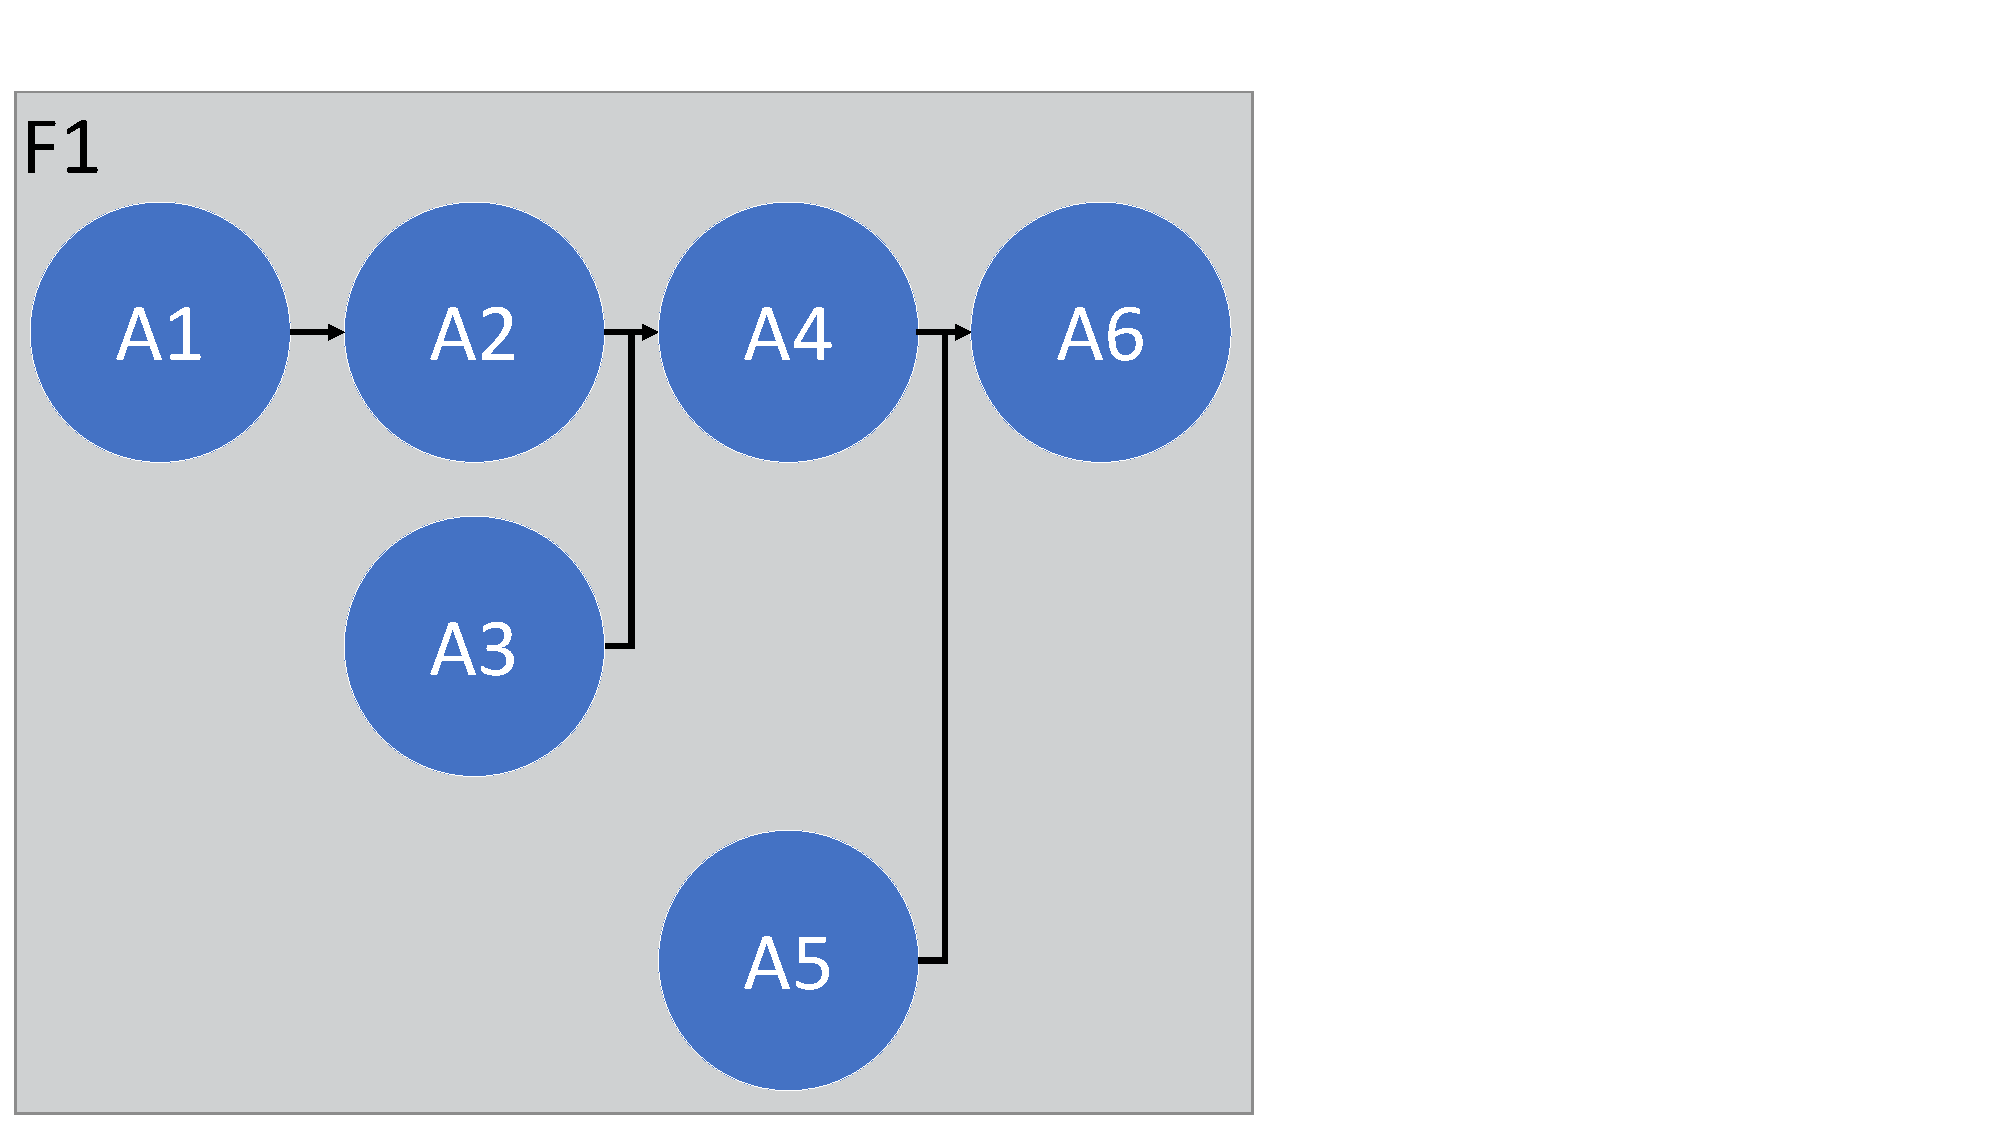
\includegraphics[trim={0cm 0.2cm 12cm 1.6cm}, clip, width=0.35\textwidth]{figures/Artefacts_linking.pdf}
    \caption{Linking of artefacts in the proposed process}
    \label{fig:artefacts_linking}
\end{figure}
%\todo[color=green]{Platz sparen möglich: in der Grafik A5 auf eine Ebene mit A3 bringen}


\begin{figure}[ht]
    \centering
    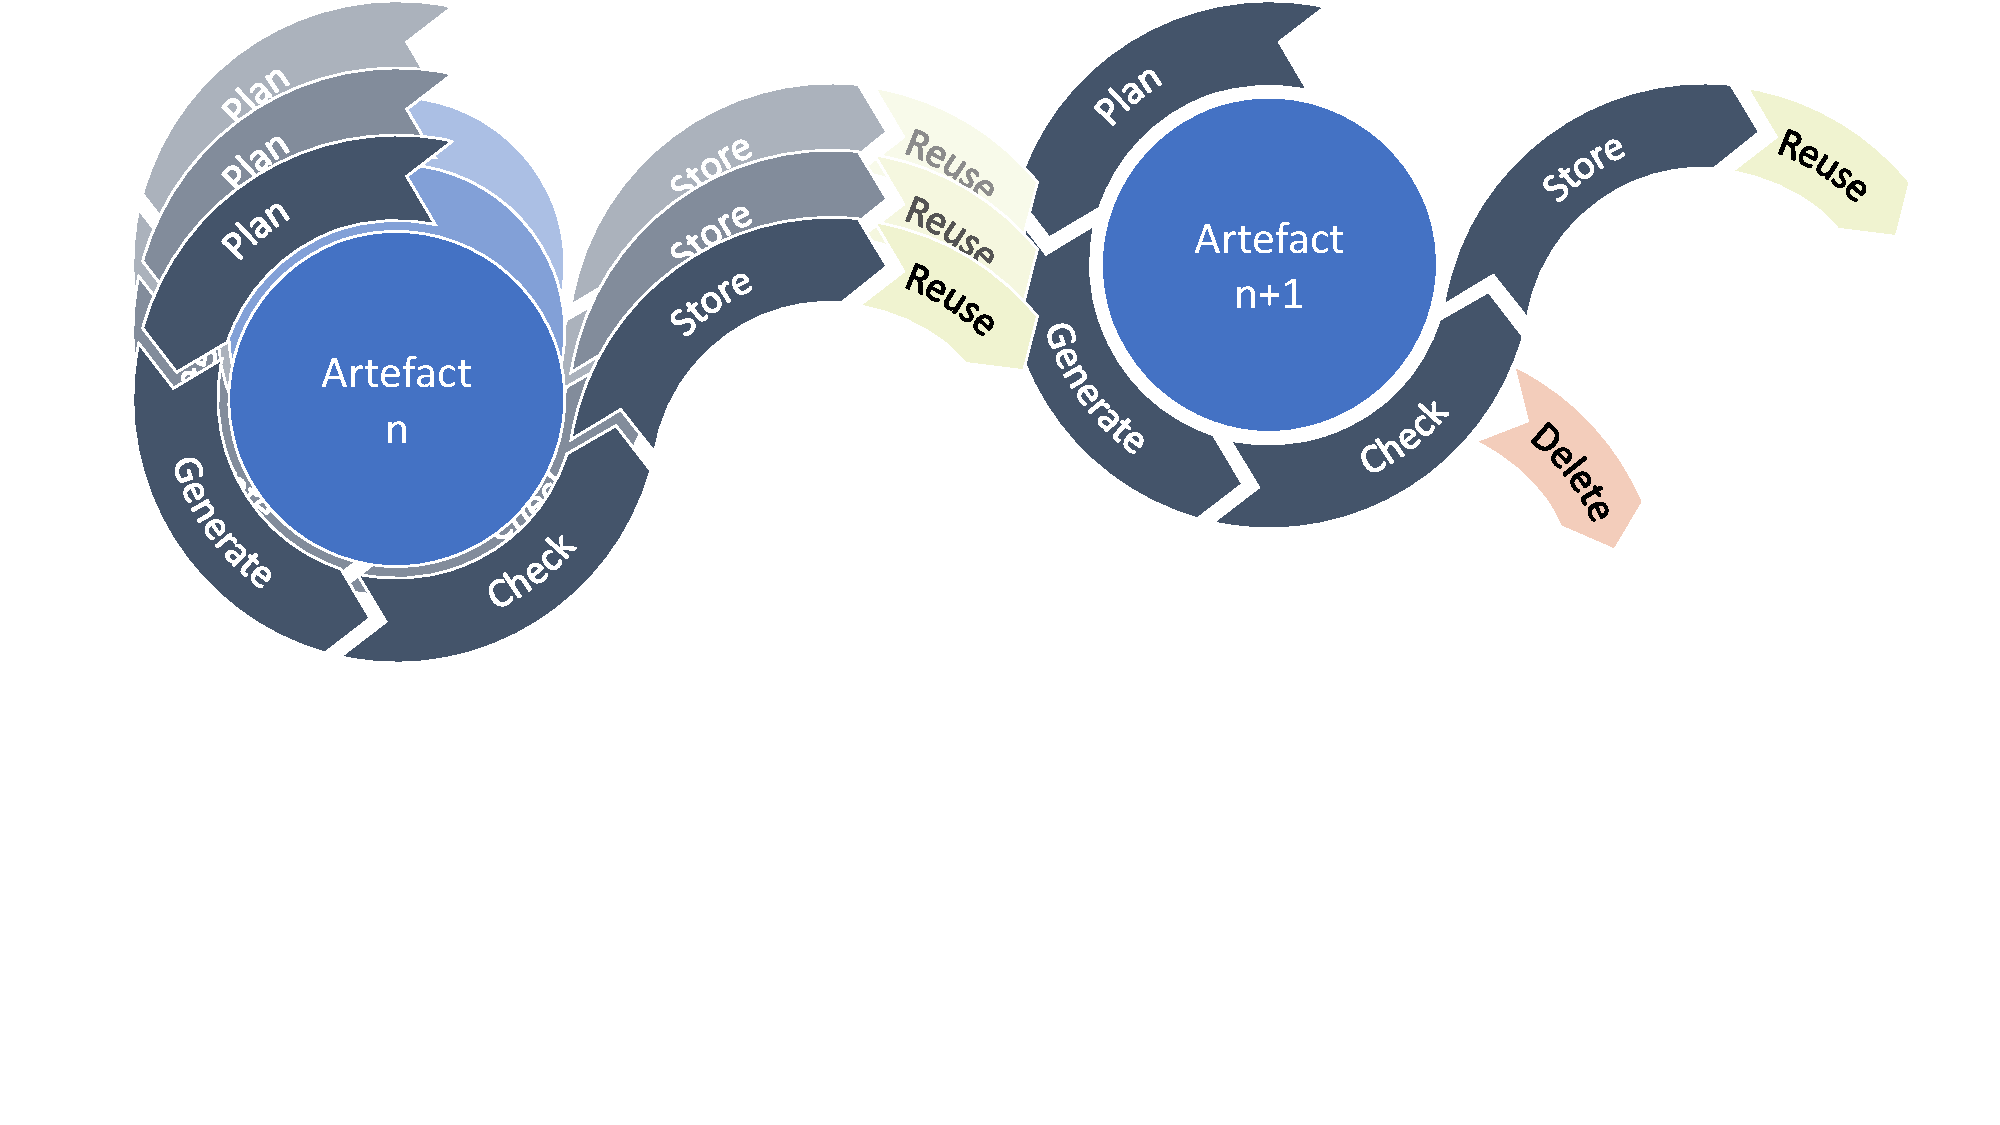
\includegraphics[trim={0cm 7.5cm 0cm 0cm}, clip, width=\textwidth]{figures/Artefact_n21_v2.pdf}
    \caption{Procedure of \ref{Glossary:artefact} linking: Many to one relation}
    \label{fig:Artefact_n21}
\end{figure}


\begin{comment}
\begin{figure}[htbp]
  \centering
  \begin{subfigure}[b]{0.26\textwidth}
    \centering
    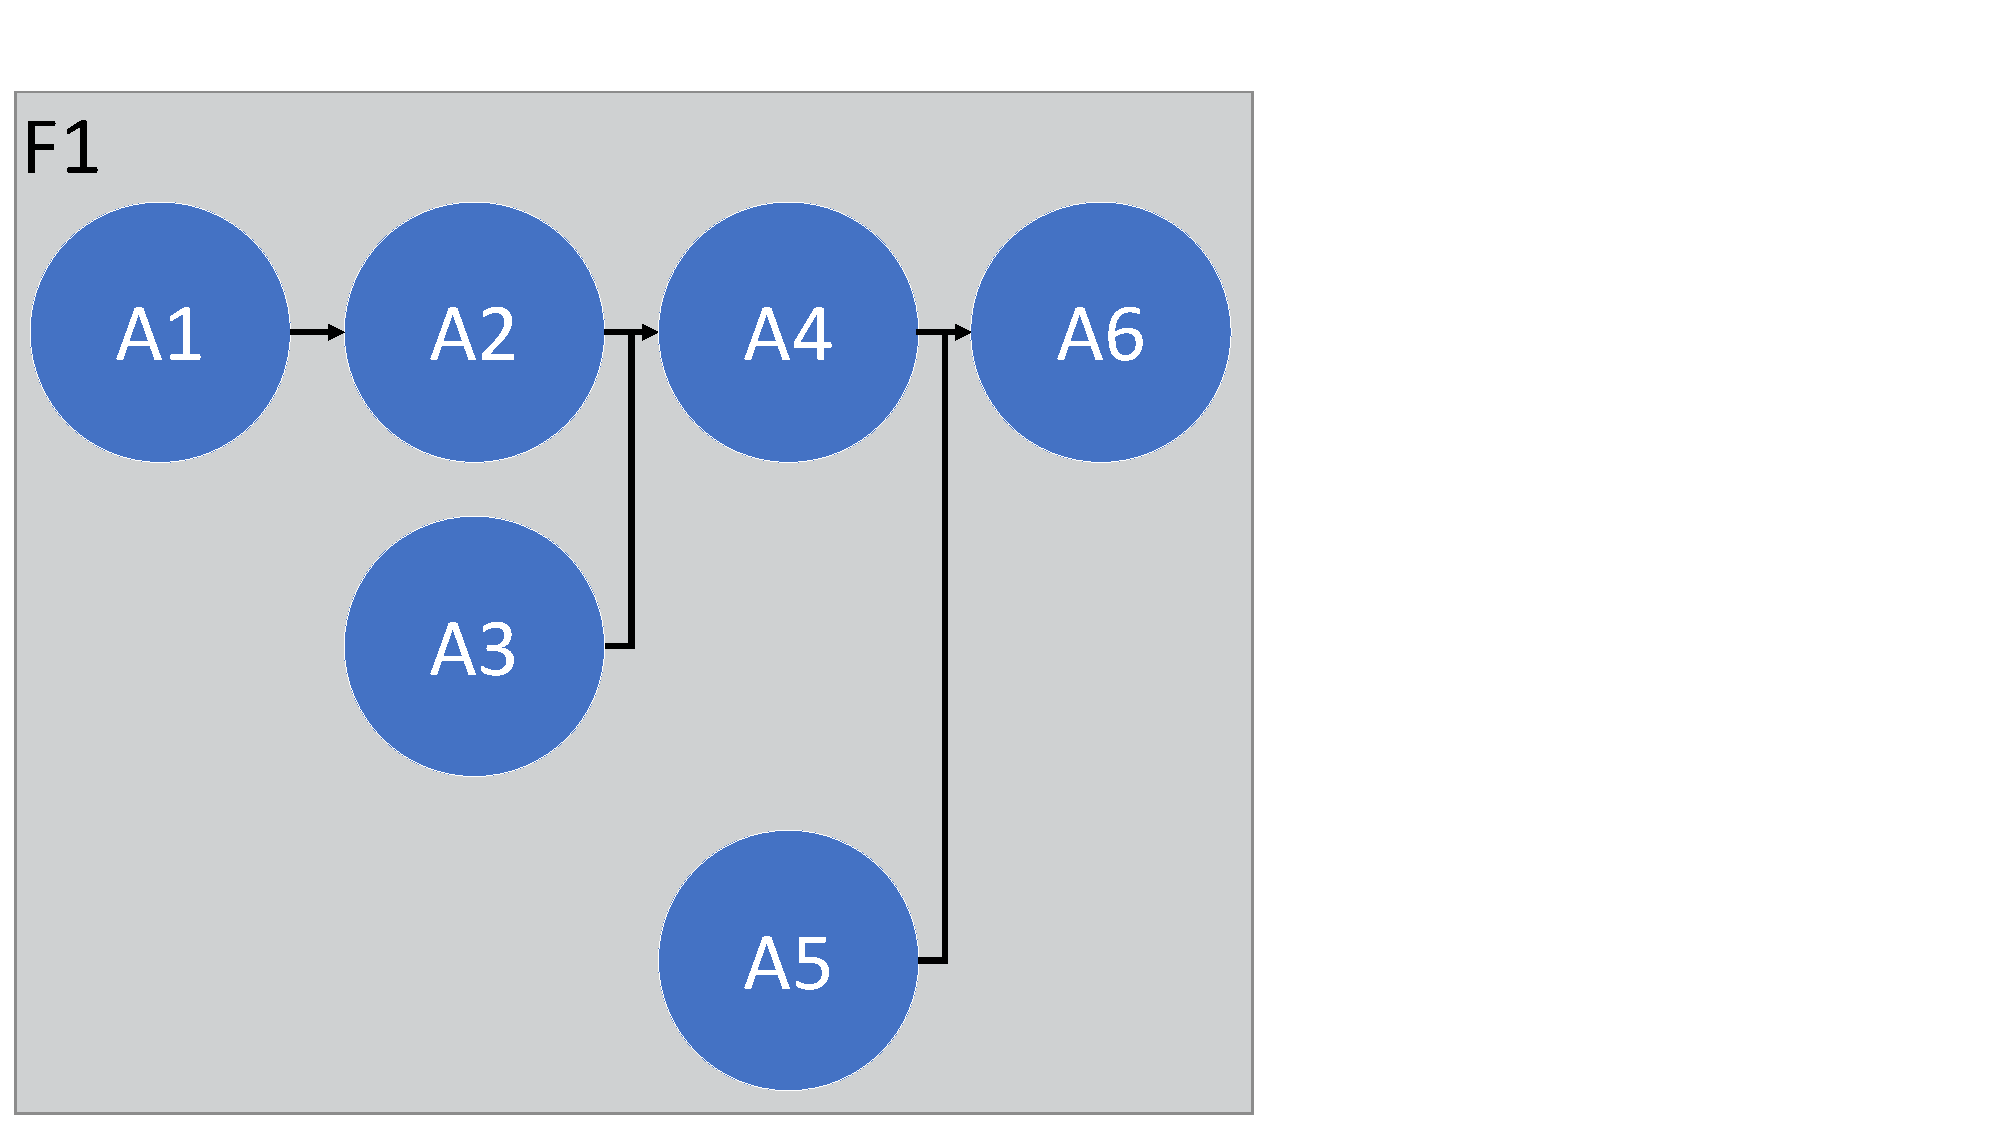
\includegraphics[trim={0cm 0.2cm 12cm 1.6cm}, clip, width=\textwidth]{figures/Artefacts_linking.pdf}
    \caption{Linking of artefacts in the proposed process}
    \label{fig:artefacts_linking}
  \end{subfigure}
  \hfill
  \begin{subfigure}[b]{0.7\textwidth}
    \centering
    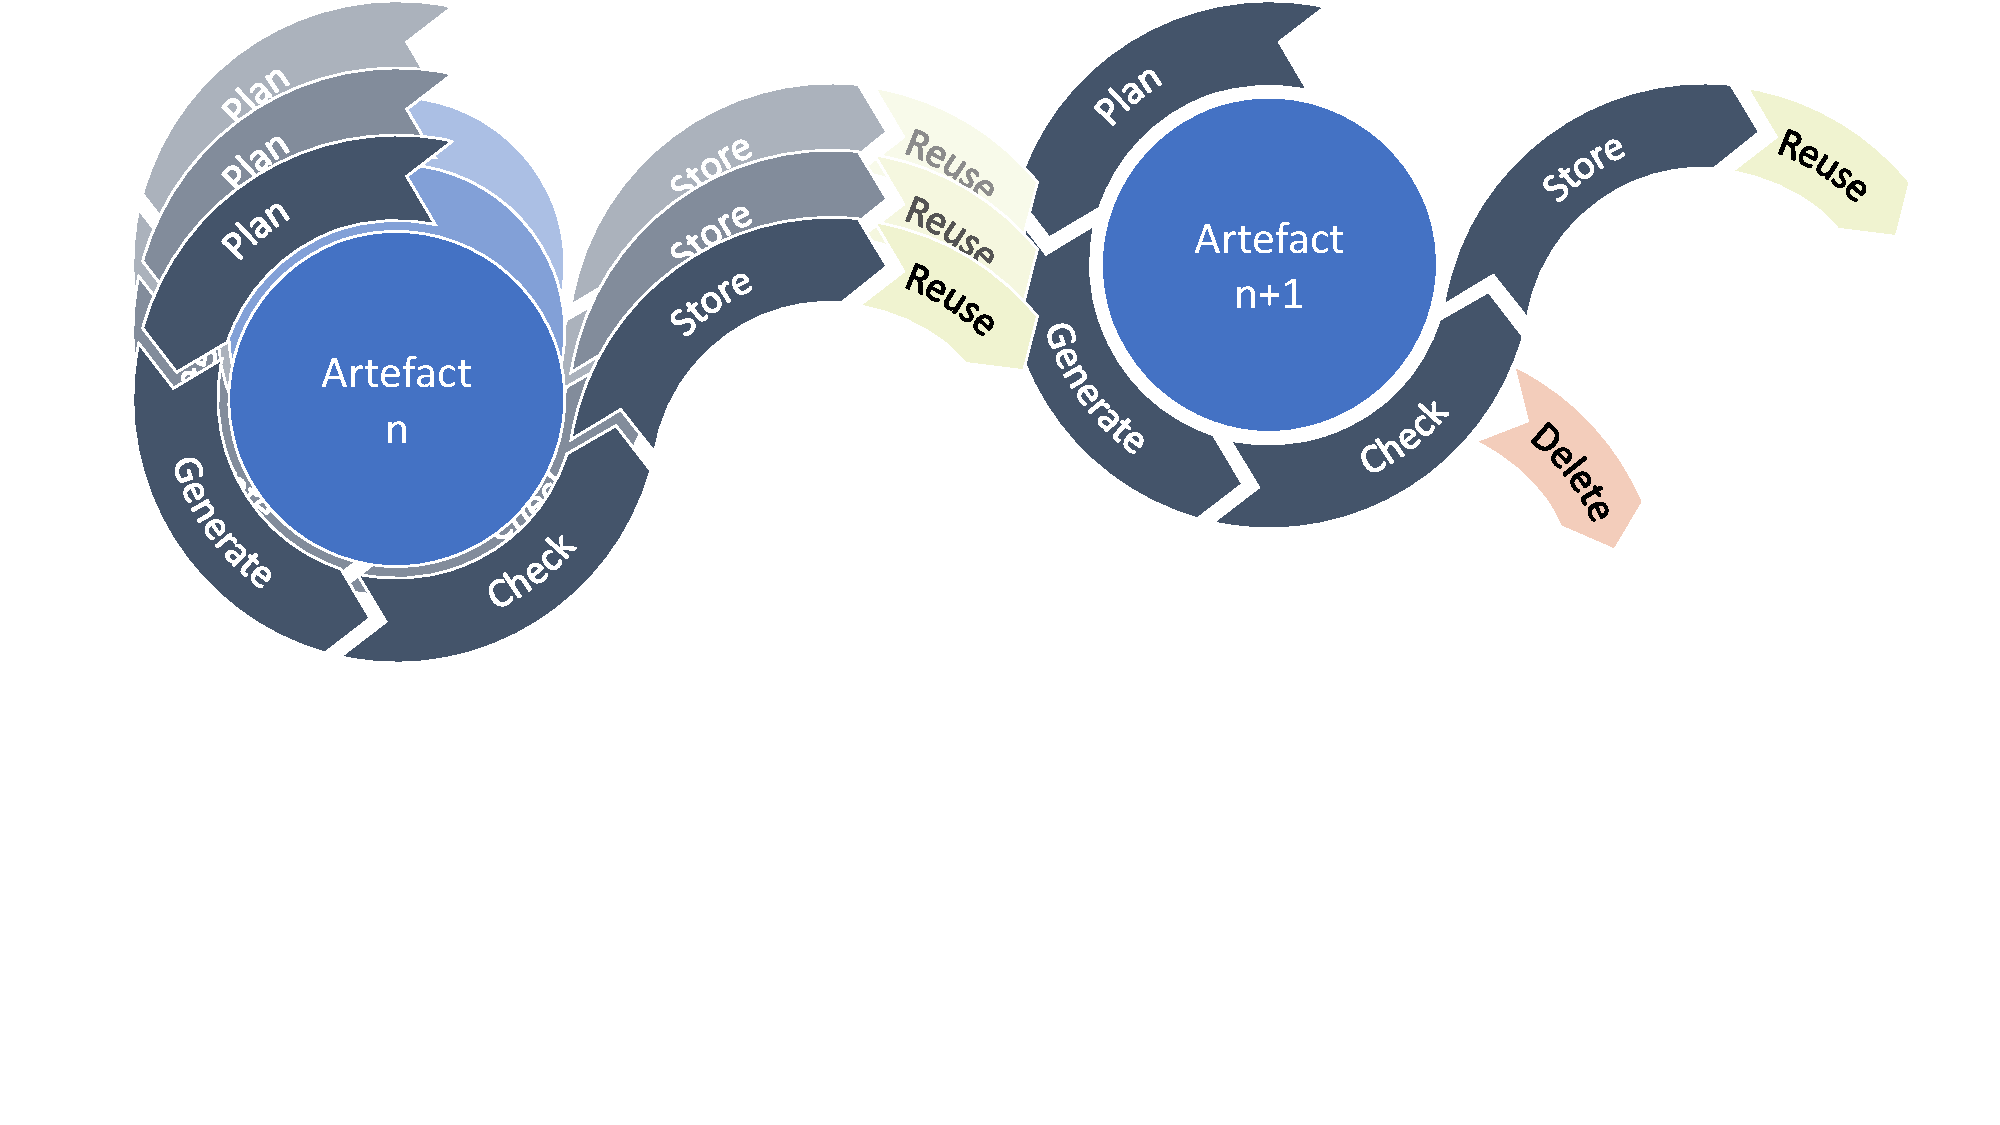
\includegraphics[trim={0cm 7.5cm 0cm 0cm}, clip, width=\textwidth]{figures/Artefact_n21_v2.pdf}
    \caption{Procedure of \ref{Glossary:artefact} linking: Many to one relation}
    \label{fig:Artefact_n21}
  \end{subfigure}
  
  \caption{Contrasting a simple with a more complex \ac{dlc}}
  \label{fig:data_life_cycle_comparison}
\end{figure}
\end{comment}

%Every single time an artefact is created, the \ref{Glossary:generation setup} takes place immediately before the artefact is \ref{Glossary:generate}d.
%While it is \ref{Glossary:generate}d, metadata should be recorded.
%Afterwards it is \ref{Glossary:check}ed  for corruption to \ref{Glossary:ensure} data
%correctness.
%If correct, the artefact is \ref{Glossary:store}d, ideally accessible to project members.
%Hence, an \ref{Glossary:artefact} is planned, contextualised and validated \ref{Glossary:research data} in its smallest unit.


An \ref{Glossary:artefact} may be a primary data collection, a physical object or the implementation of source code, or a collection of secondary data, e.g. from a systematic literature review, as it follows the definition of \ref{Glossary:research data} by the \ac{dfg}:

\hfill\begin{minipage}{\dimexpr\textwidth-0.5cm}
    \textit{
        \enquote{
            Research data includes measurement data, laboratory values, audiovisual information, texts, survey or observation data, methodological test procedures and questionnaires.
            Compilations, software and simulations can equally represent a central result of scientific research and are therefore also included under the term research data. 
            Research data in some subject areas is based on the analysis of objects (such as tissue, material, rock, water and soil samples, test specimens, installations, artefacts and art objects), so its handling must be just as careful and consideration must be given to a technically adequate option for subsequent reuse whenever meaningful and possible. 
            Should subsequent reuse of the resulting research data be closely associated with objects, then please also elaborate on this by providing all relevant information. 
        } \cite{GermanResearchFoundation.2015}
    }
\end{minipage}
%\todo[color=green]{Bei Bedarf Platz sparen: wörtliches Zitat löschen oder paraphrasieren}


%\todo{MR: Kannst du das noch in citavi korrekt aufnehmen? https://www.dfg.de/resource/blob/174736/forschungsdaten-checkliste-en.pdf Bin unsicher, welcher typ das ist.}

To elaborate further: As defined by North \cite{North.2021} with the model of the knowledge stairway, data is a number of characters (numbers, letters, special characters) that are related to each other by syntax (ordering rules). 
The metadata recorded along with the generation of the data adds context - i.e. a meaning - to it, so data becomes an \ref{Glossary:artefact}, which is on the information step at the knowledge stairway. %\todo{MR: Wissenstreppe}

If the artefact is a physical object, the data is contained within the object, ready to be analysed and further processed in an analogue or digital way. \cite{Rixen.2026, Plomp.2021, Schilthuizen.2015}
The biggest differences in physical data is their storage and indivisibility.
An object can not be made publicly available and is stored in a physical rather than a digital storage.
Yet, it has a (physical) address and access requirements that shall be clarified just like with a digital object.


%\todo[inline]{Wording/Explanation: Hardware muss als artefakt betrachtet werden}
%\todo[inline]{5. Beispiel aufnehmen, wie das in zwei Artefakte aufgeteilt ist, Stichwort Labeling - 6. s. anderen Konflikt mit den Labels}
%\todo[inline]{Granularität Artefakte, digital object?}
%\todo[inline]{2.8.  R: Ähm, kann natürlich teilweise sein, dass Artefakte, mit denen man je nachdem wie man die Artefakte definiert, kann es natürlich auch sein, dass man mit Artefakten schon weiterarbeitet, obwohl sie gar nicht noch nicht gecheckt sind. Wenn Sachen zum Beispiel parallel entwickelt werden, ist halt die Frage, wie definiert man das Artefakt und wie kleinteilig macht man das? (..)"}
%\todo{das muss ich noch im glossar umbauen--> TH}
%\todo{Digital Objects referenzieren --> TH}

No changes were made to the definition of \ref{Glossary:finding}s.
However, and according to North's knowledge stairway \cite{North.2021}, the \ref{Glossary:finding compilation} was more explicitly focussed on the generation of knowledge: If several pieces of information (\ref{Glossary:artefact}s) are networked and related to each other, knowledge is created. So a \ref{Glossary:finding} is knowledge, as, according to North \cite{North.2021}, knowledge is a semantically interconnected information.
As a finding is compiled by the interconnection of artefacts, which are bits of information, it is knowledge.

%\todo[inline]{Als Beispiel für Finding (Artefakt + Artefakt Validierung = Finding) im Paper aufnehmen}

%\todo{Ensure als wording festlegen}
%\todo[inline]{Ensure: Spätestens hier muss das passieren}
%\textcolor{red}{}

\subsection{Feedback on the project management level}
\label{TopFeedback}

One of the most controversially discussed parts of the proposed process is the \ref{Glossary:project management level}, now adjustified to \ref{Glossary:project level}. 
Figure \ref{fig:DescriptiveFeedback_top} shows the codes found for this level in general as well regarding certain parts of it.

\begin{figure}[ht]
    \centering
    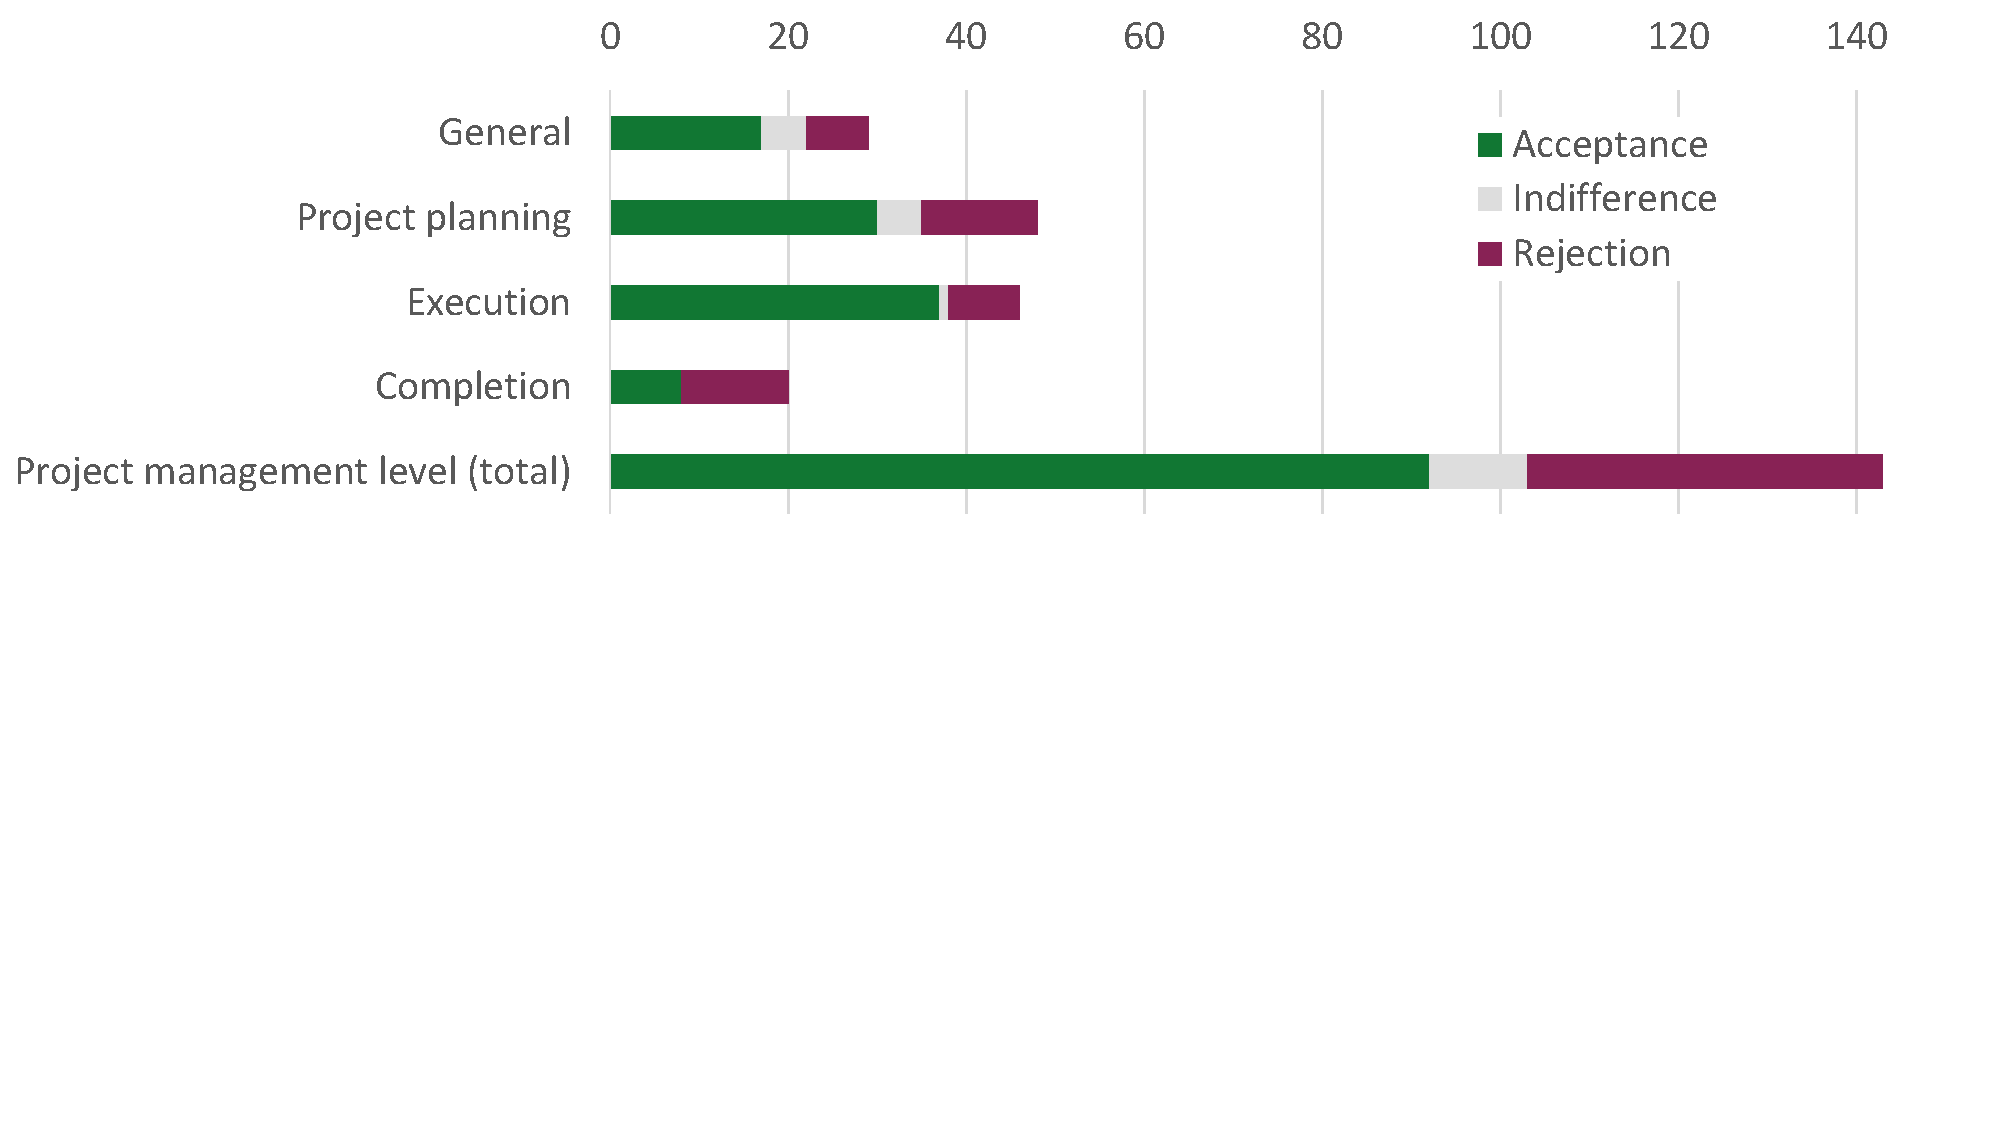
\includegraphics[trim={0cm 10.25cm 0cm 0cm}, clip, width=\textwidth]{figures/Table3_Figure.pdf}
    \caption{Codes on the feedback received on the project management level. The exact numbers can be found in table \ref{tab:DescriptiveFeedback_top} in the appendix.}
    \label{fig:DescriptiveFeedback_top}
\end{figure}

%\todo[color=green]{Bei Bedarf Platz sparen: Tabellen auskommentieren oder in den Anhang}

% T - General - Done
%\todo[inline]{Manchmal doch iterativ}
%\todo[inline]{Top level kein Waterfall, ist auch iterativ}
%\todo[inline]{Im Paper: Diskussion Wasserfall toplevel}
Most of the attention points on the \ref{Glossary:project level} focussed on its waterfall-like design.
Some interviewees claimed, that it would still be iterative.
These comments especially refer to the demarcation between \ref{Glossary:execution} and \ref{Glossary:completion}.
Furthermore, some interviewees annotated, that this distinction is not as clear as between \ref{Glossary:project planning} and \ref{Glossary:execution}, while others emphasised it particularly as clear-cut.
%\todo[inline]{Zeit zwischen T1 und T2 z.T. lang}
% \todo[inline]{Pause zwischen den Phasen haben wir noch nicht berücksichtigt}
The acceptance of a \hyperref[Glossary:research proposal]{research proposal} marks the transition. 
A \hyperref[Glossary:research proposal]{research proposal} may be not just a funding proposal but any proposal made to anyone to conduct a research \ref{Glossary:project}, e.g. to industry partners.
It could also be seen as, for example, a proposal for a dissertation made to a professor. The acceptance of a \hyperref[Glossary:research proposal]{research proposal} or the determination of the projects completion phase can be seen as a kind of quality gate, similarly to the concept of quality gates promoted in Prefi \cite{Prefi.2014} or Hawlitzky \cite{Hawlitzky.2002}: When a quality gate is reached in the process (e.g. the transition from \ref{Glossary:project planning} to \ref{Glossary:execution}), a \ref{Glossary:check} is performed to determine whether the activities carried out so far are sufficient (e.g. acceptance of the \hyperref[Glossary:research proposal]{research proposal}). If not, the quality gate cannot be passed, meaning activities must be repeated before the next phase can begin. %\todo[color=red]{@TH: Welches Kapitel hast du hieraus zitiert? --> Ich würd nochmal gern das Werk ändern. Es ist dann https://doi.org/10.1007/978-3-446-43992-4            und da Kapitel 19.6 - Quality Gates steuern die Qualität im Produktentstehungsprozess, Seiten 412-427 }
%\todo{Quelle Quality Gates HAWL02, PFEI07}

Every part of work performed before the acceptance is seen as \ref{Glossary:preparatory work}: may be an early start, if the \ref{Glossary:project} is very likely going to be accepted,  may be \enquote{quick and dirty} data, not worth of publishing, yet able to give away \ref{Glossary:finding}s.
\hyperref[Glossary:preparatory work]{Preparatory work} follows the principles of \ref{Glossary:content-wise execution} in its approach.
Consequently, the data \ref{Glossary:generate}d in \ref{Glossary:preparatory work} can be handled the same way as data created in the \ref{Glossary:execution}.
Furthermore, data used in \ref{Glossary:preparatory work} can also be a result of a predecessor \ref{Glossary:project}, which means, \ref{Glossary:artefact}s are reused for the new \ref{Glossary:project}'s planning.


For the transition between \ref{Glossary:execution} and \ref{Glossary:project completion}, the interviewees agreed that research is a never ending process; its completion is only achieved when the relevant demands are satisfied.
There will always be something to look deeper into or reconsider or research more on.
Hence, the transition to the \ref{Glossary:project completion} phase takes place once the supervisors for the \ref{Glossary:ongoing project management} determine that one or more of the following conditions are met:

\begin{itemize}[noitemsep]
    \item The \ref{Glossary:finding}s \ref{Glossary:generate}d in the \ref{Glossary:project} suffice to answer the overarching research question
    \item The \ref{Glossary:project}'s time frame has ended
    \item The \ref{Glossary:project} funding has run out
\end{itemize}

In the \ref{Glossary:project completion}, the ensuring of reproducibility is an important task as it has to be seen as re-considering the work done and validating that it was done correctly: The term \ref{Glossary:ensure} was specified and means, that a verification and affirmation, if an activity has been performed, is conducted. 
If the activity was not conducted at the point of ensuring it, it has to be performed latest at this point when the ensuring takes place. 
Ideally, the \ref{Glossary:ensure}d activity was performed beforehand.



%\todo[inline]{Quality gates auf top level! ggf auch auf mid und low?}
%\todo[inline]{Quality gates}
%\todo[inline]{Quality Gate wegen Pause, Antrag überarbeiten Projekt abbrechen im Text erwähnen? Projekt nicht erfolgreich?}
%\todo[inline]{Completion und Execution are not always this strictly divided}

\iffalse
% Zwischenschritt, kann nachher auskommentiert werden
\begin{figure}[ht]
    \centering
    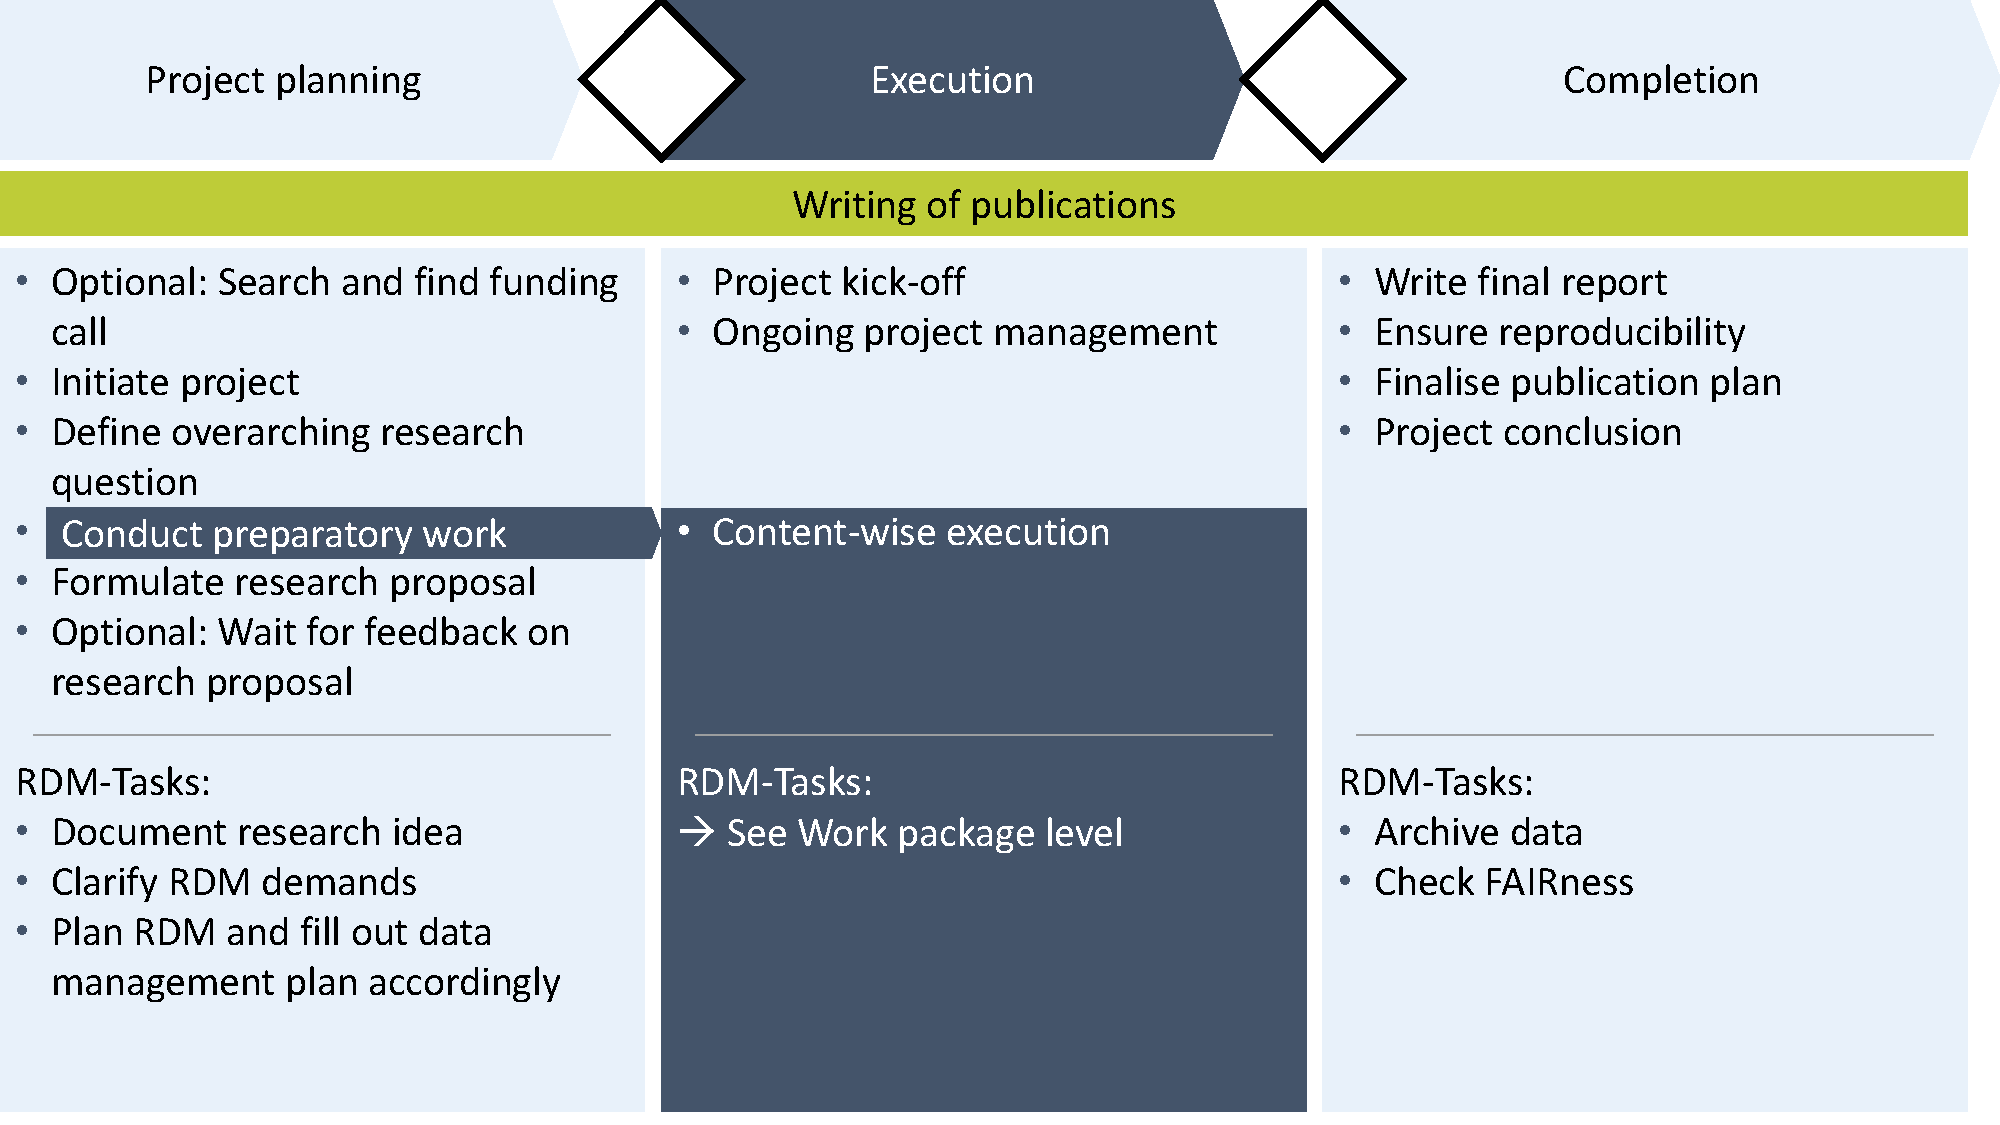
\includegraphics[trim={0 1.5cm 0cm 0cm}, clip, width=\textwidth]{figures/Top_level_v2.pdf}
    \caption{The redesigned project level of the proposed research process}
    \label{fig:Top_level_v2}
\end{figure}
\fi

% T1 - Done
%\todo[inline]{Preperatory work: 1. Eigenes mini projekt, 2. außerhalb von projektstrukturen?, 3. Steht einfach in T1 mit drin --> Was passiert, wenn da jetzt forschungsergebnisse generiet werden?}
%\todo[inline]{Preparatory work kann aus aktuellem Projekt kommen (ist dann Nachfolgeantrag oder Diss)}
%\todo[inline]{Preparatory work besser defnieren - ist ein Reveiw Paper zur Vorbereitung schon ein Finding? Oder Vorlaufforschung?}
%\todo[inline]{Daten in execution phase sind gut, Daten in preparatory work sind quick and dirty}
% \todo[inline]{Conduct/Collect preperatory work}
%\todo[inline]{Search/Find funding call optional}
%\todo[inline]{DMP anfertigen}
%\todo[inline]{Prozess ist bei industrieprojekten anders, keine antragssuche --> research proposal kann antrag sein, kann diss sein, kann industrieangebot sein}
%\todo[inline]{Parallel kann projekt oder parallelprojekt schon bearbeitet werden, wenn wahrscheinlichkeit hoch, dass förderung kommt}
%\todo[inline]{Kann nach antrag einreichung sehr großten zeitraum haben}


% T2 - Done 
%\todo[inline]{Team in Excecution kann ganz anderes als beim antrag sein --> überleitung zu T1 lücke}
%\todo[inline]{Project kick-off and Initialisierung Projektmanagement}
%\todo[inline]{Daten in execution phase sind gut, Daten in preparatory work sind quick and dirty}
%\todo[inline]{Im ongoing project management müssen Anpassungen in der Planung explizit, nicht nur implizit aufgenommen werden.}
%\todo[inline]{DMP updaten}
%\todo[inline]{Ongoing project management können auch Zwischenberichte sein + Punkt mit dem Folgeantrag}
%\todo[inline]{41. Abgleich, ongoing project management}
%\todo[inline]{Zwischenberichte}
%\todo[inline]{In Execution können dinge anders laufen als in der planung}
%\todo[inline]{Project-Kick Off: Man muss erstmal wieder ins projekt reinkommen}
% \todo[inline]{In T1 und T2 werden daten erzeugt, in T1 sind die daten aber quick and dirty}



In the \ref{Glossary:execution} phase only few attention points were brought up by the interviewees.
Most importantly, the \ref{Glossary:ongoing project management} has to be specified.
It holds not only typical tasks like comparing the \ref{Glossary:project} plan to the current status but also encompasses the writing of intermediate reports and considerations regarding follow up \ref{Glossary:project}s.
It also has to be considered that unforeseen challenges arise, demanding adaption of the original plans. 
The \ref{Glossary:ongoing project management} defines the next \ref{Glossary:finding} that should be \ref{Glossary:generate}d based on the work done with previous \ref{Glossary:finding}s, which are adapted, if needed.
%\todo{das hier ist super wichtig!}
This decision is done at the \ref{Glossary:project} management when a \ref{Glossary:finding} is compiled.

\iffalse
% Zwischenschritt, kann nachher auskommentiert werden
\begin{figure}[ht]
    \centering
    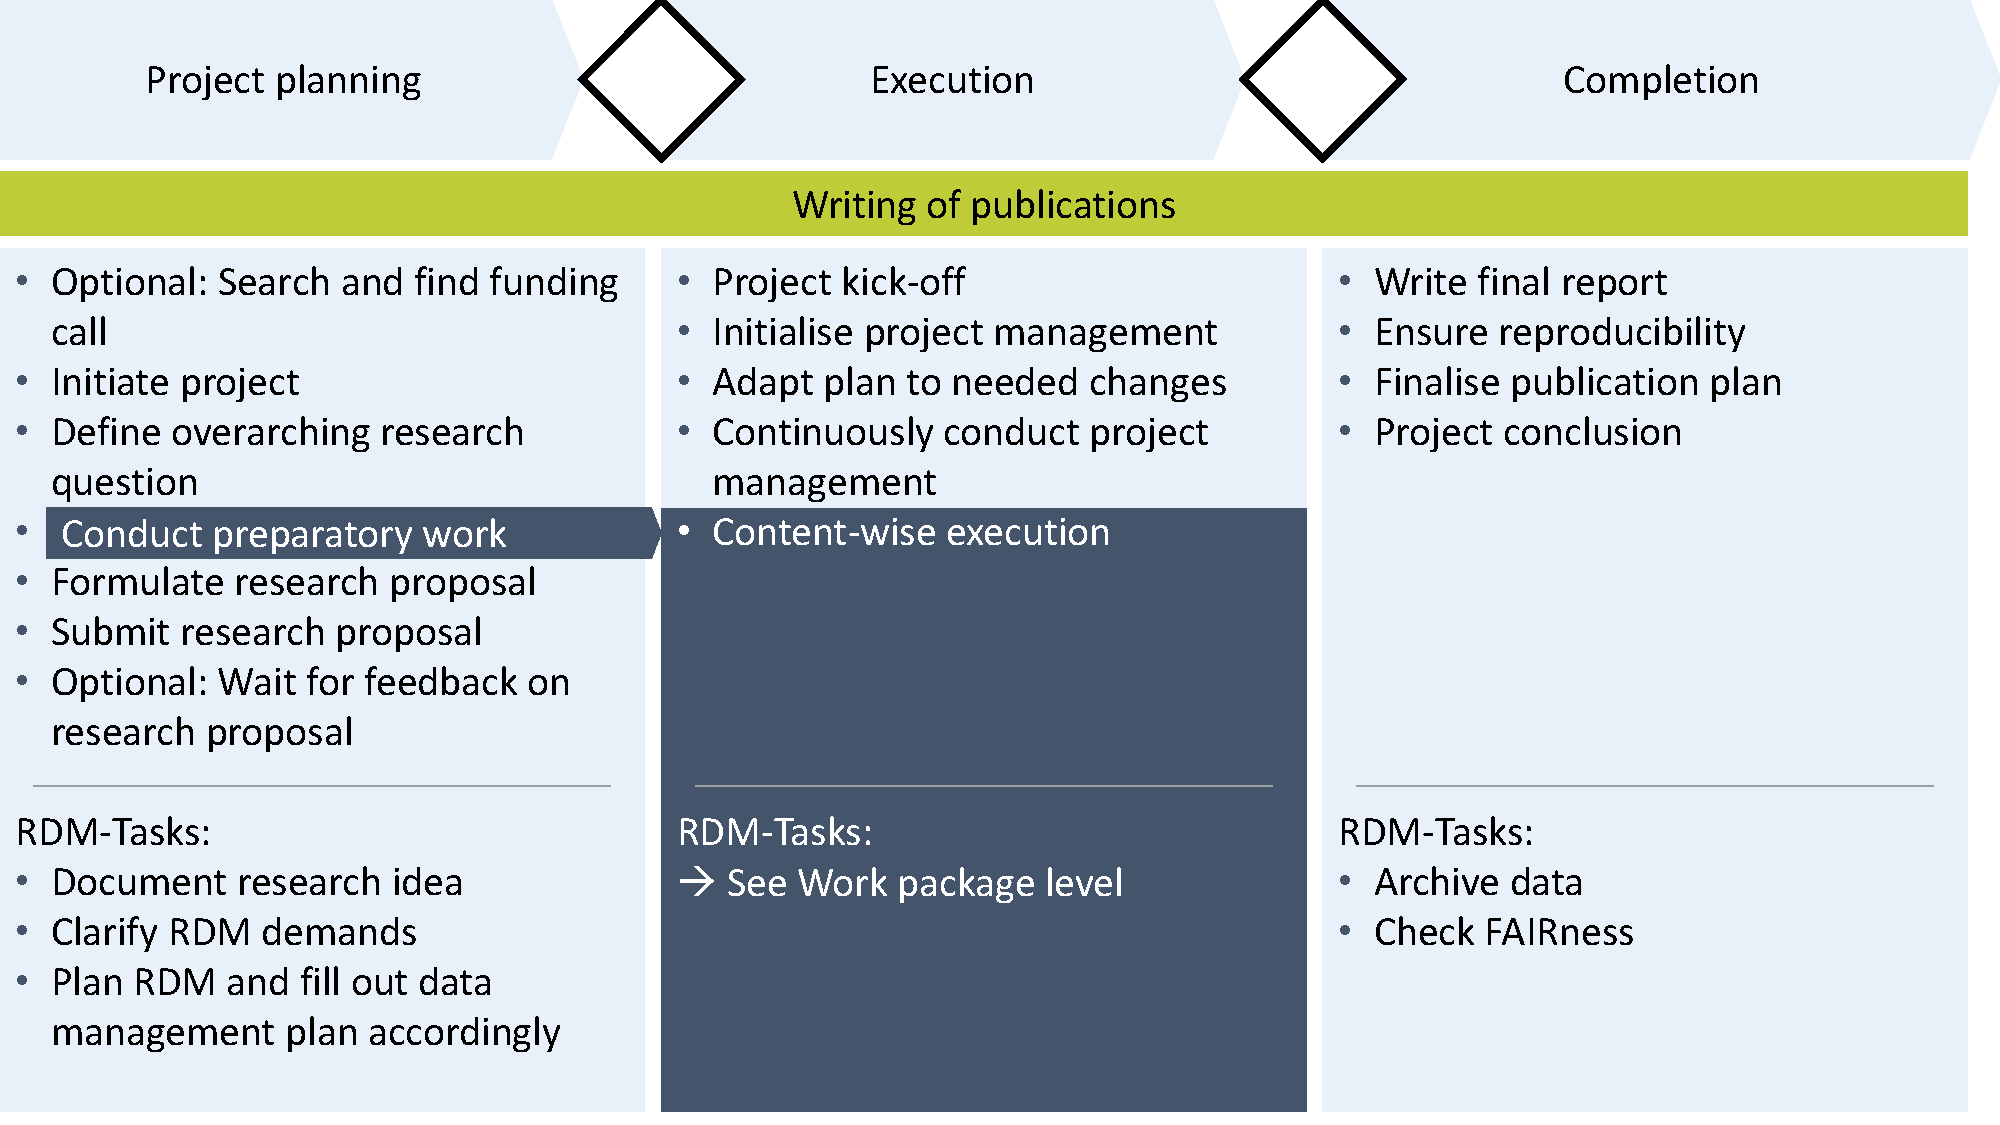
\includegraphics[trim={0 0.5cm 0cm 0cm}, clip, width=\textwidth]{figures/Top_level_v3.pdf}
    \caption{The redesigned project level of the proposed research process}
    \label{fig:Top_level_v3}
\end{figure}
\fi

% T3 - Done
%\todo[inline]{Reproduzierbarkeit sicherstellen, sofern möglich}
%\todo[inline]{Reproduzierbarkeit kann nicht immer sichergestellt werden, und ist oft auch nicht von interesse}
%\todo[inline]{Reproduktion der Ergebnisse wird in Praxis nicht immer berücksichtigt}

%\todo[inline]{8: Abschlussbericht: Unterschiedliche Interpretationen möglich}
%\todo[inline]{Folgeantrag}
%\todo[inline]{Nachfolgeantrag schreiben}
%\todo[inline]{Berücksichtigung von Folgeaktivitäten (Folgeprojekt, Diss, Produktivbetrieb etc.) in Übersichtsgrafik als Pfeil wie Publikationsprozess --> Könnte das nicht jederzeit passieren?}

%\todo[inline]{\enquote{Was man bis dahin nicht gemacht hat, wird man auch später nicht mehr retten können}}

%\todo[inline]{Wording: Publikationen fertigstellen, nicht Plan}
% \todo[inline]{Completion ist project completion}
%\todo[inline]{Wording: Projekt Completion}
%\todo[inline]{gibt mehrere quasi Completions haben wir de facto auch getrennt. Also die Completion, die hier steht, ist wirklich die Projekt Completion. Müssen wir vielleicht im Naming auch noch mal anpassen}
%\todo[inline]{Frage. Wann ist Projekt Completion? Kein geld mehr? Work Packages done?}
%\todo[inline]{Forschungsfragen sind nie vollständig beantwortet, sondern man kann immer noch tiefer gehen, noch mehr forschen. Projekt ist abgeschlossen, wenn die projektziele erreicht wurden}

Based on the interviewees, ensuring reproducibility can be challenging to impossible some times.
Some experiments are unique and will never be able to be reproduced, e.g. the recording of a supernova\footnote{Example changed due to anonymisation.}.
Hence, the exact wording of this point has been changed.
It also has to be annotated that some interviewees do not see the ensuring of reproducibility as important. This can be condensed to one statement in particular: \enquote{\textit{What you haven't done by then, you won't be able to save later on either.}}
Still, ensuring of reproducibility is an important task, yet coming back to the aforementioned wording of \textit{\ref{Glossary:ensure}} as re-considering the work done and validating that it was done correctly.

Furthermore, the interviewees annotated that the \ref{Glossary:project completion} phase often already considers follow-up \ref{Glossary:project}s.
For instance, if the prolongation of a \ref{Glossary:project} is already considered guaranteed, the \ref{Glossary:project completion} is not seen as strict as without a follow-up \ref{Glossary:project}.

Also, the interviewees pointed out that \ref{Glossary:publication}s could be started at any given stage of the research \ref{Glossary:project}.
Specific triggers for \ref{Glossary:publication}s are discussed in section \ref{PublicationFeedback}.
After its redesign, the new process for the \ref{Glossary:project level} of the proposed research process is shown in figure \ref{fig:Top_level_redesign}.

\begin{figure}[htbp]
    \centering
    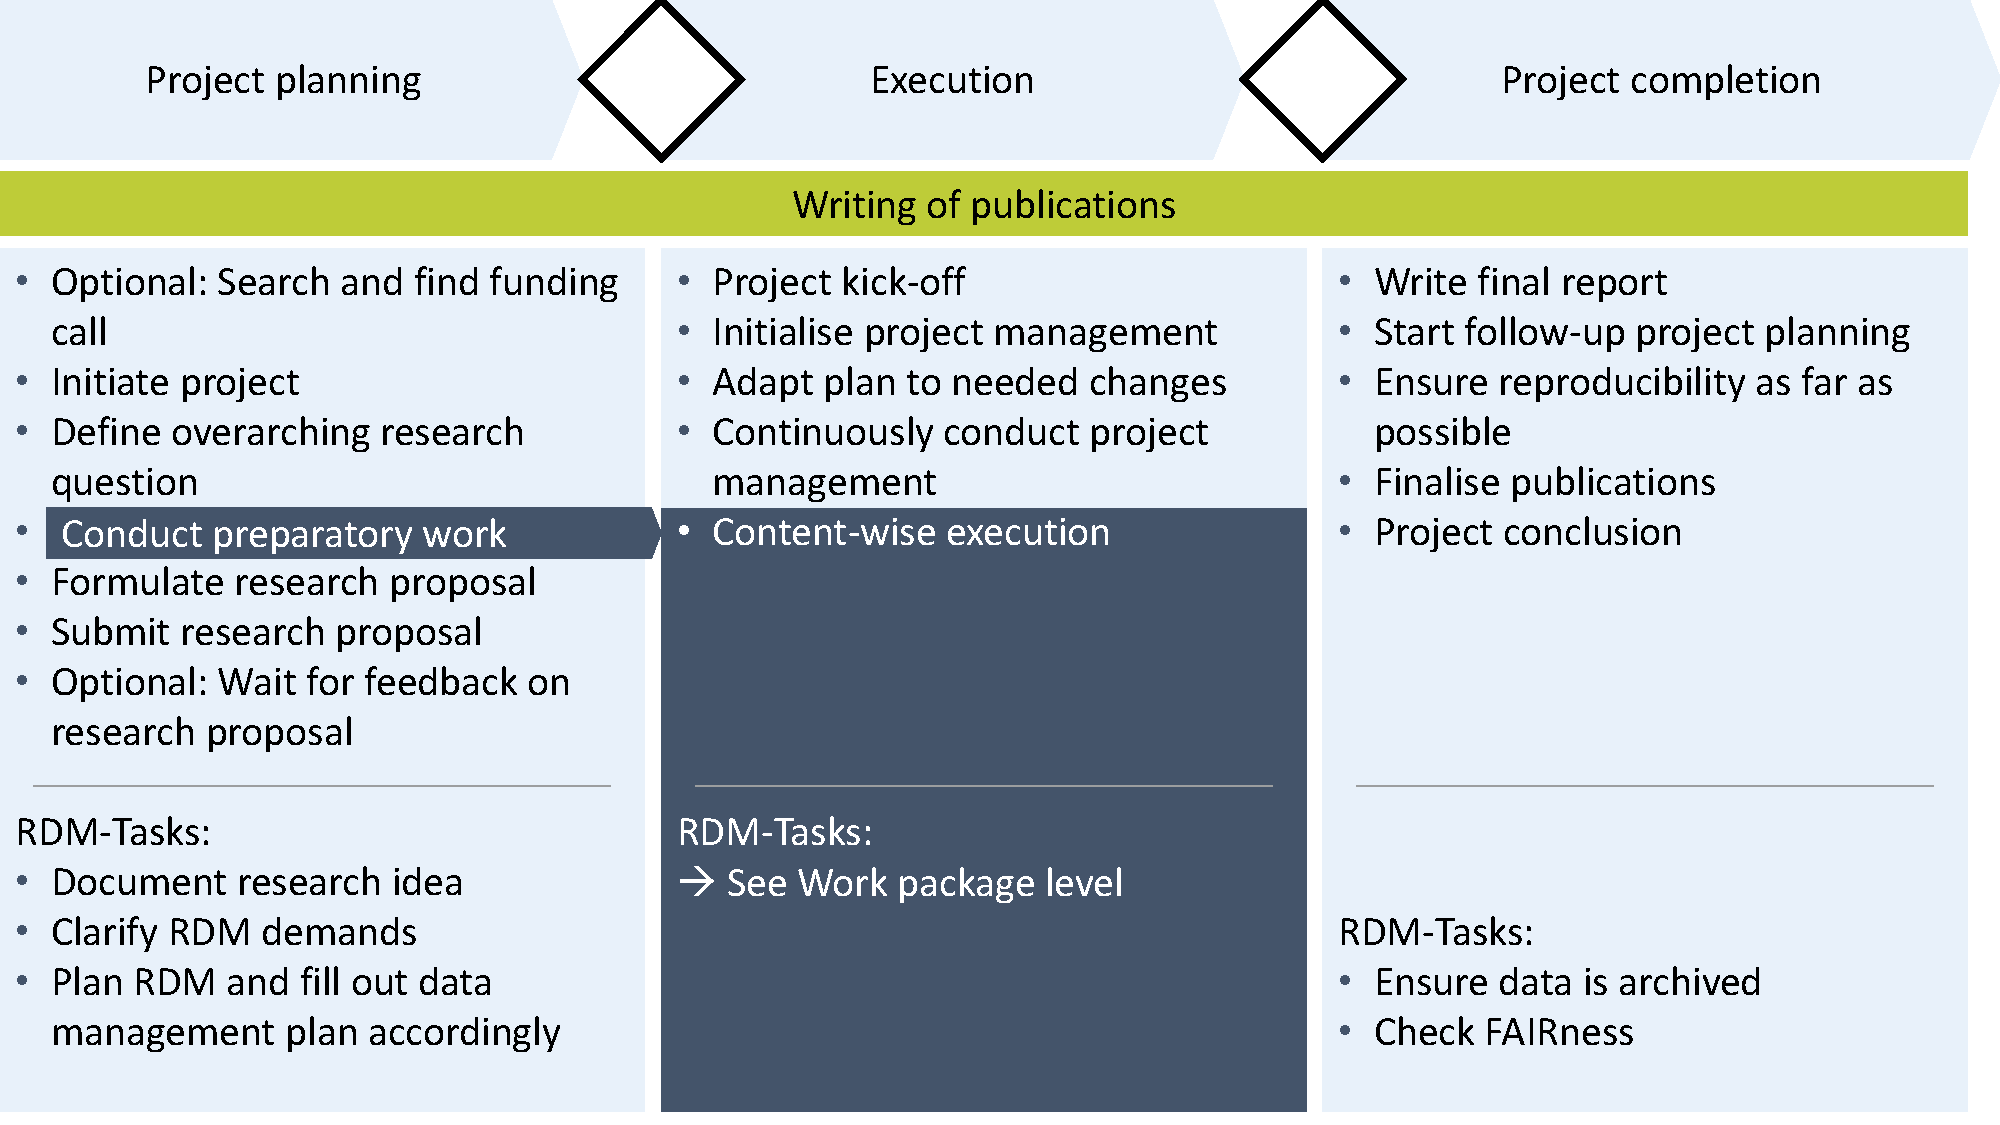
\includegraphics[trim={0 0.5cm 0cm 0cm}, clip, width=\textwidth]{figures/Top_level_v4.pdf}
    \caption{The redesigned project level of the proposed research process}
    \label{fig:Top_level_redesign}
\end{figure}

\subsection{Feedback on the work package management level}
\label{MidFeedback}

The work package management level also offers some opportunities of improvement, both in wording as well as overall process structure.
The discussions with the interviewees focussed on two points in particular.
On the one hand, they empathized the importance of this level being of an iterative nature, as sometimes \ref{Glossary:finding}s will result in discovering new directions worth investigating.
On the other hand, the \ref{Glossary:finding compilation} is seen as debatable in the proposed state.
Figure \ref{fig:DescriptiveFeedback_mid} shows the codes found for the level.

\begin{figure}[ht]
    \centering
    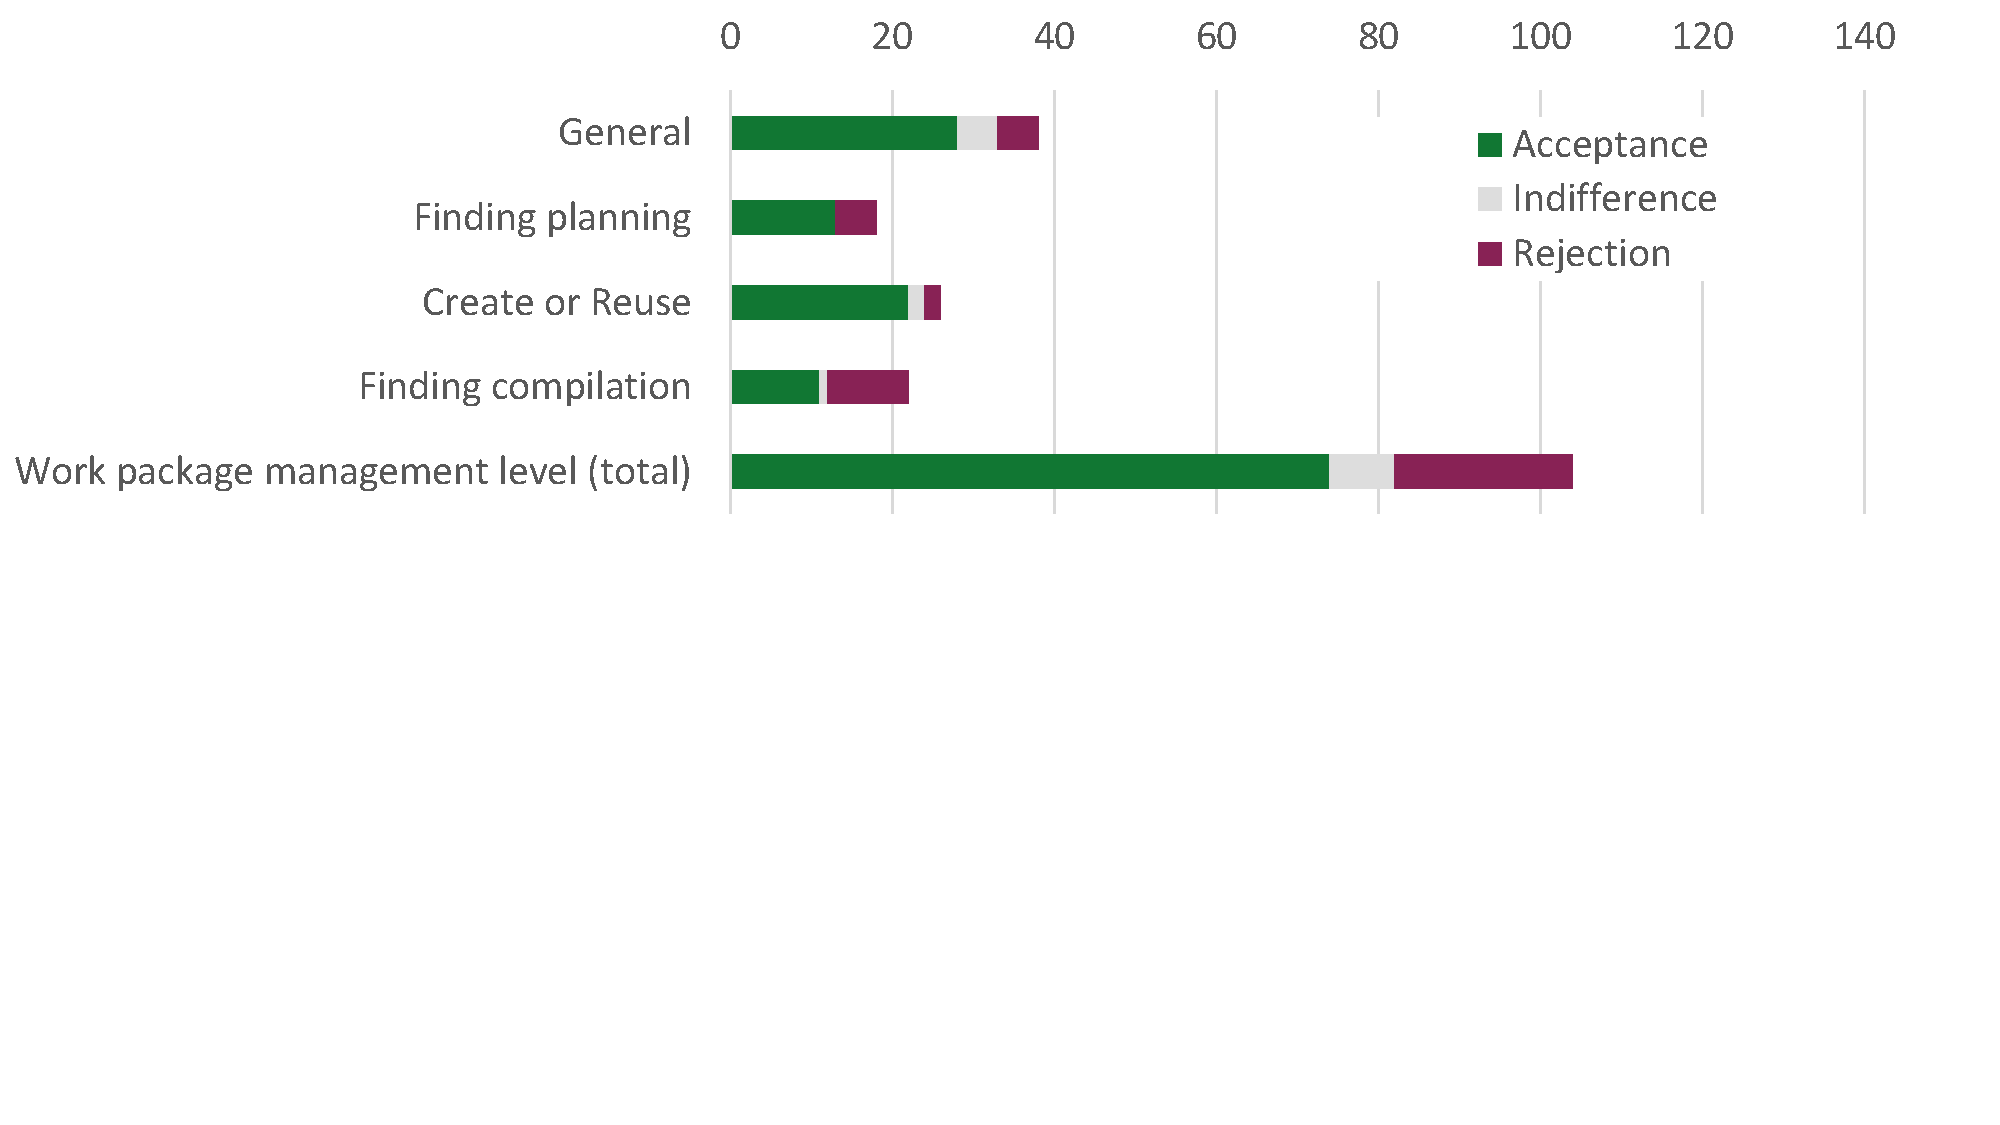
\includegraphics[trim={0cm 10.25cm 0cm 0cm}, clip, width=\textwidth]{figures/Table4_Figure.pdf}
    \caption{Codes on the feedback received on the work package management level. The exact numbers can be found in table \ref{tab:DescriptiveFeedback_mid} in the appendix.}
    \label{fig:DescriptiveFeedback_mid}
\end{figure}

% General - Done
The work package management level is seen under a completely new perspective:
As the interviewees pointed out, the former designation does not properly represent the nature of research.
Rather, the level needs to be separated from the perspective of work packages and has to focus on the \ref{Glossary:finding} aspect of research instead.
This way, uncertainties with wording and the scope of the level are addressed:
The level is now called \ref{Glossary:finding level}.


% Struckture of the mid level
%\todo[inline]{Quality gates auf top level! ggf auch auf mid und low?}
%\todo[inline]{Ist Low Level Iterativ, oder ist nur Mid Level Iterativ?}
%\todo[inline]{Arbeitspakete können parallel sein --> explizieren}
%\todo[inline]{2.5. das sind Findings, mit denen hat man nicht gerechnet. Ich glaube, deswegen ist es auch wichtig zu sagen, dass man nicht am Anfang alles planen kann und später alles kompilieren kann, sondern dass man eigentlich auch ja dann auch zum Beispiel in der Periode, wenn die abgeschlossen ist, nochmal den Datenmanagementplan komplett ändert.}
%\todo[inline]{Work packages can be parallel}
%\todo[inline]{work packages können mehrere findings haben? Wording des levels überdenken! vielleicht sowas wie research question level?}

% M1
%\todo[inline]{Plan approach to finding statt finding planning}
%\todo[inline]{Define needed supsteps in M1: wording klarer machen Wording ensure}
%\todo[inline]{: In Paper: M1 und L1 sind Abgleich zu T1 -> Reaktion auf Änderungen, gehört zu T2 ongoing project management}
%\todo[inline]{Wording bei finding planning + workpackage durch Antrag vorgegeben}
%\todo[inline]{Sub-data management plan evtl raus?}
%\todo[inline]{Signifikant ist tatsächlich dieses Select Research Question}
%\todo[inline]{manchmal klappen work packages so auch nicht}
The \ref{Glossary:finding level} has an iterative nature as the \ref{Glossary:finding}s compiled at the end of the level are reported back to the \ref{Glossary:project level}.
This may either complete a work package or research question, rise a new research question, cause the need for further investigation or all of the aforementioned.
It is the only level with an iterative nature.
Hence, the work package perspective is now included in the \ref{Glossary:ongoing project management}.
This also specifies, that although work packages are defined in the \hyperref[Glossary:research proposal]{research proposal}, research is still prone to unforeseen \ref{Glossary:finding}s and changing plans during the \ref{Glossary:project}.
Furthermore, this level allows for multiple parallel \ref{Glossary:finding}s worked on simultaneously by the same or different researchers.

% Trigger für Mid level und 
%\todo[inline]{Trigger für Midlevel (wann beginnt ein Arbeitspaket? Ist der erste Punkt in M1 richtig an der Stelle?), sub-steps definen, if needed}
%\todo[inline]{neue findings können wieteres vorgehen beieinflussen, Rückkoplung Top}
%\todo[inline]{Goal of work package ist ja schon bei antrag klar, aber manchmal nicht klar konkretisiert}
The \ref{Glossary:plan approach to finding} step is triggered by the supervisors of the \ref{Glossary:ongoing project management}.
Firstly, a question to be answered is selected or formulated (see \ref{Glossary:plan approach to finding}).
To answer this question, needed sub-steps are defined, each with an \ref{Glossary:artefact} as outcome.
These \ref{Glossary:artefact}s are created or reused as described in section \ref{key wordings}.
% M2 - Done
%\todo[inline]{Was genau ist ein neues artefakt? Wann entsteht dieses? bereits bei addition? --> TH}
After enough \ref{Glossary:artefact}s have been \ref{Glossary:generate}d or reused, a \ref{Glossary:finding} can be compiled.
This \ref{Glossary:finding} can be a significant discovery or just the fact, that the research question can not be answered with the chosen approach.
In both cases, the \ref{Glossary:finding} is reported to the \ref{Glossary:ongoing project management}.
Optionally, a \ref{Glossary:finding} may be worth publishing, either as data, software or manuscript, e.g. in form of a scientific article (cf. \nameref{PublicationFeedback}).

In the \ref{Glossary:finding compilation}, \ref{Glossary:artefact}s are linked to each other. %\todo{Wissenstreppe -> MR} 
Following the definition of North \cite{North.2021}, new knowledge is created by this linking process.
As data plus its meaning (metadata) form \ref{Glossary:artefact}s, these \ref{Glossary:artefact}s are information.
The linking of information forms knowledge. \cite{DINDeutschesInstitutfurNormunge.V..092015}
%\todo{ISO 9000}
The new knowledge, whether expected, anticipated or unforeseen is reported to the \ref{Glossary:ongoing project management}, leading to the answering of a research question or further investigation.
If this knowledge is sufficient to answer the (sub-)research question selected, this (sub-)research question can be seen as solved. 
If the knowledge is insufficient, more \ref{Glossary:artefact}s are needed, and are therefore created or reused.
%This further investigation occurs, when the finding is not a deliverable for the research proposal, as the interviewees pointed out.
This causes a new loop on the \ref{Glossary:finding level}.
This nature of research of having to search again for something that was not yet found was well described by one interviewee:

\hfill\begin{minipage}{\dimexpr\textwidth-0.5cm}
    \textit{
        \enquote{
            That's why we call it \textbf{re}search.
            We look for something and then realise we have to look for it again because we haven't found it.
        } %LUH
    }
\end{minipage}

%\todo[inline]{\enquote{That's why we call it research. Wir suchen irgendwas und merken dann, wir müssen es noch mal suchen, weil wir es nicht gefunden haben.} --> Planbarkeit ist nur begrenzt gegeben}

Additionally, at the beginning and the end of such a research loop on the \ref{Glossary:finding level}, the \ac{dmp} is updated to document the intention of \ref{Glossary:artefact} and \ref{Glossary:finding} creation as well as its outcome.
The updated \ref{Glossary:finding level} is depicted in figure \ref{fig:Mid_level_redesign}.


% M3 - Done
%\todo[inline]{M3: Link artefacts ist vernetzung von Information = Wissen --> Wissenstreppe nach north}
%\todo[inline]{Für Text: Rückkopplung zu Finding planning durch Quality gate, ob goal erreicht}
%\todo[inline]{Findings sind nicht immer deliverables}
%\todo[inline]{Rückkopplung zu M1}
%\todo[inline]{jedes work package hat seine eigene completion --> AKA Finding copilation!}
%\todo[inline]{Midlevel iterativ, Wissenstreppe in compile finding einbauen, ISO 9000}


\begin{figure}[ht]
    \centering
    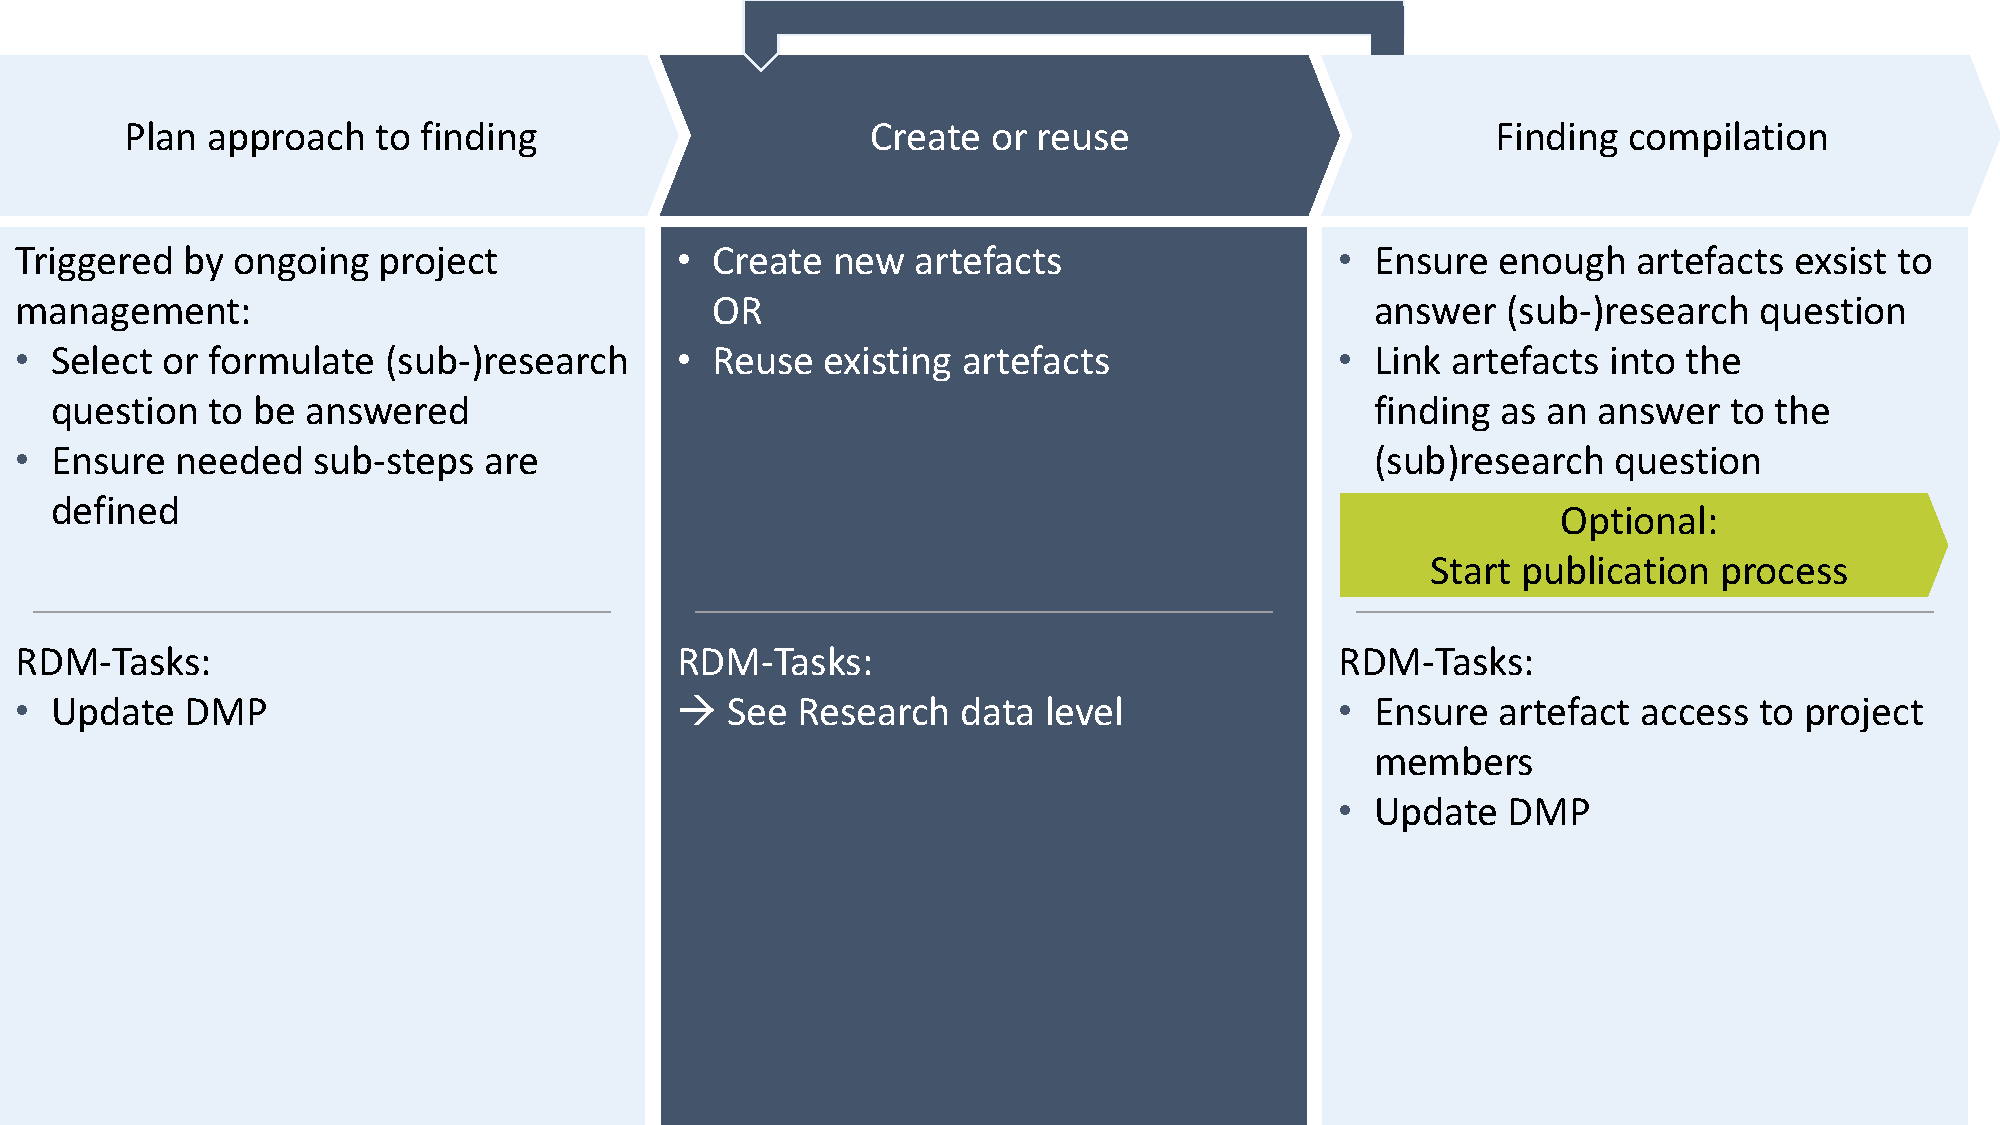
\includegraphics[trim={0 4.7cm 0cm 0cm}, clip, width=\textwidth]{figures/Mid_level_v3.pdf}
    \caption{The redesigned finding level of the proposed research process}
    \label{fig:Mid_level_redesign}
\end{figure}



\subsection{Feedback on the research data management level}
\label{LowFeedback}

On the \ref{Glossary:research data management level}, interviewees mostly agreed.
Their biggest concerns were clustered at the \textit{\ref{Glossary:check}} step.
This can also be seen in figure \ref{fig:DescriptiveFeedback_low}.

\begin{figure}[ht]
    \centering
    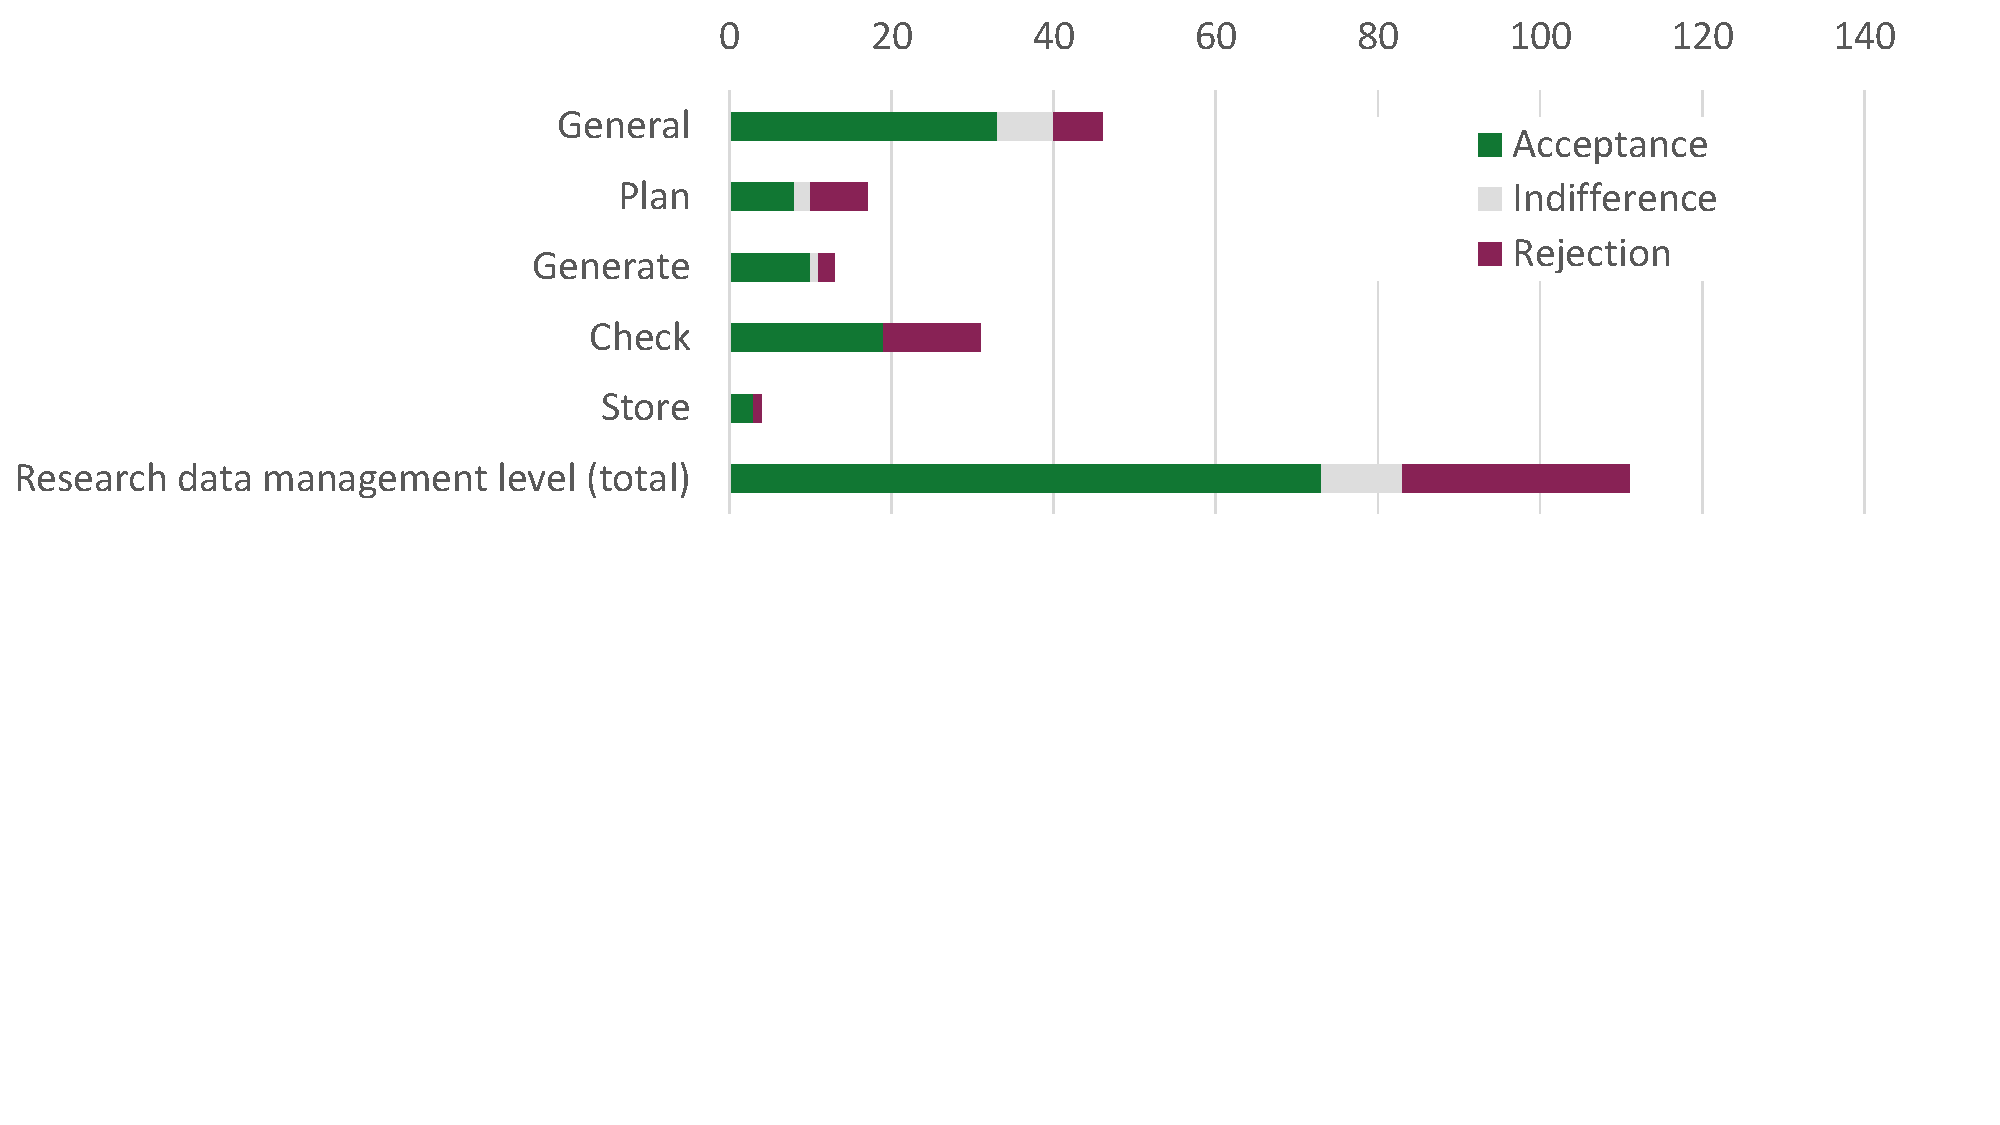
\includegraphics[trim={0cm 10.25cm 0cm 0cm}, clip, width=\textwidth]{figures/Table5_Figure.pdf}
    \caption{Codes on the feedback received on the research data management level. The exact numbers can be found in table \ref{tab:DescriptiveFeedback_low} in the appendix.}
    \label{fig:DescriptiveFeedback_low}
\end{figure}

% General - Done
%\todo[inline]{Überlegen: Rückkopplung Low level zu high level}
%\todo[inline]{Quality gates auf top level! ggf auch auf mid und low?}
%\todo[inline]{Ist Low Level Iterativ, oder ist nur Mid Level Iterativ?}

The wording was adjusted to fit the \ref{Glossary:finding level}.
As the \ref{Glossary:research data management level} is focussed on the generation of \ref{Glossary:artefact}s, it is renamed to \ref{Glossary:artefact level}.

The \ref{Glossary:artefact level} happens to be of a very short nature in general, compared to the duration of work packages, as most activities can be completed within a few hours.
Yet, the generation of data may take up to days or even weeks depending on the setup.
The tasks performed by researchers are able to be performed and finished immediately and without accompanying activities.
Hence, the \ref{Glossary:artefact level} is not iterative, but straight forward.
Once performed, the outcome is either \ref{Glossary:store}d or deleted. 
In both cases the result is taken to the \ref{Glossary:finding compilation} to consider if more \ref{Glossary:artefact}s need to be \ref{Glossary:generate}d or the new knowledge generated is sufficient to answer the research question.


% L1  - Done
%\todo[inline]{: In Paper: M1 und L1 sind Abgleich zu T1 -> Reaktion auf Änderungen, gehört zu T2 ongoing project management}
%\todo[inline]{Richtige Planung muss sehr klein sein}
%\todo[inline]{Ich weiß gar nicht genau gefühlt. Es sind hier noch weitere Tasks bei Plan aber bin ich jetzt gerade nicht so sicher. Bzw. Ja, also ich überlege jetzt einfach nur was sind das für Artefakte, die da rauskommen? Was sind das für Arten von Datenerhebung? So. Also im Wesentlichen ich ich störe mich jetzt gerade nur ein bisschen an dem Wording. Nicht weil es falsch ist, sondern weil es halt irgendwie, glaube ich, mehr meint, als es irgendwie artikuliert. Gerade bei General Use. Previous Artefakts input generate gather or process data Genau. Und dann record meta data along with data generation.}
%\todo[inline]{Es wird nicht dokumentiert, was als input verwendet wurde, aber es wird schom geguckt, was verwendet wird}
In the \ref{Glossary:preparation} phase of the data generation, the wording is adjusted to fit the actual scope of the step, namely the \ref{Glossary:generation setup}.
The data generation is set up, meaning that the exact procedure of data generation is planned and \ref{Glossary:check}ed. This, for example might be the inspection of a test bench, if all cables are connected correctly and if the software is set up correctly for the recording of data.
For interviews, this might also be the \ref{Glossary:check} if the recording devices are running properly, the interview guideline is present and known to the interviewers.
Furthermore, input \ref{Glossary:artefact}s are selected.
This step happens moments before the generation of data.

% L2
%\todo[inline]{Daten und ich analysiere Daten und deswegen also irgendwie so dieses du müsste man vielleicht noch mal unterteilen bzw DO und ACT gibt es ja irgendwie auch so, da müsste man vielleicht sich mal  Gedanken machen, ob dieses Generate nicht irgendwie noch mehr  beinhaltet. Vielleicht.}
%\todo[inline]{Was beinhalten die automaisch aufgenommenen metadaten?}
Then data is \ref{Glossary:generate}d.
Ideally, metadata is automatically recorded with data generation.
This might encompass environmental conditions, labels for data or demographic data.
The form of metadata to be used is highly dependant on the subject of investigation and the (sub-)research question to be answered.

% L3 - Done
%\todo[inline]{Daten und ich analysiere Daten und deswegen also irgendwie so dieses du müsste man vielleicht noch mal unterteilen bzw DO und ACT gibt es ja irgendwie auch so, da müsste man vielleicht sich mal  Gedanken machen, ob dieses Generate nicht irgendwie noch mehr  beinhaltet. Vielleicht.}
%\todo[inline]{Wording validity, Inhalt der Aussage nicht nutzen, weil zu unklar}
%\todo[inline]{Vergleich Praxis und Theorie: Check wird oft vergessen}
%\todo[inline]{Validtty is not always done}
%\todo[inline]{Gelöscht wird meistens nichts}
%\todo[inline]{We usually try to find out why this sensor malfunctioned at that time}
%\todo[inline]{Forschende wollen nichts löschen und hoffen auf gelegenheit zur verwertung der schlechten daten}
%\todo[inline]{Tatsächlich hat es auch ein solcher Datensatz in Anführungsstrichen ein fehlerhafter Datensatz in meine Dissertation geschafft, weil ich anhand dem ein Phänomen erklärt habe, quasi was also im Prinzip das, was ich gemacht habe.}
%\todo[inline]{Loop delete zu rück zu Planning}
Afterwards, the data is \ref{Glossary:check}ed for correct recording, i.e. correct set up of the data generation.
So this step is not a validation of data but \ref{Glossary:ensure}s data correctness.
Although interviewees stated that this step was often not performed, we recommend it highly to filter out unusable data right away.
If the data is corrupted in any way, e.g. a sensor was not connected or malfunctioned, the data can be deleted, because no information can be drawn from this failed data generation.

% L4 - Done                             
%\todo[inline]{17. - s. store und ensure + L4+M3}
%\todo[inline]{Hier optional schonmal teammitgliedern zur verfügung stellen}
%\todo[inline]{Ordentliches Ablegen ist noch nicht im intuitiven handeln angekommen}
%\todo[inline]{Store kann auch schon sein, Daten so zu storen, dass die anderen zugriff haben}
If the data was recorded correctly, it can be \ref{Glossary:store}d along with the corresponding metadata.
The \ref{Glossary:artefact} should be \ref{Glossary:store}d in a location that is backed up and ideally offers access to \ref{Glossary:project} members.
The updated \ref{Glossary:artefact level} is shown in figure \ref{fig:Lowlevel_redesign}.


\begin{figure}[htbp]
    \centering
    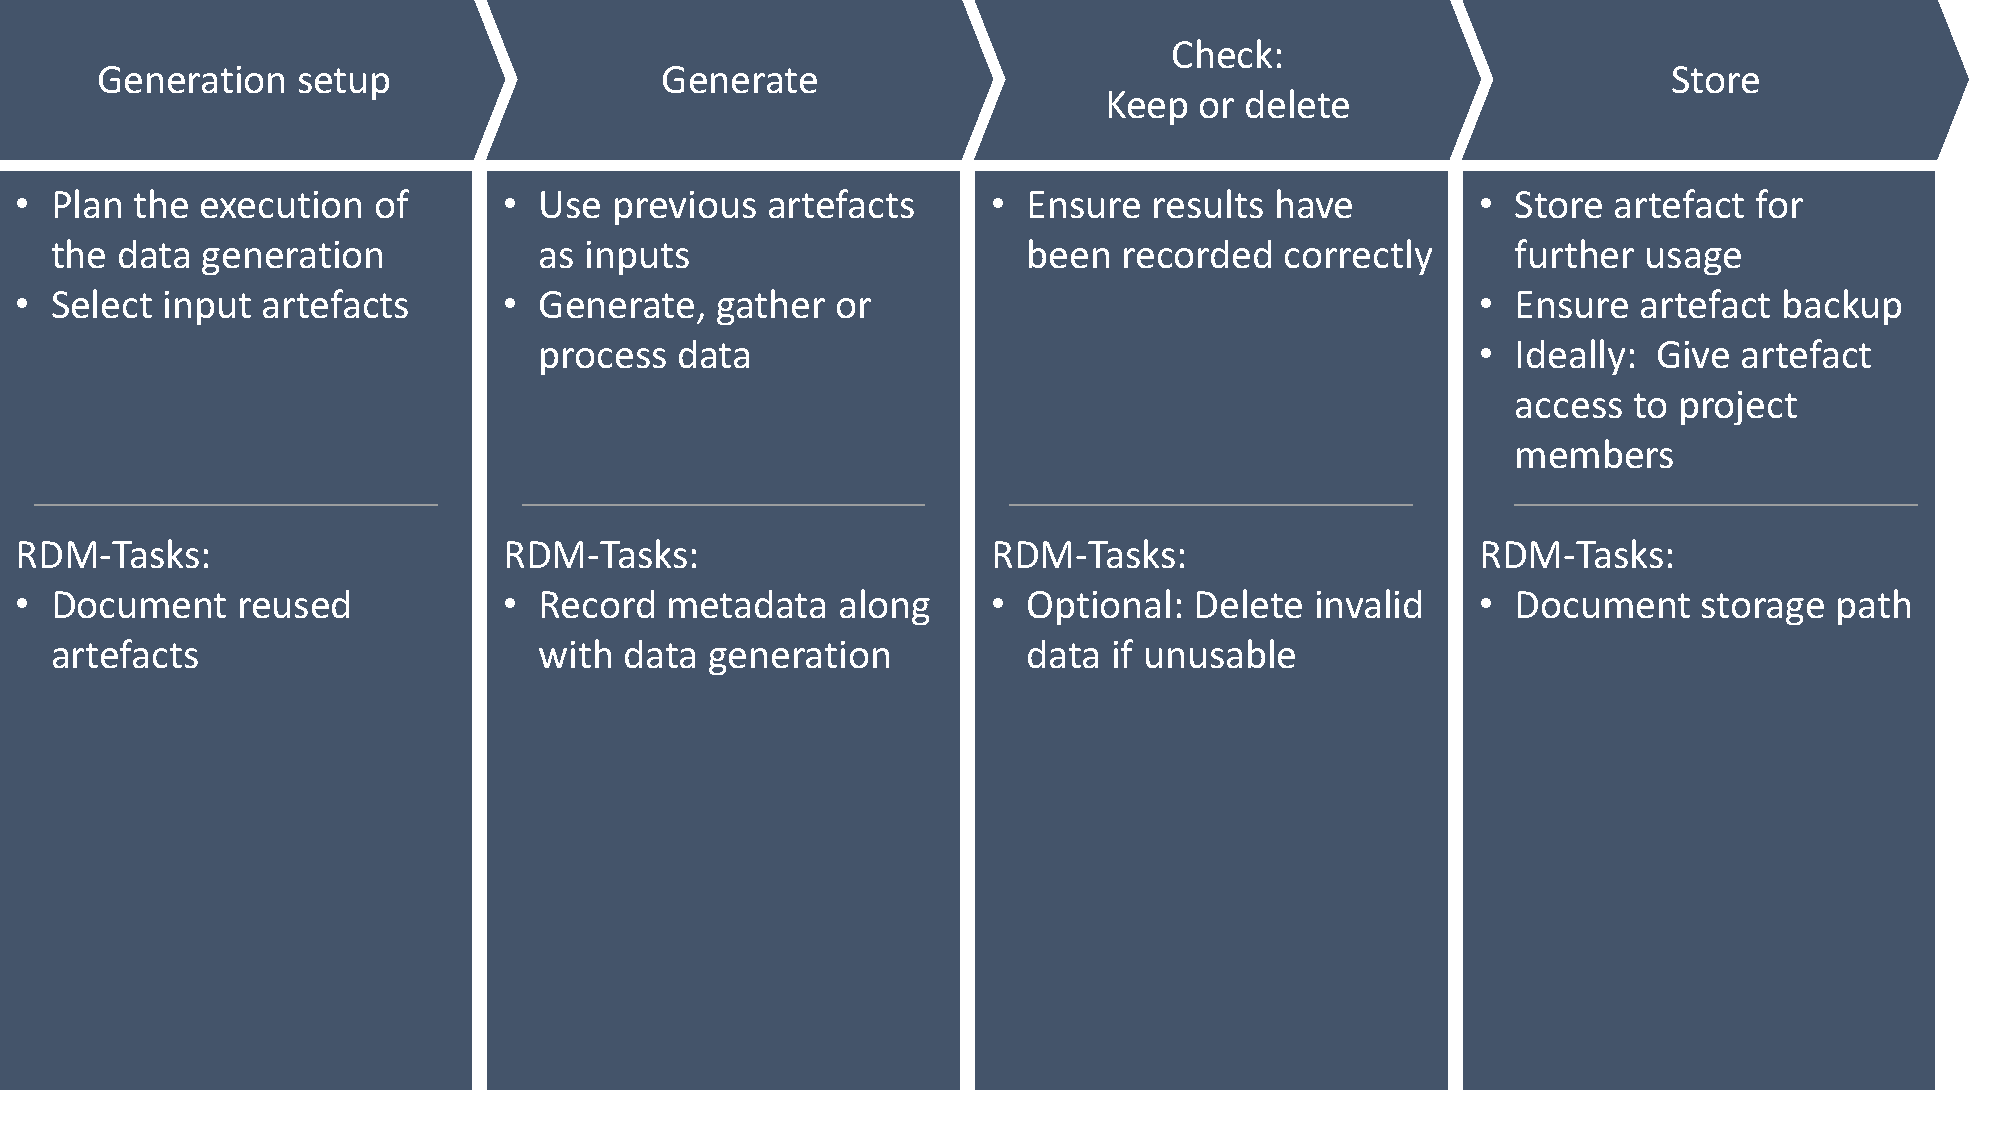
\includegraphics[trim={0 7.2cm 0 0cm}, clip, width=\textwidth]{figures/Low_level_v2.pdf}
    \caption{The redesigned research data management level of the proposed research process}
    \label{fig:Lowlevel_redesign}
\end{figure}

%\afterpage{\clearpage}

\subsection{Feedback on publication workflow of the process}
\label{PublicationFeedback}

%\todo{Das passt hier nicht mehr schön rein, habe schon genug Zitate. Gerade aber den ersten Satz finde ich total gut. Vielleicht können wir das noch woanders einbauen.}

%\hfill\begin{minipage}{\dimexpr\textwidth-0.5cm}
 %   \textit{
  %      \enquote{
   %         In mechanical engineering, reality means: 
    %        publish, publish, publish. 
     %       It's different in other academic disciplines. 
      %      [...] 
       %     We have \ac{dfg} proposals that state you must produce two publications per employee per year. 
        %    So there's definitely a certain amount of pressure.%LUH
        %}
    %}
%\end{minipage}

The interviewees generally found the \ref{Glossary:publication process} to be appropriate. 
Nevertheless, comments such as \enquote{\textit{[the publication process] basically depicts reality as it is and should be}}
%\todo{Wir müssen uns auch mal überlegen, ob wir die Zitate immerhin als "Person 1" oder so kennzeichnen. Macht es immerhin transparenter, dass nicht alle Aussagen von einer Person kommen. Generell auch: kennzeichnen wir die kursiv, längere Zitate mit breiterem Seitenrand oder so?} %Uni Stuttgart
illustrate the discrepancy between theory and practice. 
For this reason, isolated differences to the model process emerged several times in the interviews. 
They can be attributed to time pressure and external factors (such as \ref{Glossary:project} partners or funding regulations) in day-to-day research.
Figure \ref{tab:DescriptiveFeedback_pub} shows how this feedback was distributed over the proposed phases.

\begin{figure}[ht]
    \centering
    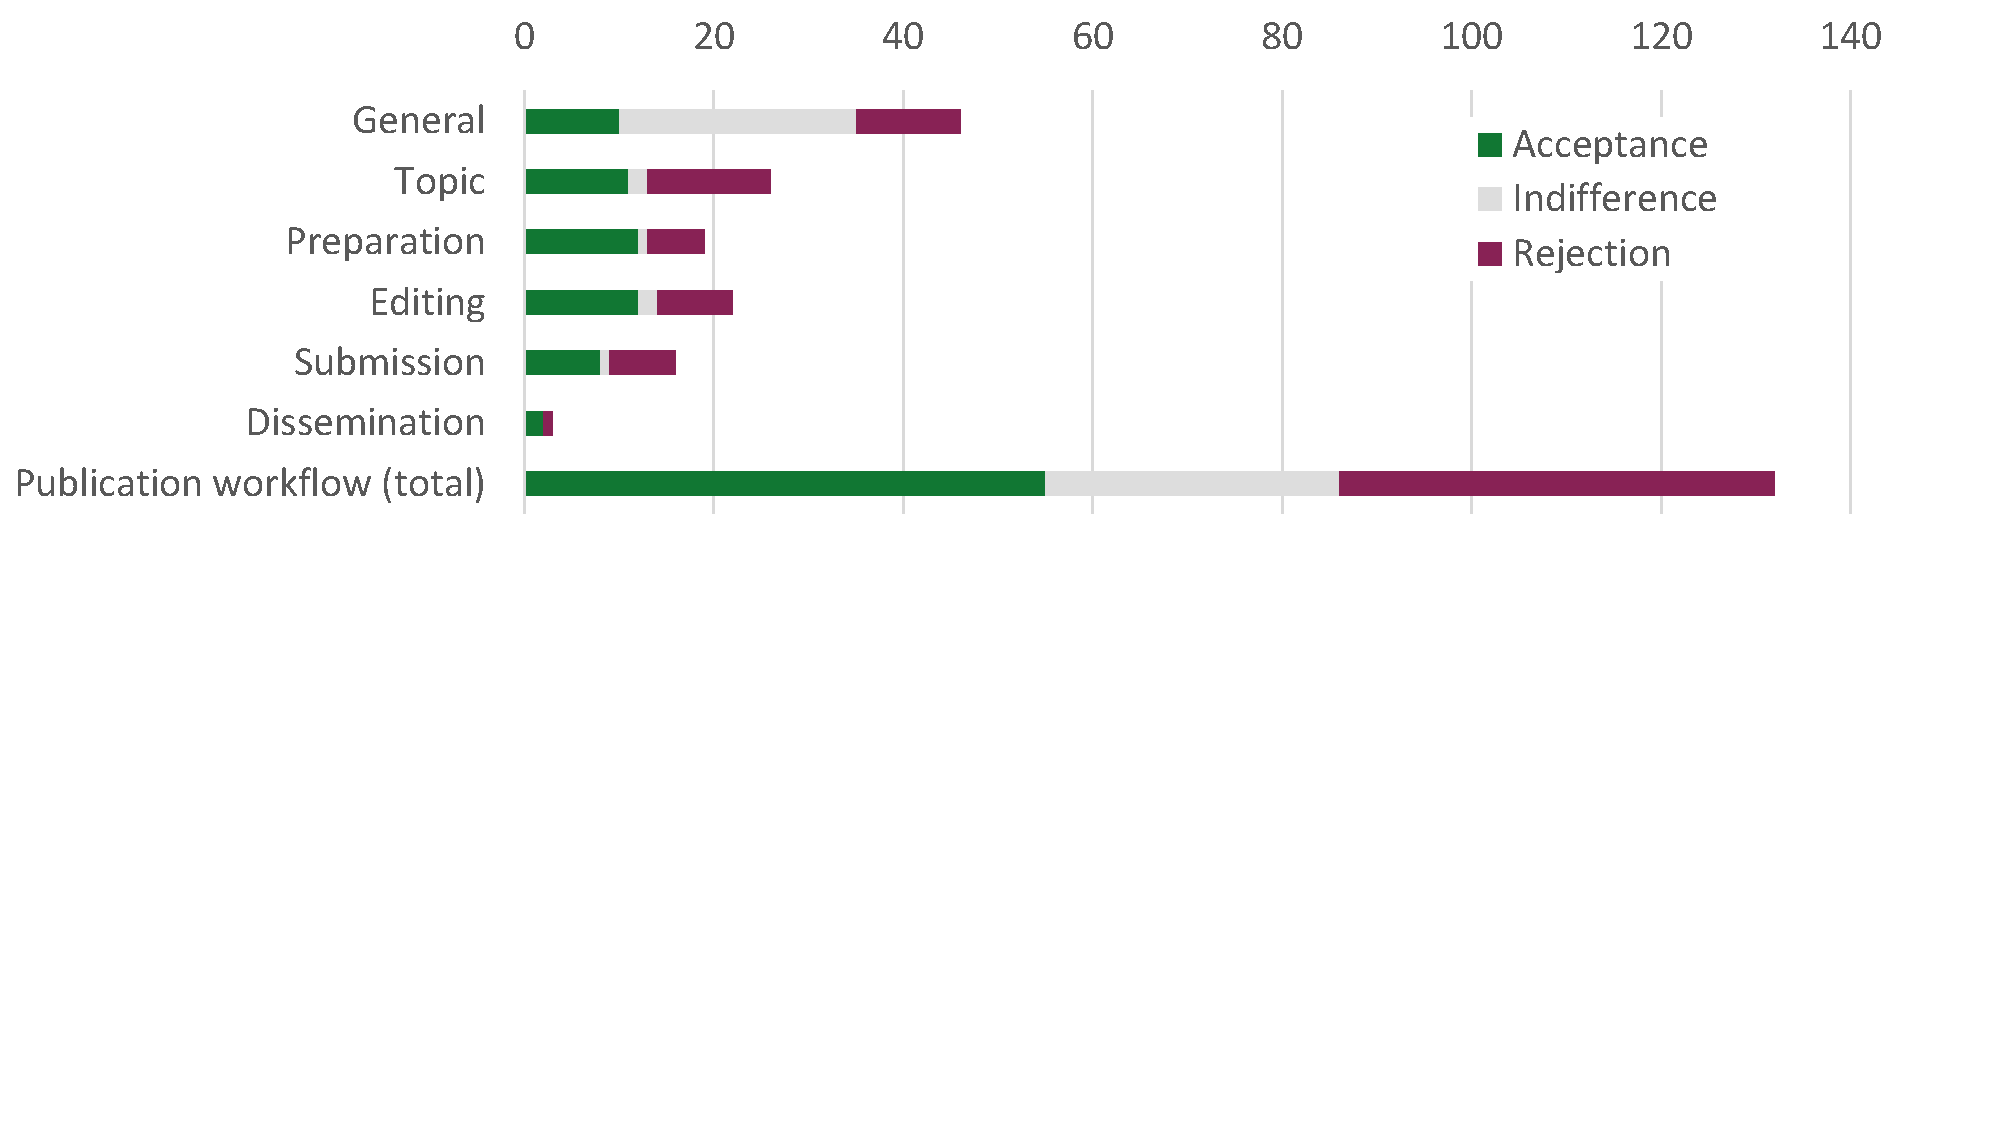
\includegraphics[trim={0cm 10.25cm 0cm 0cm}, clip, width=\textwidth]{figures/Table6_Figure.pdf}
    \caption{Codes on the feedback received on the publication workflow. The exact numbers can be found in table \ref{tab:DescriptiveFeedback_pub} in the appendix.}
    \label{fig:DescriptiveFeedback_pub}
\end{figure}

% General
%\todo[inline]{Unterscheidung zwischen Science und Scholarly Communication, Grafik zweiteilen}
%\todo[inline]{Prepreints berücksichtigen}
%\todo[inline]{Publikationsprozess kann parallel zur Forschung laufen}
%\todo[inline]{Im Paper: Concept Paper als Beispiel}
%\todo[inline]{Praxis vs. Theorie: Auswahl des Journals, Zeitpunkt}

% P1
%\todo[inline]{Topic: + Scoping (inhaltlich, Abstract); P2:hat Fokus auf formal}
%\todo[inline]{Interne und externe Trigger für Publikationsprozess}
%\todo[inline]{Externer Publikationstrigger}
%\todo[inline]{Extrinsischer Trigger für Publikation}
%\todo[inline]{Extrinsischer Trigger für Paper}
%\todo[inline]{Intrinsische vs. extrinsische Publikationstrigger}


% P2
%\todo[inline]{P2: (externe) Vorgaben für Veröffentlichungen berücksichtigen}
Evaluating the first two phases, a need for a clearer distinction has emerged: 
While the \ref{Glossary:preparation} phase sets formal framework conditions, the focus in the \ref{Glossary:topic} phase is on planning the content. So they are renamed to \ref{Glossary:topic and scoping} and \ref{Glossary:formal preparation}. 
In addition, a \ref{Glossary:publication} is not only triggered by the \ref{Glossary:finding compilation}, as previously stated. 
In practice, there are two types of triggers:
\begin{itemize}
    \item \hyperref[Glossary:self-motivated publication trigger]{Self-motivated publication trigger}s, e.g.: intrinsic motivation of researchers to share a \ref{Glossary:finding} that they have compiled; gaining an overview of the state of the art in the context of a review paper; turning a thesis into a paper together with the student
    \item \hyperref[Glossary:externally motivated publication trigger]{Externally motivated publication trigger}s, e.g.: invitations to conferences and associated deadlines; finalising the \ref{Glossary:publication} plan from the \ref{Glossary:project} proposal; doctoral degree regulations; writing a cumulative dissertation; supervisors push for \ref{Glossary:publication}
\end{itemize}

% P3
%\todo[inline]{P3+P4: Rückkopplung expliziter darstellen, wegen Peer Review}\todo{Das habe ich in der Grafik extra betont. Reicht das?}
%\todo[inline]{P3: internes Review}
%\todo[inline]{P3: interner Freigabeprozess}

% P4
%\todo[inline]{P3+P4: Rückkopplung expliziter darstellen, wegen Peer Review}

% P5
\iffalse
\begin{table}[ht]
    \begin{tabularx}{\textwidth}{X|X}
        % \toprule
        \textbf{Internal triggers} & \textbf{external triggers} \\
        \toprule
        intrinsic motivation of researchers to share a \ref{Glossary:finding} that they have compilated & invitations to conferences and associated deadlines  \\
        gaining an overview of the state of the art in the context of a review paper &  finalising the \ref{Glossary:publication} plan from the \ref{Glossary:project} proposal \\
         turning a thesis into a paper together with the student &  doctoral degree regulations demand \ref{Glossary:publication}s  \\
          &  writing a cumulative dissertation  \\
        &  supervisors push for \ref{Glossary:publication}  \\
        % \hline \hline
        % &&            Sum: & \\
    \end{tabularx}
    \caption{Internal and external triggers for publications}
    \label{tab:TriggersPublication}
\end{table}
\todo{Findest du die Darstellung als Bulletpoint List oder als Tabelle besser? Hängt ggf. auch vom verfügbaren Platz ab}
\fi

Even if there are various triggers for \ref{Glossary:publication}s, it remains clear that \ref{Glossary:finding compilation} is essential for this process: 

\hfill\begin{minipage}{\dimexpr\textwidth-0.5cm}
    \textit{
        \enquote{
            Let me put it this way: 
            If I don't have any findings, then it will be difficult [...] writing a publication. 
            But of course I can try to make findings possible in a more targeted and less targeted way. 
            You know exactly that some things might work and then you do something in that direction, because you know that if you do this or that, then I will at least manage to generate enough new knowledge to at least justify a publication. 
            (...) 
            At the end of the day, of course, it would be nicer if I had a specific research question that I try to answer or was trying to answer and then say: 
            Hey, now the research question has been answered and now I'm going to write a publication about it. 
            Yes, there are – in practice, I would say there are both.
        } %Uni Stuttgart
    }
\end{minipage}


This description fits with interviewees' statements, that writing \ref{Glossary:publication}s is a reflective activity, where \ref{Glossary:research data} and text production are closely linked.
When converting \ref{Glossary:artefact}s and \ref{Glossary:finding}s into a written form (to create a medium that passes on the knowledge from the \ref{Glossary:finding compilation} to other people), gaps may become visible that need to be filled with additional content, or new contexts may emerge.

\hfill\begin{minipage}{\dimexpr\textwidth-0.5cm}
    \textit{
        \enquote{
            I always find that it all makes a lot of sense in my head. 
            But it's only when you put it down on paper that you realise: 
            Oh no, that's somehow, there's no thread running through it. 
            So that's actually always a point where you have to think more deeply about it when you're writing what have you actually just done here, because you have to get your own thoughts down somehow, and so there's a lot of reflection involved.
        } %LUH
    }
\end{minipage}

At the same time, the interviewees emphasised that there are also \ref{Glossary:publication} types such as concept papers that contain less data.
Interviewees stated that \ref{Glossary:publication}s could occur at any time over the course of the whole \ref{Glossary:research project}.
%\todo{Referenz zu "Publikationen über den ganzen Forschungsprozess hinweg?}
Another aspect that the interviewees repeatedly mentioned was preprints: 
By publishing \ref{Glossary:publication}s that have not yet been peer-reviewed, they want to position themselves quickly in the dynamic academic discourse and make their work referencable so that they can be followed up in subsequent \ref{Glossary:publication}s.

Finally, the interviewees addressed the communication of scientific results to the public - usually referred to as \enquote{\ref{Glossary:science communication}} - which is becoming increasingly established in the job description of researchers \cite{Konneker.2012}.
Communication within the scientific system is correspondingly \enquote{\ref{Glossary:scholarly communication}}. (cf. e.g. \cite{Hagenhoff.2007}, \cite{Burns.2003}) 
Since these two sub-areas of publishing differ in terms of target group and communication goal and form, but are similar looking at the basic process, the revised graphic is divided into two parts, as shown in figure \ref{fig:Publication_redesign}. 

\begin{figure}[htbp]
    \centering
    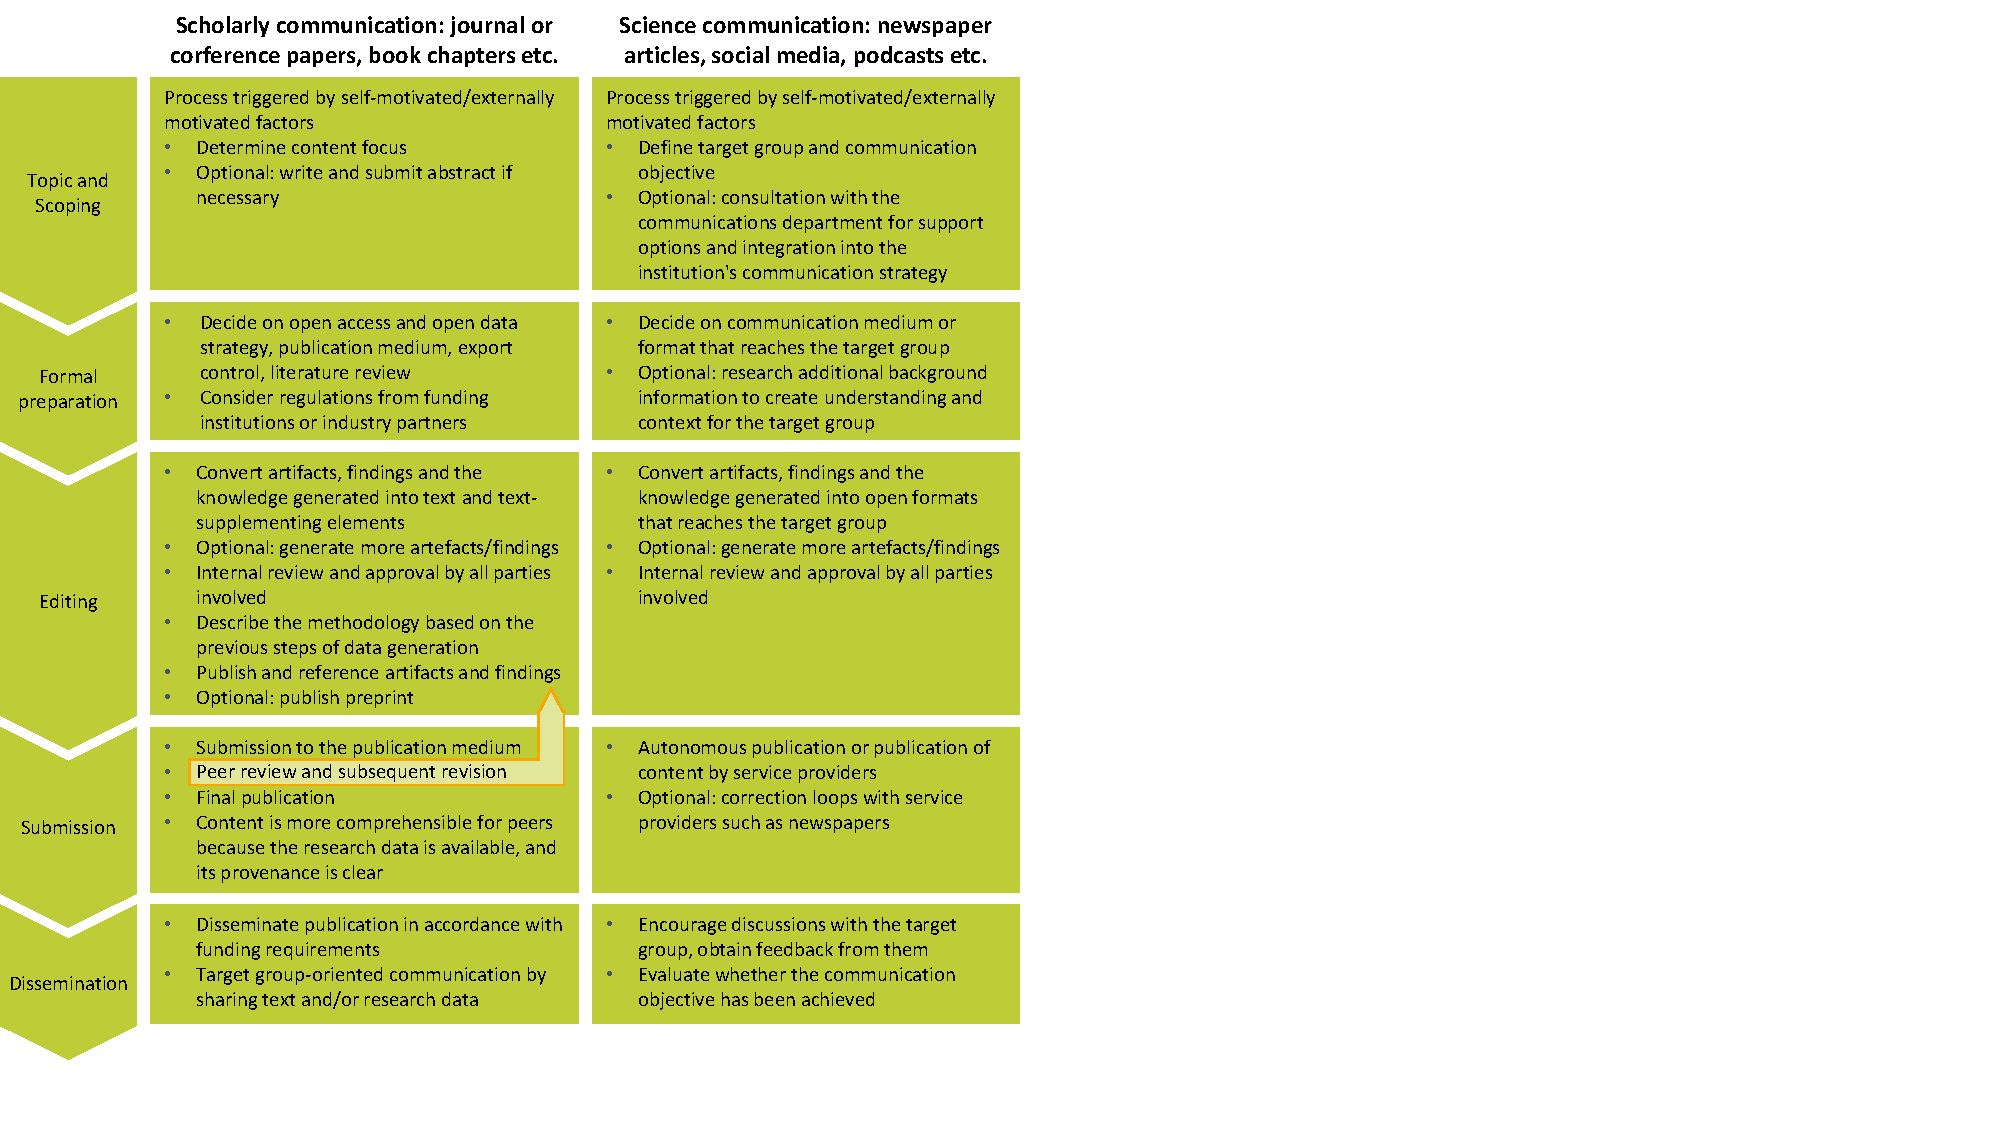
\includegraphics[trim={0 1cm 16.5cm 0}, clip, width=\textwidth]{figures/Publication_v7.pdf}
    \caption{The redesigned publication process}
    \label{fig:Publication_redesign}
\end{figure}

The content on \ref{Glossary:science communication} is essentially based on the explanations of Konneker \cite{Konneker.2012}, Frick and Seltmann \cite{Frick.2024} and Bertemes et al. \cite{Bertemes.2024}.
A key difference between \hyperref[Glossary:science communication]{science} and \ref{Glossary:scholarly communication} lies in the support.
Depending on the involvement of the respective institution's communication department, process steps in the area of \ref{Glossary:science communication} (e.g. parts of \ref{Glossary:editing} or \ref{Glossary:submission}) are handled by the department rather than by the researchers themselves - in contrast to \ref{Glossary:scholarly communication}.

In addition to the highlighted aspects so far, the \ref{Glossary:publication process} has undergone further minor adjustments, such as the addition of internal reviews and (external) approval processes. 
%Figure \ref{fig:Publication_redesign} shows the revised graphic.\todo{Referenz auf neue Grafik}


%"Well, if you're publishing journal articles now, then... [...] You go through the review process, and ideally, it's accepted after two or three rounds. [...] We simply have a process that, so to speak, modifies the research result again.[...] Sometimes I also have to revise things and go back to my data. And often, you add something again or something like that." %TU Berlin



%"Research and publishing is really about trying to describe the findings you have and put them into written form, and so on. But for us, it's often also the case that this process leads to discovering new research questions where further work is needed. Like, I’m missing data there. That might not be entirely conclusive yet, so it would need to be investigated again." %LUH

%\todo[inline]{Extrinsische Trigger für Publikation: Publish or Perish}



\subsection{Overall process}
The overall process was met with general approval by the interviewees.
Still, the refinements made to the process on the basis of the interviewees feedback improved it significantly.
Wordings have been specified, steps and tasks have been made more explicit and the structure of the process was adapted to the reality of research while also upholding standards of \hyperref[Glossary:research data management level]{\ac{rdm}}.
The final process is depicted in figure \ref{fig:Levels_redesign}.

% \afterpage{\clearpage}

\begin{figure}[htbp]
    \centering
    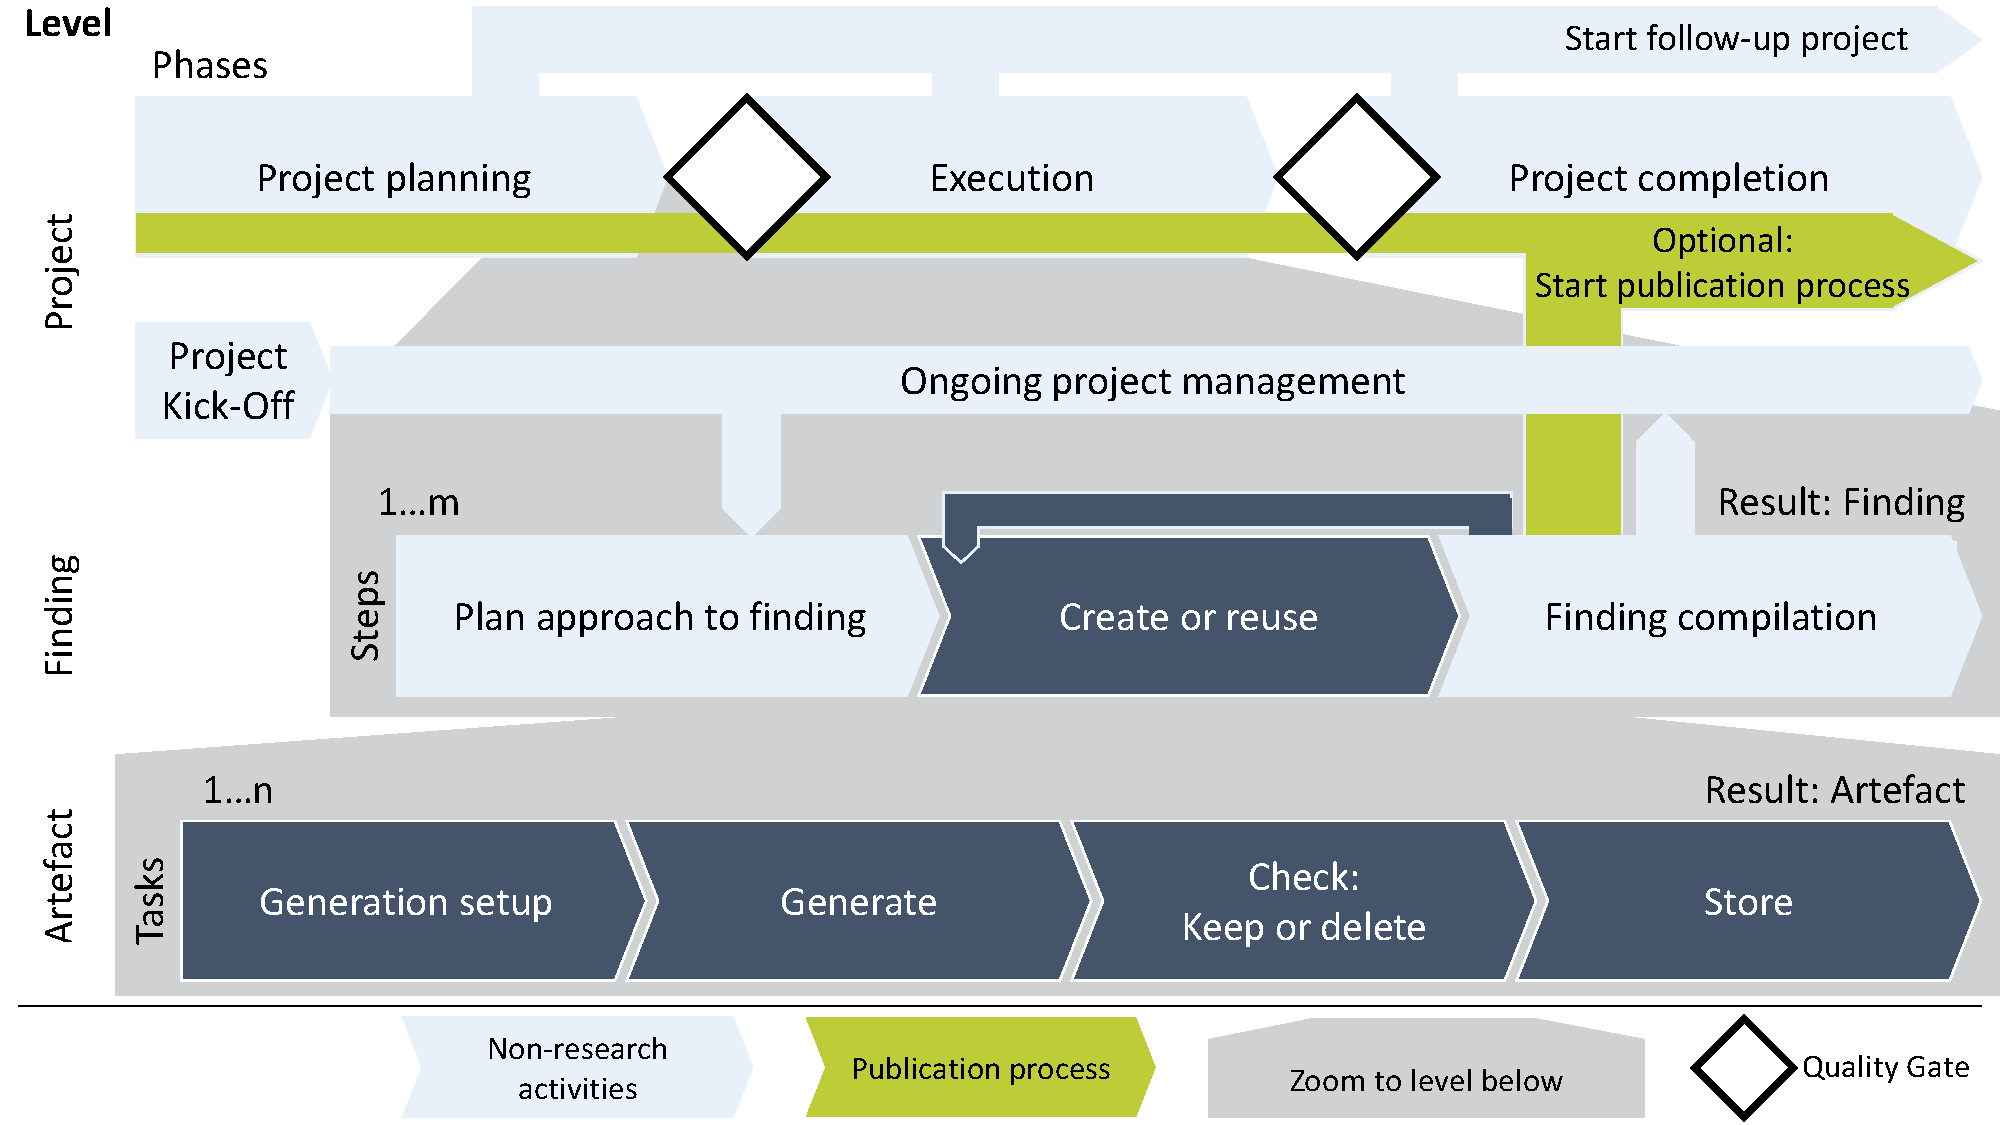
\includegraphics[trim={0 0cm 0cm 0cm}, clip, width=\textwidth]{figures/Levels_v7.pdf}
    \caption{General structure of the proposed \hyperref[Glossary:research data management level]{\ac{rdm}} process}
    \label{fig:Levels_redesign}
\end{figure}

%\FloatBarrier 

In comparison to figure \ref{fig:Levels}, the biggest changes are:

\begin{enumerate}[noitemsep]
    \item The option to start follow-up \ref{Glossary:project}s in any of the process' phases%\todo{@TH: Neuer Gedanke: Muss es immer ein follow-up project sein? Das ist für mich eher etwas nachgelagertes. Wenn aber aus dem Projekt noch Dissen und Abschlussarbeiten z. B. entstehen, die darauf einzahlen, sind das eher Sidekick-Projekte. Habe im Kopf ein Bild von mehreren Branches in Git. Oder sind das eher Arbeitspakete?}
    \item The option to start a \ref{Glossary:publication process} in any of the process' phases
    \item The option to \ref{Glossary:generate} \ref{Glossary:finding}s in the \ref{Glossary:project planning} phase
    \item The \ref{Glossary:project kick-off} was moved to not be included in the \ref{Glossary:content-wise execution} and instead precede the ongoing project management.
    \item A feedback loop between \ref{Glossary:finding compilation} and \ref{Glossary:plan approach to finding}
    \item A feedback loop between \ref{Glossary:finding compilation} and \ref{Glossary:create or reuse}
    \item Wording changes, especially on the names of the levels:
    \begin{itemize}
        \item \hyperref[Glossary:project management level]{Project management level} changed to \ref{Glossary:project level} 
        \item \hyperref[Glossary:work package level]{Work package level} changed to \ref{Glossary:finding level} 
        \item \hyperref[Glossary:research data management level]{Research data management level} changed to \ref{Glossary:artefact level} 
    \end{itemize}
\end{enumerate}

This process validated the previously identified needs, demands, and practices of researchers from engineering sciences.
It aims to resemble the day-to-day research activities of researchers in engineering sciences as best as possible while also integrating \hyperref[Glossary:research data management level]{\ac{rdm}} activities as seamlessly as possible.


\iffalse
\subsection{bisher nicht berücksichtigt}


\todo[inline]{Rauslassen? RDM ist service task der die anderen ebenen absichert --> Rückkoplung zu Projektmanagement}
\todo[inline]{Rauslassen? Prozess is auf open science ausgerichtet, das geht bei industrie aber nicht so einfach}



\paragraph{Nicht berücksichtigt bisher in Top}
\todo[inline]{: In Paper: M1 und L1 sind Abgleich zu T1 -> Reaktion auf Änderungen, gehört zu T2 ongoing project management}
\todo[inline]{Überlegen: Rückkopplung Low level zu high level}
\todo[inline]{Nochmal eine Ebene mehr zwischen top und mid für sehr große projekte --> Projekte die parallel laufen}
\todo[inline]{Für Text: Rückkopplung zu Finding planning durch Quality gate, ob goal erreicht}
\todo[inline]{Content wise Execution prägnanter darstellen}
\todo[inline]{wenn Projekt verlängert wurde, dann ist die completion nicht so strikt zu sehen}

\paragraph{Nicht berücksichtigt bisher in mid}
% Nicht verwendet - MID 
\todo[inline]{Wenn man eine Publikation schreibt (bzw. finding generiert???), dann nimmt man nochmal alles zusammen, und denkt kritisch drüber nach. das kann auch neue zkylen triggern !!!! Rückkopplung finding planning zu finding compilation}
\todo[inline]{2.6. Wording: Gerade bei General Use. Previous Artefakts input generate gather or process data Genau. Und dann record meta data along with data generation.}
\todo[inline]{Artefakte früher team members bereitstellen? -> Ensure vs ???}
\todo[inline]{Archiving schon oft teil von T2}
\todo[inline]{Deswegen finde ich das schon ganz, ganz treffend, dass es so vor dem oder beim Schreiben von Veröffentlichungen noch mal so einen Peak gibt, wo immer mehr Forschungsergebnisse erstellt werden als vorher.}
\todo[inline]{Arbeitspakete sind nie abgeschlossen, sondern genügen dem antrag}
\todo[inline]{17. - s. store und ensure + L4+M3}

\paragraph{Nicht berücksichtigt bisher in low}


\paragraph{Nicht berücksichtigt bisher in pub}

\fi

\section{Discussion and Limitations}
\label{Discussion}

% Evidenz ist hoch
The answer to the research question can be given with a high certainty.
The evidence for this statement is high, as it is
based on the consolidation of 
eight problem-centred interviews with 19 researchers, 
the surveying of 13 research \ref{Glossary:project}s by another eight researchers on their workflows
and this validation with another ten researchers in expert interviews.
This total of 37 different researchers questioned on their research's demands and structure.

% Bias zu beginn
While the first two methods were biased on the \ac{rwth} and \ac{luh}, the validation took into consideration the whole \ac{tu9}.
While, smaller universities or universities of applied sciences might have different approaches to research, the approach of validation via \ac{tu9} allows for insights into a big part of engineering sciences.

% Changes sind klein und alle AUssagen gehen in ähnliche Richtung
Furthermore, the changes and adaptions to the process, while seemingly big, are not crucial.
The biggest changes were made due to wording inconsistencies.
Certain parts of the process were explicated and defined more precisely, or in some cases, more openly to allow for a better situational fit.
The overall process structure with its levels and their contents remain unchanged.

% Rückbezug erstes Paper
The validation, which was urgently missing in the last paper, was now performed.
It confirmed the good reception the process got in several events where it was presented (see \cite{Hamann.2022,Hamann.2023,Hamann.2023b,Hamann.2023c}).
Overall, it affirmed the process with minor changes made to it.

Nevertheless, the methods used should be critically contextualized: The usual quality criteria such as objectivity, reliability and validity in the sense of definitions from natural sciences can only be applied to expert interviews to a limited extent. For example, the interviews themselves take place in social situations that create a dynamic between interviewers and interviewees or even unintentional mutual influences, which can lead to bias. \cite{Bogner.2014} The objectivity of qualitative content analyses - a method which core is the interpretation of the material by people with different knowledge and views - can at least be strengthened by instruments such as intercoder analysis. \cite{Mayring.2022}

\section{Conclusion and Outlook}
\label{Conclusion and Outlook}



In this article, we validated our proposed process for \ref{Glossary:project}-oriented \hyperref[Glossary:research data management level]{\ac{rdm}} in engineering sciences.
This process, now called \acl{prorp} (\ac{prorp}), is the result of a thorough investigation of the problems, requirements, workflows and practices of engineering researchers.
In total 37 different researchers were consulted by the means of different methods.

\ac{prorp} is validated in this article by a series of ten expert interviews.
The result is a validated process that received minor adjustments to better fit the reality of day-to-day work and facilitate understandability.
This also leads the the answer to the proposed research question:

\hfill\begin{minipage}{\dimexpr\textwidth-0.5cm}
    \textit{
        \textbf{
            Can our proposed \hyperref[Glossary:research data management level]{\ac{rdm}} process be deployed into engineering research projects?
            \newline
            With the changes made to it, yes.
        }
    }
\end{minipage}


\ac{prorp} will provide the foundation of Jarves, the Joint Assistant for Research in Versatile Engineering Sciences \footnote{\url{https://jarves.nfdi4ing.de/}}. 
This digital data steward guides engineering researchers in their \hyperref[Glossary:research data management level]{\ac{rdm}} throughout their whole research \ref{Glossary:project}. 
Jarves will also contain the management of \hyperref[Glossary:research data management level]{\ac{rdm}} guidelines within a decision support system.
\cite{Hamann.2024b} %HAMA24d
Jarves was validated by a Proof-of-Concept-Study in a real world application by Hamann et al. \cite{Hamann.2025b}.

\ac{prorp} offers a missing link between theoretical \hyperref[Glossary:research data management level]{\ac{rdm}} and actual research practices.
It offers a bridge between research \ref{Glossary:project}s and their structure and the life cycles of \ref{Glossary:research data}.
We hope, that \ac{prorp} facilitates the application of \hyperref[Glossary:research data management level]{\ac{rdm}} in engineering sciences.
Additionally, in future research \ac{prorp} could be transferred to other disciplines that utilize \ref{Glossary:project}-oriented research.




%\newpage


% \iffalse
 \iftrue

\appendix

\section{Appendix}
\label{Appendix}

This appendix contains a glossary on the most important terms in this paper and the process it describes as well as further elaborations on the exact numbers of codes for each level of the process.

%\subsection{Glossary} 
\subsection{Glossary}
\label{Glossary}


This glossary aims to facilitate understandability for those who would like to implement, utilise or further develop this process.
The glossary is an updated version of the previous paper's glossary. \cite{Hamann.2024b}

%\begin{table}[h!]
%\centering
\begin{longtable}{ p{0.3\textwidth}  p{0.7\textwidth} } 
    \textbf{Analysed data}
    \tablelabel{analysed data}{Glossary:analysed data}
    & 
    Any \ref{Glossary:data} that is processed in any way that allows for new information to be derived from it. \textbf{On \ref{Glossary:artefact level}. Straight forward.}\\
    \midrule
    \textbf{Artefact}
    \tablelabel{artefact}{Glossary:artefact}
    \tablelabel{Artefact}{Glossary:Artefact}&
    The result of one iteration of the \ref{Glossary:artefact level}. An \ref{Glossary:artefact} is planned, contextualised and validated \ref{Glossary:research data} in its smallest unit. It may be a primary data collection or the implementation of source code. It was generated by creating a \ref{Glossary:generation setup}, generating the data and performing a check to \ref{Glossary:ensure} the correct recording and, if valid, storing the data. An artefact is information. \textbf{On \ref{Glossary:artefact level}. Straight forward.}\\
    \midrule
    \textbf{Artefact level}
    \tablelabel{artefact level}{Glossary:artefact level} &
    The level on which \ref{Glossary:artefact}s are generated. It contains the tasks \ref{Glossary:generation setup}, \ref{Glossary:generate}, \ref{Glossary:check} and \ref{Glossary:store}. It has a straight forward structure with distinct tasks following one after another.
    \textbf{On \ref{Glossary:artefact level}. Straight forward.}\\
    \midrule
    \textbf{Check}
    \tablelabel{check}{Glossary:check} &
    Check the generated \ref{Glossary:data} for corruption. This task \ref{Glossary:ensure}s data correctness. \textbf{On \ref{Glossary:artefact level}. Straight forward.}\\
    \midrule
    \textbf{Compile finding}
    \tablelabel{compile finding}{Glossary:compile finding} &
    Term from the previously designed process. See now \ref{Glossary:finding compilation}. \textbf{On \ref{Glossary:finding level}. Iterative.}\\
    \midrule
    \textbf{Completion}
    \tablelabel{completion}{Glossary:completion} &
    Term from the previously designed process. See now \ref{Glossary:project completion}. \textbf{On \ref{Glossary:project level}. Waterfall structure.}\\
    \midrule
    \textbf{Content-wise execution}
    \tablelabel{content-wise execution}{Glossary:content-wise execution} &
    All activities on the \ref{Glossary:finding level} containing the generation of \ref{Glossary:finding}s and knowledge. \textbf{On \ref{Glossary:finding level}. Iterative.}\\
    \midrule
    \textbf{Core research activities}
    \tablelabel{Core research activities}{Glossary:core research activities} &
    All activities on the \ref{Glossary:artefact level} containing the generation of \ref{Glossary:Research core data}. \textbf{On \ref{Glossary:artefact level}. Straight forward.}\\
    \midrule
    \textbf{Create or reuse}
    \tablelabel{create or reuse}{Glossary:create or reuse} &
    The step of creating a new artefact or reusing an existing one by importing it into the current \ref{Glossary:project}. The creation of a new artefact can be done by using any amount of existing artefacts. \textbf{On \ref{Glossary:artefact level}. Straight forward.}\\
    \midrule
    \textbf{Dissemination}
    \tablelabel{dissemination}{Glossary:dissemination} &
    Last of the five \ref{Glossary:publication process} phases. Dissemination includes all activities that promote the distribution of a \ref{Glossary:publication}, such as inclusion in the personal, publicly accessible \ref{Glossary:publication} list, social media posts or even personal recommendations via mailing lists. \textbf{On \ref{Glossary:publication process}. Straight forward.}\\
    \midrule
    \textbf{Editing}
    \tablelabel{editing}{Glossary:editing} &
    The third of the five \ref{Glossary:publication process} phases. Can only be started if the \ref{Glossary:topic and scoping} phase is finished. Includes all activities that revolve around the actual production of text. \textbf{On \ref{Glossary:publication process}. Iterative.}\\
    \midrule
    \textbf{Ensure}
    \tablelabel{ensure}{Glossary:ensure} &
    Ensuring an activity has been performed and, if not, performing it latest at this point when the ensuring takes place. Ideally, what is ensured was performed beforehand.\\
    \midrule
    \textbf{Execution}
    \tablelabel{execution}{Glossary:execution} &
    The second of the three research \ref{Glossary:project} phases. Can only be started if the acceptance of the \hyperref[Glossary:research proposal]{research proposal}. \textbf{On \ref{Glossary:project level}. Waterfall structure.}\\
    \midrule
    \textbf{Externally motivated publication trigger}
    \tablelabel{externally motivated publication trigger}{Glossary:externally motivated publication trigger} &
    Trigger for publication initiated by the external parties or factors, e.g.: invitations to conferences and associated deadlines, finalising the \ref{Glossary:publication} plan from the \ref{Glossary:project} proposal, doctoral degree regulations, writing a cumulative dissertation, supervisors push for \ref{Glossary:publication}\\
    \midrule
    \textbf{Finding}
    \tablelabel{finding}{Glossary:finding} &
    The result of one iteration of the \ref{Glossary:finding level}. It may be the result of one work package or the answer to one research question. It was generated by planning what should be found out, compiling one or several \ref{Glossary:artefact}s and hereby deriving new knowledge from this process. A finding is knowledge. \textbf{On \ref{Glossary:finding level}. Iterative.}\\
    \midrule
    \textbf{Finding compilation}
    \tablelabel{finding compilation}{Glossary:finding compilation} &
    Compile a \ref{Glossary:finding} from \ref{Glossary:artefact}s. In this way, new knowledge is generated. \textbf{On \ref{Glossary:finding level}. Iterative.}\\
    \midrule
    \textbf{Finding level}
    \tablelabel{finding level}{Glossary:finding level} &
    The level on which \ref{Glossary:finding}s are generated. It contains the steps \ref{Glossary:plan approach to finding}, \ref{Glossary:create or reuse} and \ref{Glossary:finding compilation}. 
    \textbf{On \ref{Glossary:finding level}. Iterative.}\\
    \midrule
    \textbf{Finding planning}
    \tablelabel{finding planning}{Glossary:finding planning} &
    Term from the previously designed process. See now \ref{Glossary:plan approach to finding}. \textbf{On \ref{Glossary:finding level}. Iterative.}\\
    \midrule
    \textbf{Formal preparation}
    \tablelabel{formal preparation}{Glossary:formal preparation} &
    Second of the five \ref{Glossary:publication process} phases. Formal preparation includes all activities that relate to the formal framework conditions of the \ref{Glossary:publication process} and trigger corresponding planning.
    \textbf{On \ref{Glossary:publication process}. Straight forward.}\\
    \midrule
    \textbf{Generate}
    \tablelabel{generate}{Glossary:generate} &
    In the generate task, new \ref{Glossary:artefact}s are brought into existence. This can happen by using existing \ref{Glossary:artefact}s or without them. New data is generated, gathered or gained by processing of existing \ref{Glossary:artefact}s. Due to the annotation of the data with metadata, meaning is provided, adding meaning to the data and therefore turning it into information. \textbf{On \ref{Glossary:artefact level}. Straight forward.}\\
    \midrule
    \textbf{Generation setup}
    \tablelabel{generation setup}{Glossary:generation setup} &
    The data generation setup happens immediately before the \ref{Glossary:generate} task. It is the planning and affirmation of the exact procedure of data generation. Furthermore, input artefacts are selected.
    \textbf{On \ref{Glossary:artefact level}.  Straight forward.}\\
    \midrule
    \textbf{Ongoing project management}
    \tablelabel{ongoing project management}{Glossary:ongoing project management} &
    Over the course of the \ref{Glossary:project}, the ongoing project management tracks the process of the \ref{Glossary:project} in accordance to the \ref{Glossary:project} plan. The ongoing project management defines the next finding that should be generated based on the work done with previous findings, which are adapted, if needed. It also contains other \ref{Glossary:project} management tasks, such as the writing of reports and \ref{Glossary:project} meetings. \textbf{On \ref{Glossary:project level}. Waterfall structure.}\\
    \midrule
    \textbf{Plan}
    \tablelabel{plan}{Glossary:plan} &
    Term from the previously designed process. See now \ref{Glossary:generation setup}. \textbf{On \ref{Glossary:artefact level}.  Straight forward.}\\
    \midrule
    \textbf{Plan approach to finding}
    \tablelabel{plan approach to finding}{Glossary:plan approach to finding} &
    When the supervisors trigger the investigation of a specific topic, a corresponding research question is either selected (if existent, e.g. in the proposal) or defined (if not existent yet). Additionally, needed sub-steps to answer the research question are defined.
    \textbf{On \ref{Glossary:finding level}. Iterative.}\\
    \midrule
    \textbf{Planning of the data generation}
    \tablelabel{planning of the data generation}{Glossary:planning of the data generation} &
    Term from the previously designed process. See now \ref{Glossary:generation setup}. \textbf{On \ref{Glossary:artefact level}.  Straight forward.}\\
    \midrule
    \textbf{Preparation}
    \tablelabel{preparation}{Glossary:preparation} &
    Term from the previously designed process. See now \ref{Glossary:formal preparation}. \textbf{On \ref{Glossary:publication process}.  Straight forward.}\\
    \midrule
    \textbf{Preparatory work}
    \tablelabel{preparatory work}{Glossary:preparatory work} &
    Preparatory work is content-wise work conducted in a research \ref{Glossary:project} before the \hyperref[Glossary:research proposal]{research proposal} is submitted.
    In preparatory work, \ref{Glossary:content-wise execution} can already be conducted and hence, \ref{Glossary:finding}s can already be generated.
    \textbf{On \ref{Glossary:project level}. Waterfall structure.}\\
    \midrule
    \textbf{Project} 
    \tablelabel{project}{Glossary:project}
    \tablelabel{Project}{Glossary:Project}
    & Unique activity with a defined outcome and predetermined resources in terms of costs and time \cite{Moller.2003}.
    \textbf{On \ref{Glossary:project level}. Waterfall structure.}\\
    \midrule
    \textbf{Project completion}
    \tablelabel{project completion}{Glossary:project completion} &
    The last of the three \ref{Glossary:research project} phases. Can only be started if the \ref{Glossary:execution} is finished. \textbf{On \ref{Glossary:project level}. Waterfall structure.}\\
    \midrule
    \textbf{Project kick-off}
    \tablelabel{project kick-off}{Glossary:project kick-off} &
    At the beginning of the \ref{Glossary:execution} phase, this step occurs to actually start the \ref{Glossary:project} after the sometimes long time passed since the \ref{Glossary:project planning} phase. Here, the \ref{Glossary:project} team is formed if not yet existent. Also, the proposal is consulted to get an overview over the goals and needed approach.
    \textbf{On \ref{Glossary:finding level}. Straight forward.}\\
    \midrule
    \textbf{Project level}
    \tablelabel{project level}{Glossary:project level} &
    The level on which \ref{Glossary:project}s are conducted. It contains the phases \ref{Glossary:project planning}, \ref{Glossary:execution} and \ref{Glossary:project completion}. It has a waterfall-like structure with distinct phases.
    \textbf{On \ref{Glossary:project level}. Waterfall structure.}\\
    \midrule
    \textbf{Project management level}
    \tablelabel{project management level}{Glossary:project management level} &
    Term from the previously designed process. See now \ref{Glossary:project level}. \textbf{On \ref{Glossary:project level}. Waterfall structure.}\\
    \midrule
    \textbf{Project-oriented research} & Research with a planned and defined outcome and predetermined resources in terms of costs and time (c.f. \cite{Moller.2003}).\\
    \midrule
    \textbf{Project planning}
    \tablelabel{project planning}{Glossary:project planning} &
    The first of the three research \ref{Glossary:project} phases. The research \ref{Glossary:project} starts with this phase. \textbf{On \ref{Glossary:project level}. Waterfall structure.}\\
    \bottomrule
    \textbf{Publication}
    \tablelabel{publication}{Glossary:publication} &
    A publication is a written record of a \ref{Glossary:finding}. The knowledge that is generated during the \ref{Glossary:finding compilation} can be passed on to other people through this medium.\\
    \midrule
    \textbf{Publication process}
    \tablelabel{publication process}{Glossary:publication process} &
    Independently running process that can start at any given stage of the \ref{Glossary:research project}. Its result is a \ref{Glossary:publication} that contains the knowledge generated during the \ref{Glossary:finding compilation}.\\
    \bottomrule
    \textbf{Raw data}
    \tablelabel{raw data}{Glossary:raw data}
    & 
    Any \ref{Glossary:data} recorded or created, but not yet analysed. Does not generate any new knowledge. \textbf{On \ref{Glossary:artefact level}. Straight forward.}\\
    \midrule
    \textbf{Research core data}
    \tablelabel{research core data}{Glossary:Research core data} & 
    The \ref{Glossary:research data} collected in a \ref{Glossary:research project}, which generates or is used to generate new knowledge. \textbf{On \ref{Glossary:artefact level}. Straight forward.}\\ 
    \midrule
    \textbf{Research data}
    \tablelabel{data}{Glossary:data}
    \tablelabel{research data}{Glossary:research data}
    & 
    \enquote{Research data includes measurement data, laboratory values, audiovisual information, texts, survey data, objects from collections or samples that are created, developed or analysed in the course of scientific work. Methodological test procedures such as questionnaires, software and simulations can also represent key results of scientific research and should therefore also be categorised as research data} \cite{GermanResearchFoundation.2015}. \textbf{On \ref{Glossary:artefact level}. Straight forward.}\\
    \midrule
    \textbf{\Acl{rdm} (\hyperref[Glossary:research data management level]{\ac{rdm}})} & The handling of \ref{Glossary:research data} (e.g. collection, organization, storage, and documentation) during and after a research process. \\
    \midrule
    \textbf{Research data management level}
    \tablelabel{research data management level}{Glossary:research data management level} &
    Term from the previously designed process. See now \ref{Glossary:artefact level}. 
    \textbf{On \ref{Glossary:artefact level}. Straight forward.}\\
    \midrule
    \textbf{Research project}
    \tablelabel{research project}{Glossary:research project}
    & 
    \ref{Glossary:Project} to investigate a specific research question.
    \textbf{On \ref{Glossary:project level}. Waterfall structure.}\\
    \midrule
    \textbf{Research project data}
    \tablelabel{research project data}{Glossary:Research project data} & 
    The \ref{Glossary:data} used to describe the information about a research \ref{Glossary:project} without the creation of new knowledge. \\
    \midrule
    \textbf{Research proposal}
    \tablelabel{Research proposal}{Glossary:research proposal} &
    A proposal for a research \ref{Glossary:project}. This can but does not need to be a funding proposal. It can also be a proposal of a dissertation \ref{Glossary:project} to a professor or a proposal of an industry \ref{Glossary:project} to an industry partner.
    \textbf{On \ref{Glossary:project level}. Waterfall structure.}\\
    \midrule
        \textbf{Scholarly communication}
    \tablelabel{scholarly communication}{Glossary:scholarly communication} &
    Scholarly communication is a type of communication in the \ref{Glossary:publication process}. It takes place within the scientific system by researchers who disseminate their \ref{Glossary:finding}s peer to peer. \textbf{On \ref{Glossary:publication process}.}\\
    \midrule
    \textbf{Science communication}
    \tablelabel{science communication}{Glossary:science communication} &
    \ref{Glossary:science communication} is a type of communication in the \ref{Glossary:publication process}. Researchers communicate their \ref{Glossary:finding}s to the public, possibly with the support of communications departments. \textbf{On \ref{Glossary:publication process}.}\\
    \midrule
    \textbf{Self-motivated publication trigger}
    \tablelabel{self-motivated publication trigger}{Glossary:self-motivated publication trigger} &
  Trigger for publication initiated by the researcher, e.g.: intrinsic motivation of researchers to share a \ref{Glossary:finding} that they have compiled, gaining an overview of the state of the art in the context of a review paper or turning a thesis into a paper together with the student.\\
          \midrule
    \textbf{Store}
    \tablelabel{store}{Glossary:store} &
    When the artefact was \ref{Glossary:check}ed, it can be stored. Ideally, it is stored in a way that \ref{Glossary:project} members can access it.
    \textbf{On \ref{Glossary:artefact level}. Straight forward.}\\
    \midrule
    \textbf{Submission}
    \tablelabel{submission}{Glossary:submission} &
    This phase comprises the activities surrounding the submission of the \ref{Glossary:publication}, e.g. to the publisher. The core is the peer review, which ensures scientific quality. \textbf{On \ref{Glossary:publication process}. Iterative.}\\
    \midrule
    \textbf{Topic}
    \tablelabel{topic}{Glossary:topic} &
    Term from the previously designed process. See now \ref{Glossary:topic and scoping}. \textbf{On \ref{Glossary:publication process}.  Straight forward.}\\
    \midrule
    \textbf{Topic and scoping}
    \tablelabel{topic and scoping}{Glossary:topic and scoping} &
    This phase is triggered by either a \ref{Glossary:self-motivated publication trigger} or a \ref{Glossary:externally motivated publication trigger}. The availability of a \ref{Glossary:finding} is regardless of this crucial. In this phase, the content of the \ref{Glossary:publication} is determined. \textbf{On \ref{Glossary:publication process}. Straight forward.}\\
    \midrule
    \textbf{Work package level}
    \tablelabel{work package level}{Glossary:work package level} &
    Term from the previously designed process. See now \ref{Glossary:finding level}. \textbf{On \ref{Glossary:finding level}.  Iterative.}\\
    \bottomrule
\end{longtable}

\fi

\input{acronyms}
%


\subsection{Previously designed process}
\label{PreviousProcess}

This section of the appendix describes the original process proposed in 
\cite{Hamann.2024b} before its validation. %HAMA24d.
It combines three levels of research, along with waterfall \ref{Glossary:project} management and agile approaches.
Besides the relevant literature, it is also based on eight problem-centred interviews to gather requirements of researchers regarding the application of \hyperref[Glossary:research data management level]{\ac{rdm}}.
Furthermore, eight engineering researchers were interviewed on their research and typical workflows.
The result is the three layered, multi-staged process as shown in figure \ref{fig:Levels2}.

\begin{figure}[ht]
    \centering
    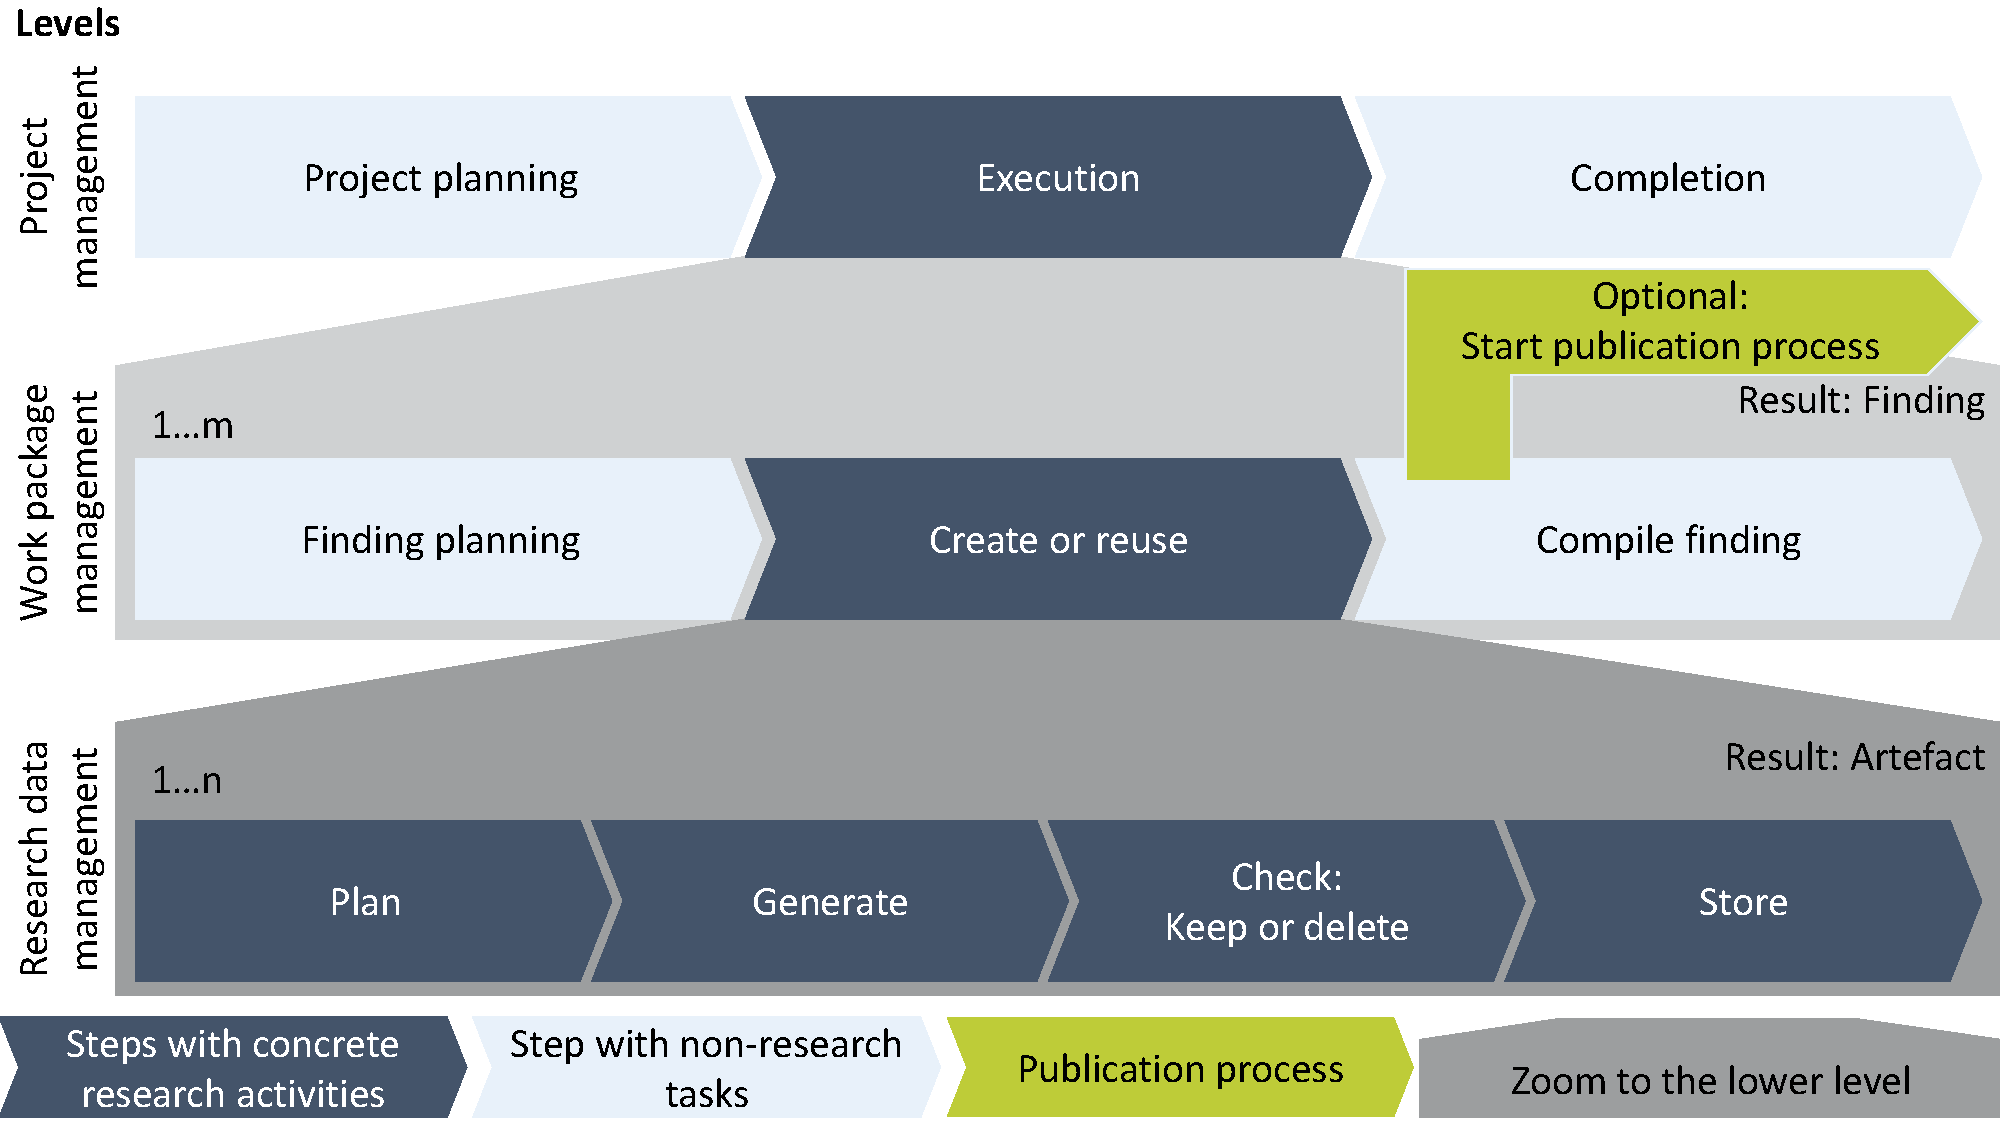
\includegraphics[trim={0 0.2cm 0cm 0cm}, clip, width=\textwidth]{figures/Levels_v2.pdf}
    \caption{General structure of the previously designed \hyperref[Glossary:research data management level]{\ac{rdm}} process \cite{Hamann.2024b}}
    \label{fig:Levels2}
\end{figure}

The \textbf{\ref{Glossary:project management level}} encompasses a waterfall-like approach.
The \ref{Glossary:project planning} includes all activities that happen before the research \ref{Glossary:project} is accepted, either in form of a provided grant or accepted \hyperref[Glossary:research proposal]{research proposal}.
Then the \ref{Glossary:project} is executed.
This \ref{Glossary:execution} includes the \ref{Glossary:content-wise execution}, \ref{Glossary:ongoing project management} and other activities.
The \ref{Glossary:project completion} starts when the \ref{Glossary:project} is coming to an end. 
It contains activities such as the writing of final reports or archiving of data.
This level of the process is depicted in greater detail in figure \ref{fig:Top_level}.

\begin{figure}[ht]
    \centering
    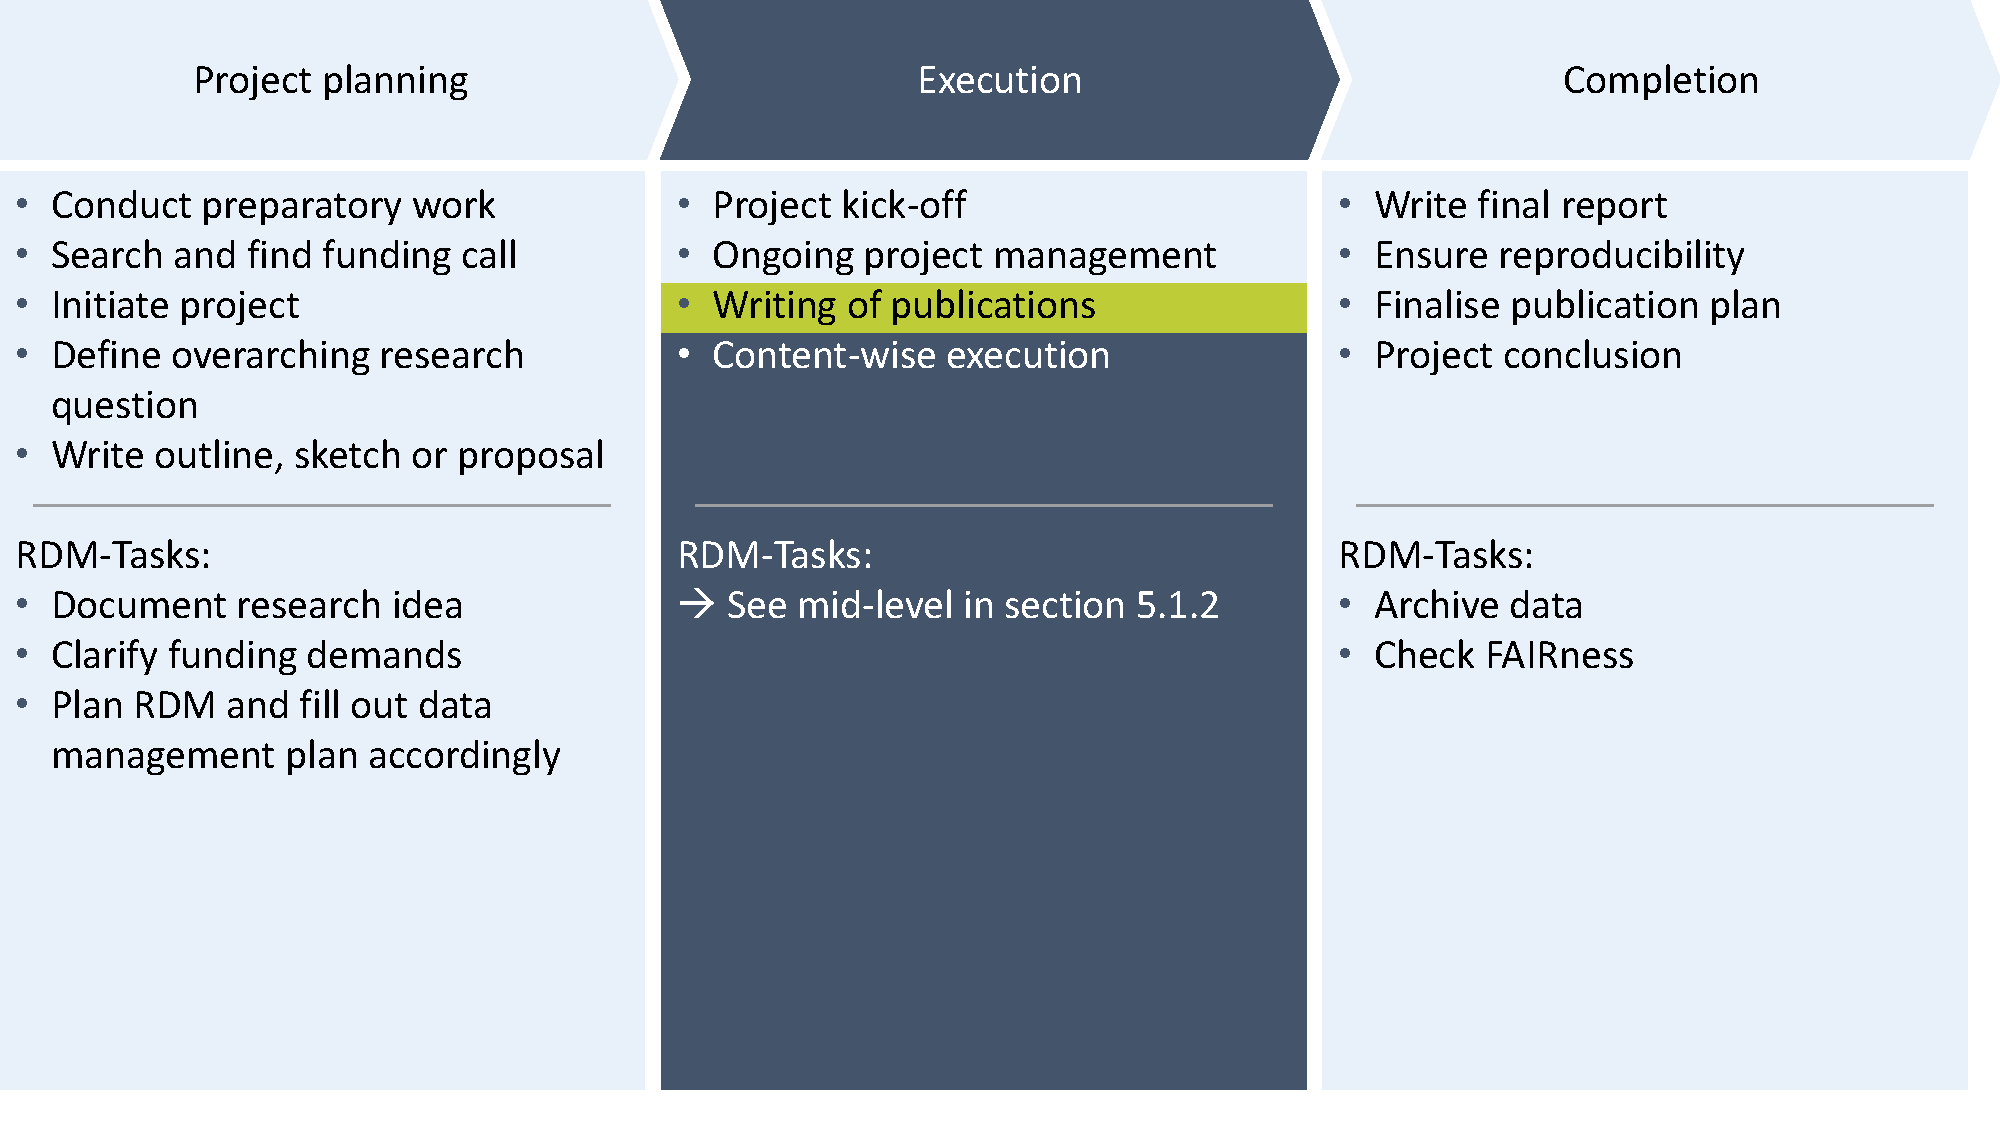
\includegraphics[trim={0 5.7cm 0cm 0cm}, clip, width=\textwidth]{figures/Top_level.pdf}
    \caption{Project management level of the proposed research process \cite{Hamann.2024b}}
    \label{fig:Top_level}
\end{figure}

Below the \ref{Glossary:project management level}, the \textbf{\ref{Glossary:work package level}} is placed, where work packages are processed.
Hence, this level is conducted \textit{n} times in an iterative approach.
For \ref{Glossary:finding planning}, firstly, a work package is chosen and divided into sub-steps needed to reach its goal. 
Afterwards, \ref{Glossary:artefact}s are created or reused - what researchers consider \enquote{actual research} and happens on the \ref{Glossary:research data management level}.
The creation of \ref{Glossary:artefact}s has to happen \textit{n} times to finish the work package.
Afterwards, the so created \ref{Glossary:artefact}s are compiled to a \ref{Glossary:finding} in the \ref{Glossary:finding compilation} step.
The \ref{Glossary:finding} is the result of the work package.
The work package management level is depicted in figure \ref{fig:Mid_level}.

\begin{figure}[ht]
    \centering
    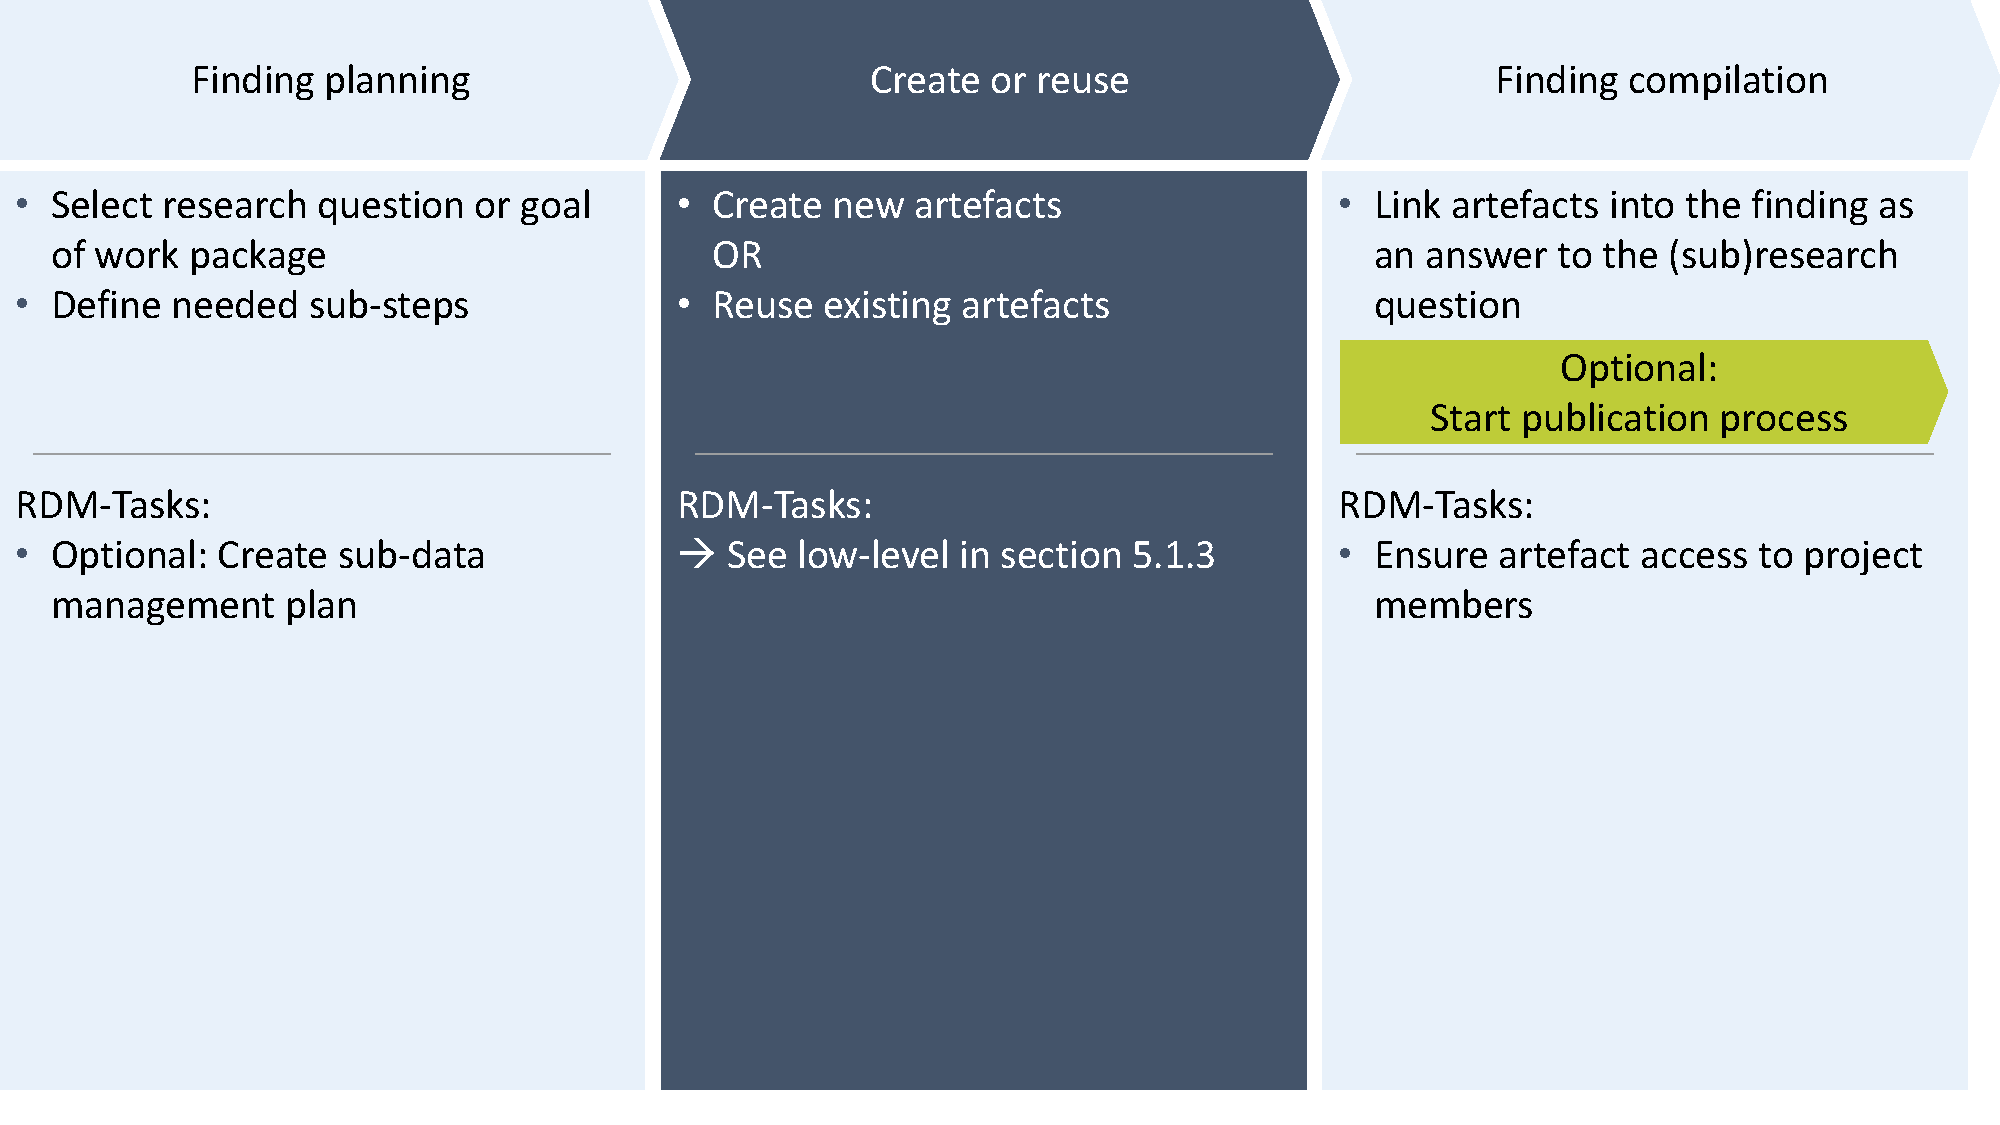
\includegraphics[trim={0 8.2cm 0cm 0cm}, clip, width=\textwidth]{figures/Mid_level.pdf}
    \caption{Work package management level of the proposed research process \cite{Hamann.2024b}}
    \label{fig:Mid_level}
\end{figure}

\hyperref[Glossary:artefact]{Artefact}s are the smallest unit of data in a research \ref{Glossary:project}.
Depending on the use case, it can be a single file, a data set of several files or physical object, e.g. a demonstrator or a workpiece.
If it is a digital piece of data, it is considered to be a digital object. \cite{Schwardmann.2020}
However, it is not necessarily a \ac{fairdo} by the definition of Schwardmann
\cite{Schwardmann.2020}, as a \ac{pid} might be missing.
An artefact can also be a real, physical object, as objects themselves can contain information that is stored within the object and can be analysed. \cite{Rixen.2026, Plomp.2021, Schilthuizen.2015}
%\todo{Digital Objects referenzieren}
An \ref{Glossary:artefact} is always the single outcome of one research method applied.

On the \textbf{research data management level}, each \ref{Glossary:artefact} is created by firstly planning its generation.
This planning happens immediately before it is \ref{Glossary:generate}d.
It is not a experimental design, rather the experimental design would be a previous \ref{Glossary:artefact}.
Instead, the \ref{Glossary:planning of the data generation} encompasses the gathering of the needed \ref{Glossary:artefact}, the methodical setup and the \ref{Glossary:check} if everything is properly configured.
%\todo{noch in weiterentwickelte grafik mit aufnehmen}
Then, the data is \ref{Glossary:generate}d.
Optimally, metadata is recorded along with the data generation, annotating the data, transferring it from data to data with context.
%\todo{wissenstreppe einbauen -> MR}
Afterwards, a \ref{Glossary:check} of the data \ref{Glossary:ensure}s the data was recorded at all, is reasonable and within expectations and not corrupted.
Otherwise, it can be deleted immediately.
If the data was recorded properly, it can be \ref{Glossary:store}d for further usage.
This process revolves around each \ref{Glossary:artefact}, as shown in figure \ref{fig:Artefact_n21} and in figure \ref{fig:Lowlevel}.


\begin{figure}[ht]
    \centering
    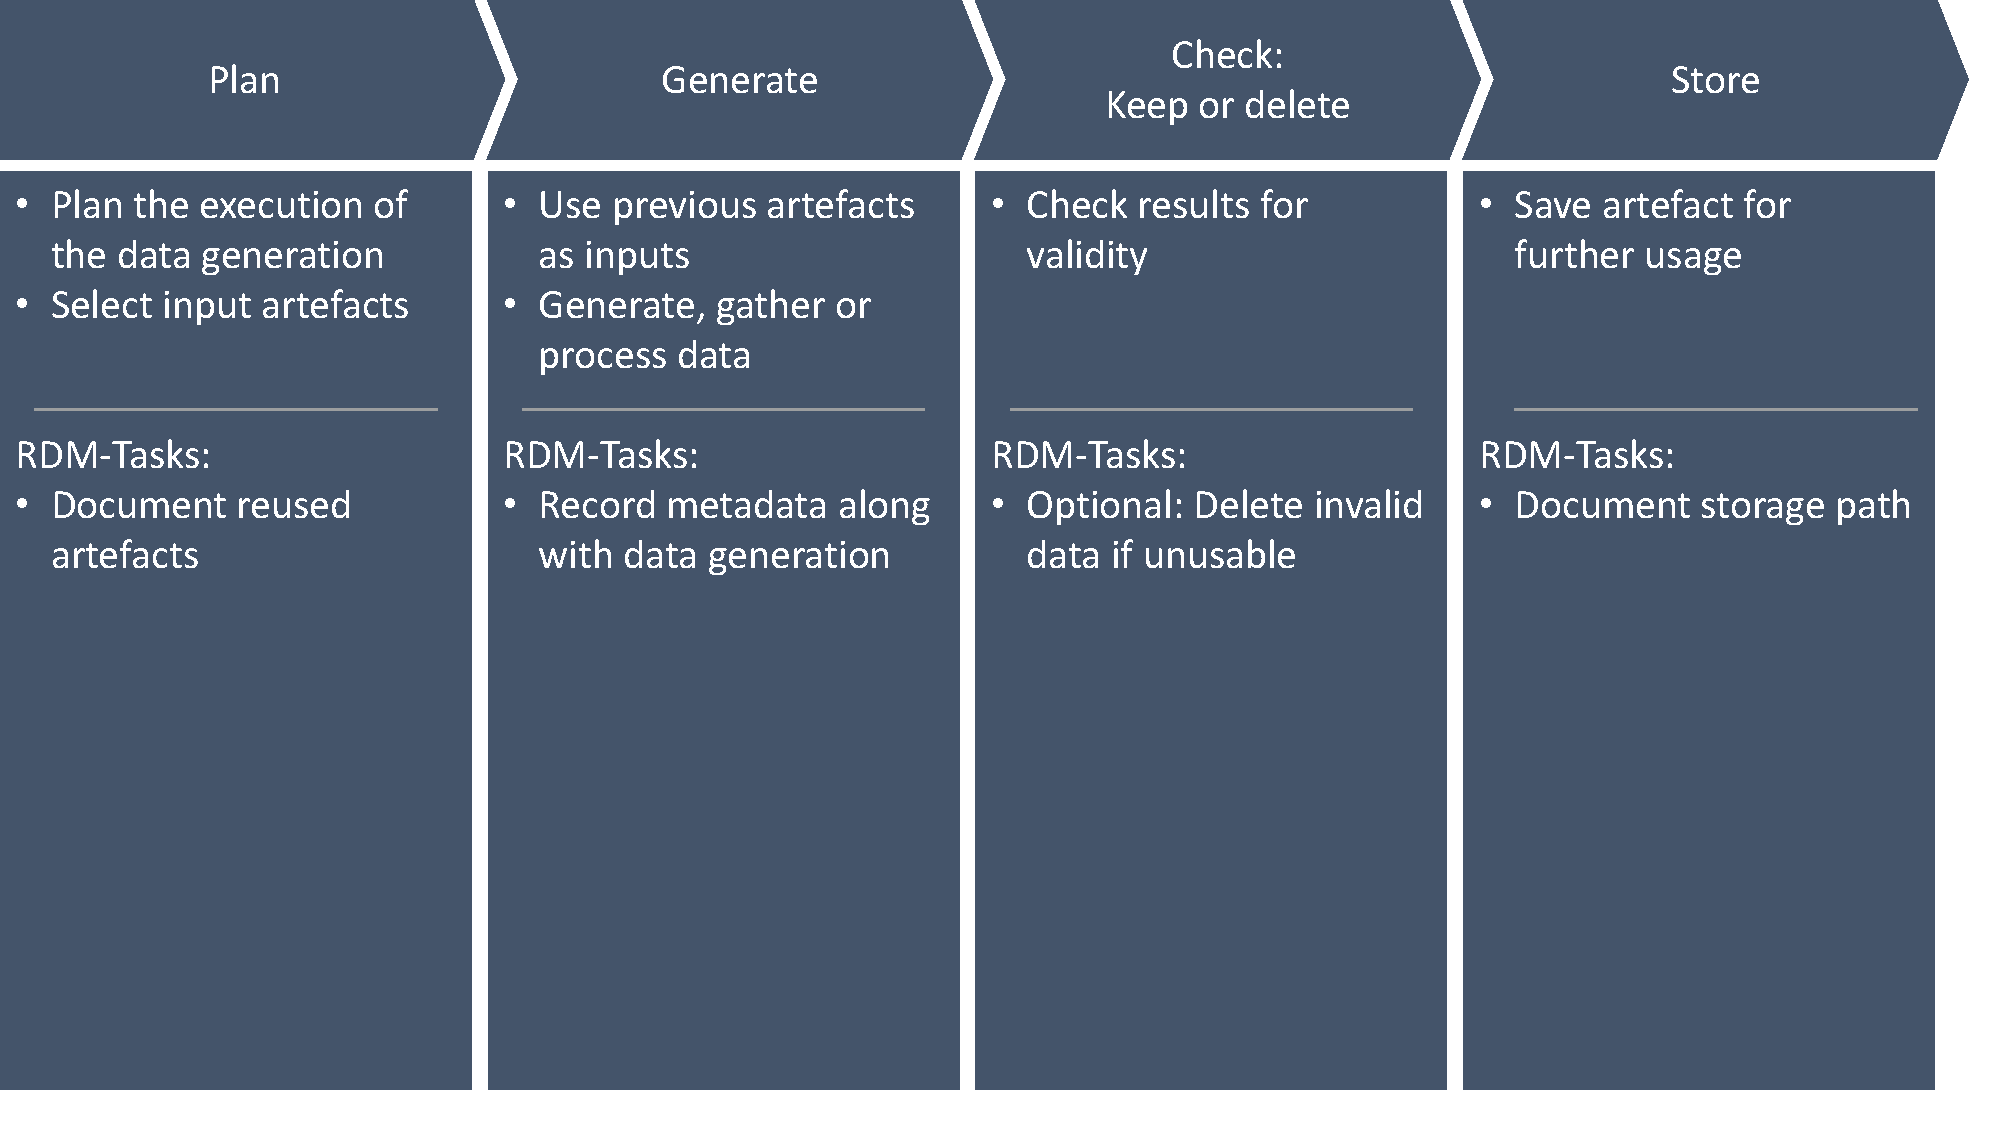
\includegraphics[trim={0 9cm 0 0cm}, clip, width=\textwidth]{figures/Low_level.pdf}
    \caption{Research data management level of the proposed research process \cite{Hamann.2024b}}
    \label{fig:Lowlevel}
\end{figure}


Additionally to the \ref{Glossary:finding compilation}, a \textbf{\ref{Glossary:publication process}} can be started. It starts optionally from the \ref{Glossary:work package level} and runs in parallel. The \ref{Glossary:topic} definition, the first step in the process, is determined by the \ref{Glossary:finding compilation}. The \ref{Glossary:publication} is then prepared, which includes, for example, finding a suitable medium. This is followed by \ref{Glossary:editing}: \hyperref[Glossary:artefact]{Artefact}s, \ref{Glossary:finding}s and the knowledge generated as a result are converted into text and - as an RDM task - published. In the \ref{Glossary:submission} step, the \ref{Glossary:publication} is submitted, subjected to a quality check through a peer review process and finally published. This is at last followed by \ref{Glossary:dissemination} as illustrated in figure \ref{fig:Publication}.

\begin{figure}[ht]
    \centering
    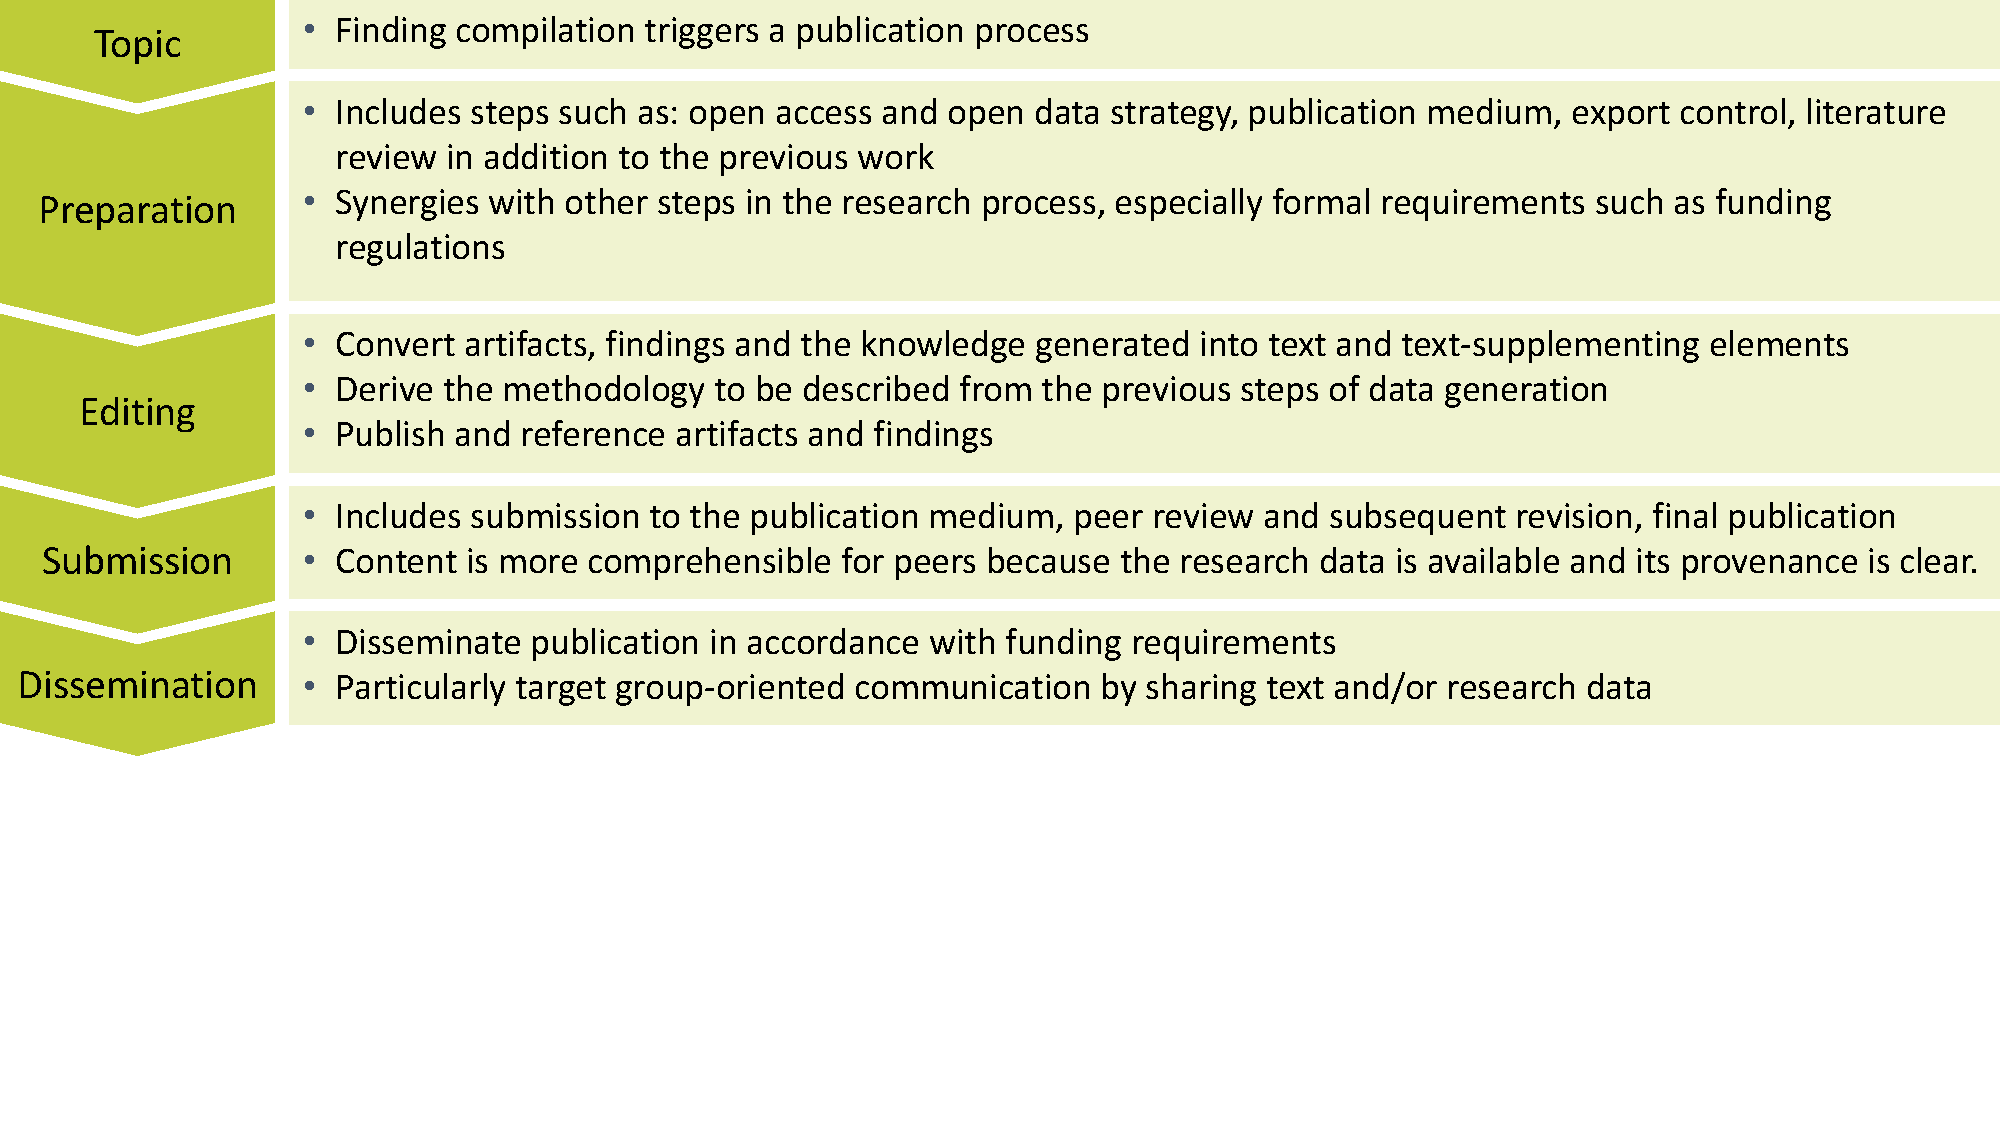
\includegraphics[trim={0 6cm 0 0}, clip, width=\textwidth]{figures/Publication_condensed.pdf}
    \caption{The publication process \cite{Hamann.2024b}}
    \label{fig:Publication}
\end{figure}

The goal of the developed process is the combination of \ref{Glossary:project}-oriented research, demands of engineering researchers and \hyperref[Glossary:research data management level]{\ac{rdm}} processes.
This combination could solve the problem of lacking applicability of \hyperref[Glossary:research data management level]{\ac{rdm}} found in \cite{Hamann.2024b}.
However, it has to be validated, if this goal could be reached by the proposed process.

Parts of the proposed process has also already been taken up and further investigated and implemented by Wawer et al. \cite{Wawer.2024}.
However, in their paper, Wawer et al. \cite{Wawer.2024} focus on the \ref{Glossary:research data management level}, elaborating on the concept of \ref{Glossary:artefact}s, their linking and compilation into a research result.
In addition to their process, Wawer et al. \cite{Wawer.2024} point out, \enquote{the context of RDM should be established at \ref{Glossary:project level}, as data is usually archived at the end of the project and a data management plan is created at the start of the project}.
This establishment is the focus of our proposed process both in this and the previous paper.
Yet, to this point the process has not been proven to be sufficient, which makes a validation of this process necessary as presented in the next section.

\begin{comment}

\begin{figure}[ht]
    \centering
    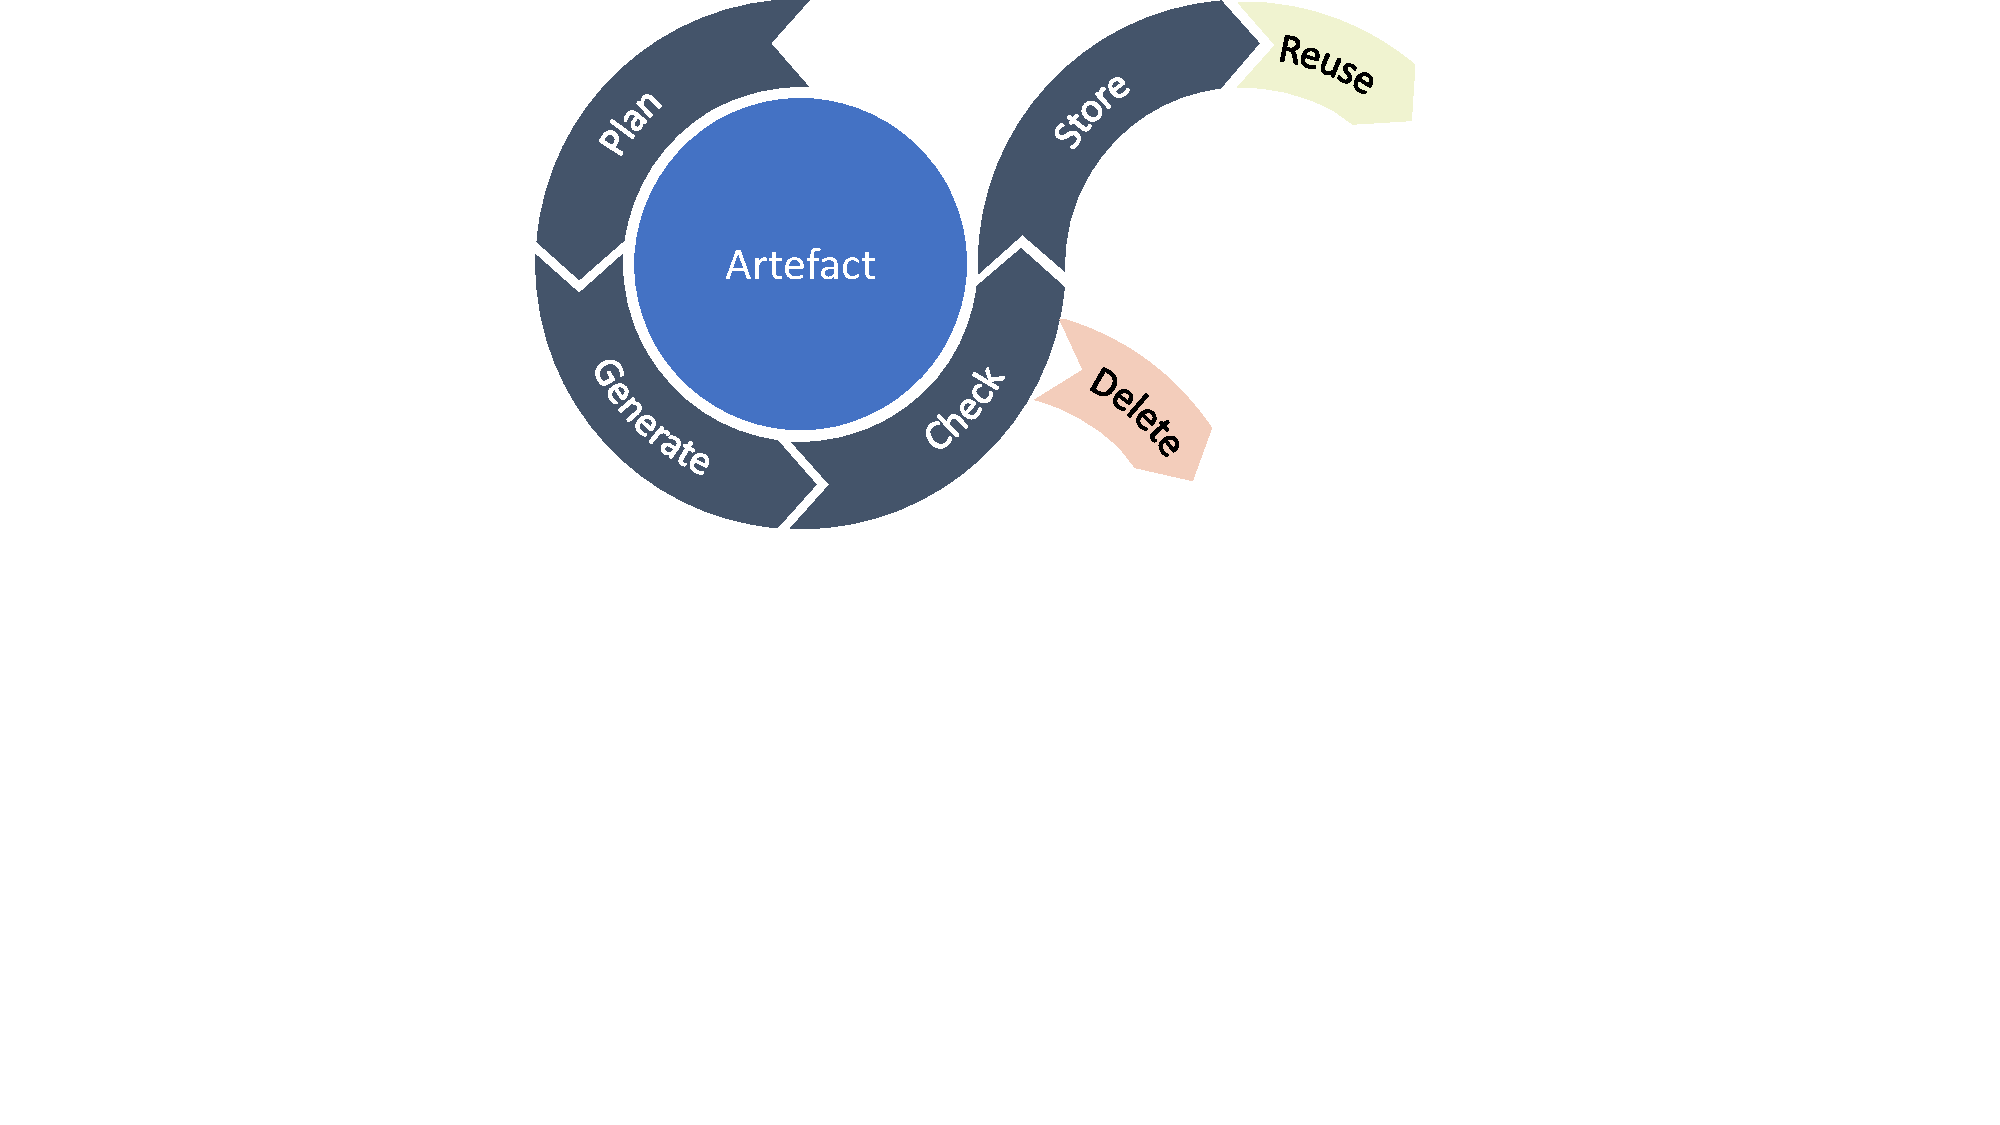
\includegraphics[trim={0cm 10cm 0cm 0cm}, clip, width=\textwidth]{figures/Artefact.pdf}
    \caption{Procedure of \ref{Glossary:artefact} generation as a new form of \ac{dlc}}
    \label{fig:Artefact}
\end{figure}

\begin{figure}[ht]
    \centering
    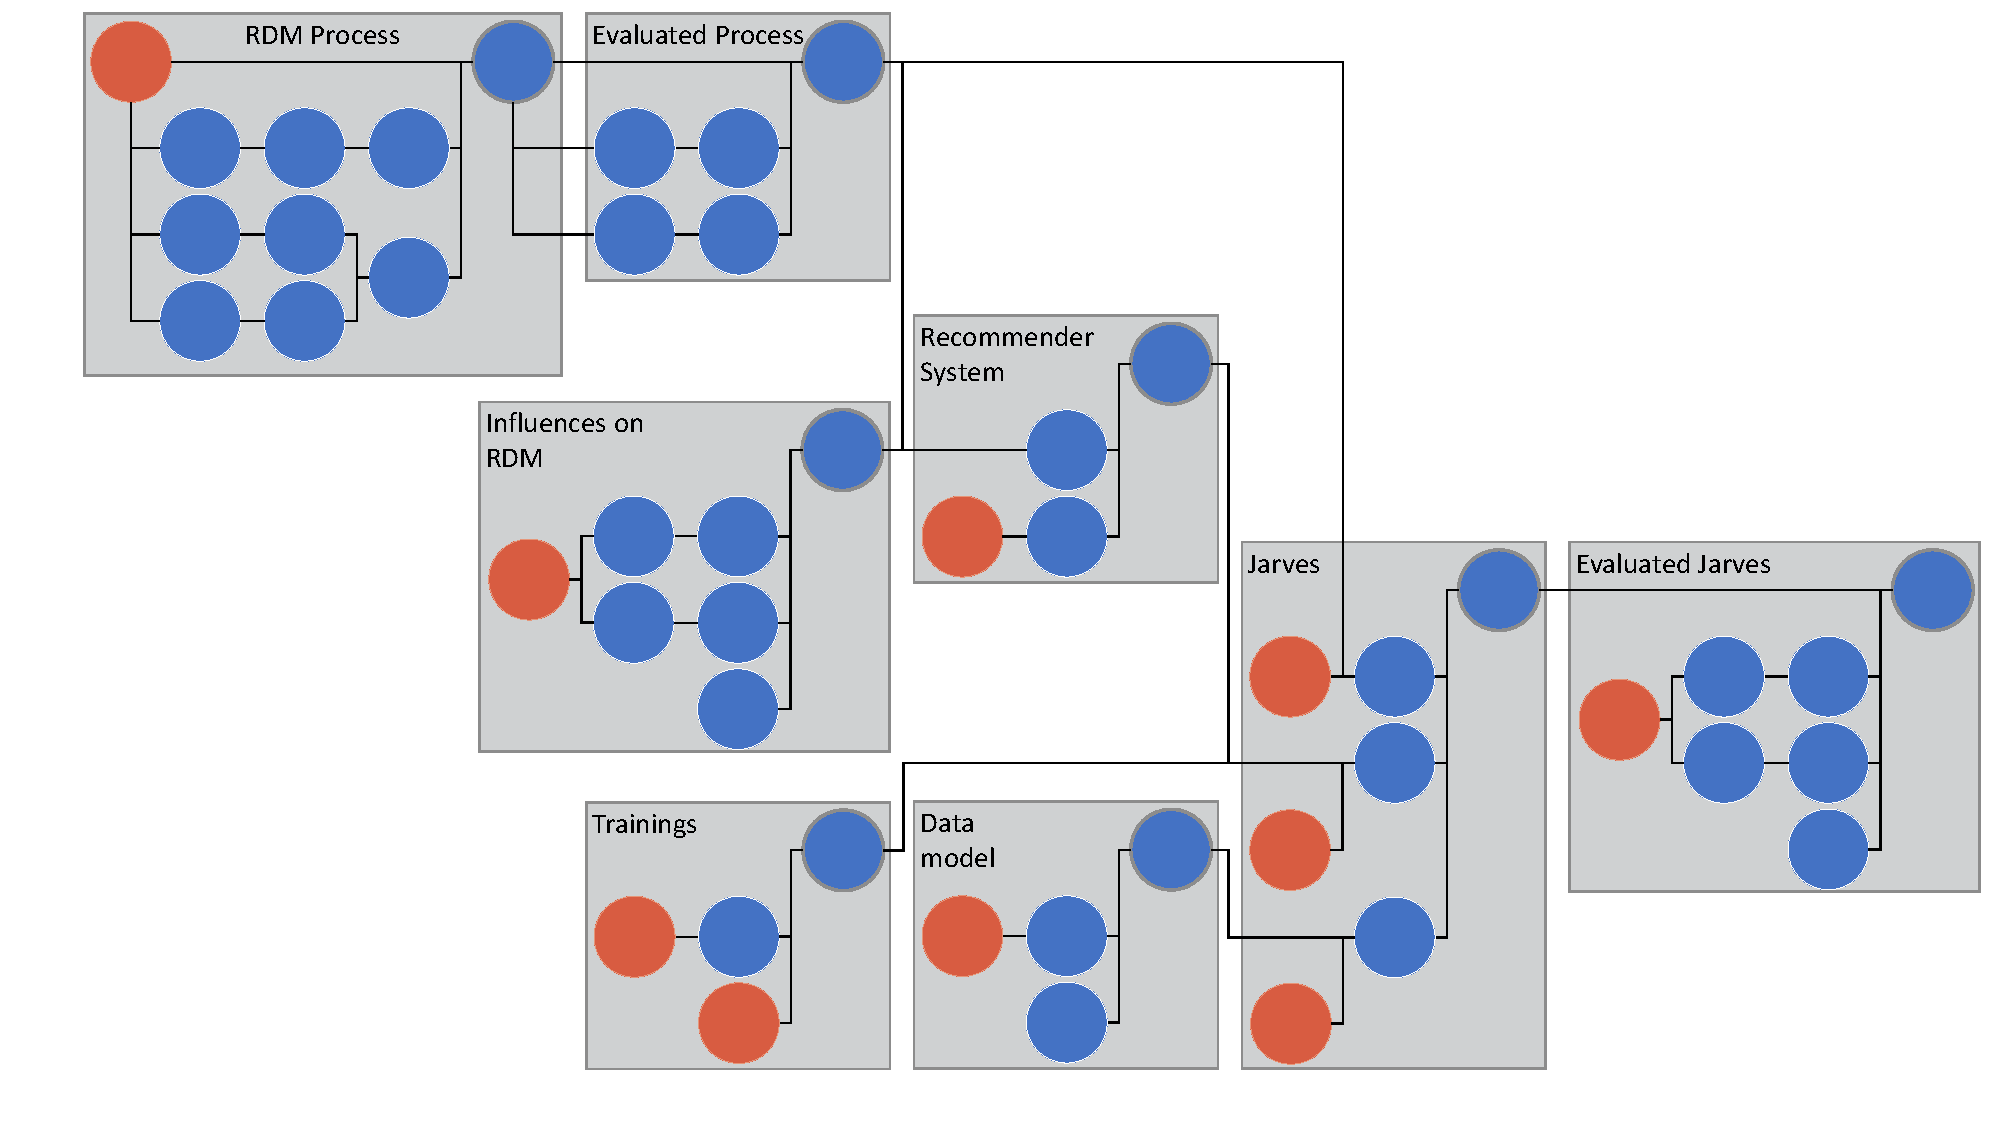
\includegraphics[trim={0cm 0cm 0cm 0cm}, clip, width=\textwidth]{figures/Jarves_Project_View.pdf}
    \caption{An example of the \ref{Glossary:research project} Jarves}
    \label{fig:Jarves_Project_View}
\end{figure}


\end{comment}

\subsection{Tables on Codes}
\label{tablestofigures}

This section of the appendix further elaborates on the exact numbers of codes gathered for each of the processes parts.
Table \ref{tab:DescriptiveFeedback_top} shows codes gathered for the project management level.

\begin{table}[ht]
    \begin{tabularx}{\textwidth}{l|X|X|X||X}
        % \toprule
        \textbf{Code Group} & \textbf{Acceptance} & \textbf{Rejection} & \textbf{Indifference} & \textbf{Total group sum}  \\
        \toprule
        \makecell[l]{Project management level\\(total)}  & 92 & 40 & 11 & 143 \\
        \midrule
        \midrule
        Comprised of: &  &  &  &  \\
        \, General & \, 17 & \, 7 & \, 5 & \, 29 \\
        \, Project planning & \, 30 & \, 13 & \, 5  & \, 48 \\
        \, Execution & \, 37 & \, 8  & \, 1 & \, 46 \\
        \, Completion & \, 8 & \, 12 & \, 0 & \, 20 \\
        % \hline \hline
        % &&            Sum: & \\
    \end{tabularx}
    \caption{Codes on the feedback received on the project management level}
    \label{tab:DescriptiveFeedback_top}
\end{table}

Table \ref{tab:DescriptiveFeedback_mid} depicts the number of codes on the feedback received on the work package management level.


\begin{table}[ht]
    \begin{tabularx}{\textwidth}{l|X|X|X||X}
        % \toprule
        \textbf{Code Group} & \textbf{Acceptance} & \textbf{Rejection} & \textbf{Indifference} & \textbf{Total group sum}  \\
        \toprule
        \makecell[l]{Work package management\\level (total)} & 74 & 22 & 8 & 104 \\
        \midrule
        \midrule
        Comprised of: &  &  &  &  \\
        \, General & \, 28 & \, 5 & \, 5 & \, 38 \\
        \, Finding planning & \, 13 & \, 5 & \, 0 & \, 18 \\
        \, Create or Reuse & \, 22 & \, 2 & \, 2 & \,  26\\
        \, Finding compilation & \, 11 & \, 10 & \, 1 & \, 22 \\
        % \hline \hline
        % &&            Sum: & \\
    \end{tabularx}
    \caption{Codes on the feedback received on the work package management level}
    \label{tab:DescriptiveFeedback_mid}
\end{table}


Table \ref{tab:DescriptiveFeedback_low} depicts the number of codes on the feedback received on the research data management level.

\begin{table}[ht]
    \begin{tabularx}{\textwidth}{l|X|X|X||X}
        % \toprule
        \textbf{Code Group} & \textbf{Acceptance} & \textbf{Rejection} & \textbf{Indifference} & \textbf{Total group sum}  \\
        \toprule
        \makecell[l]{Research data management level\\(total)} & 73 & 28 & 10 & 111 \\
        \midrule
        \midrule
        Comprised of: &  &  &  &  \\
        \, General & \, 33 & \, 6 & \, 7  & \, 46 \\
        \, Plan & \, 8 & \, 7 & \, 2 & \, 17 \\
        \, Generate & \, 10 & \, 2 & \, 1 & \, 13 \\
        \, Check & \, 19 & \, 12 & \, 0 & \, 31 \\
        \, Store & \, 3 & \, 1 & \, 0 & \, 4 \\
        % \hline \hline
        % &&            Sum: & \\
    \end{tabularx}
    \caption{Codes on the feedback received on the research data management level}
    \label{tab:DescriptiveFeedback_low}
\end{table}


Table \ref{tab:DescriptiveFeedback_pub} depicts the number of codes on the feedback received on the publication workflow.

\begin{table}[ht]
    \begin{tabularx}{\textwidth}{l|X|X|X||X}
        % \toprule
        \textbf{Code Group} & \textbf{Acceptance} & \textbf{Rejection} & \textbf{Indifference} & \textbf{Total group sum}  \\
        \toprule
        \makecell[l]{Publication workflow (total)}  & 55 & 46 & 31 & 132 \\
        \midrule
        \midrule
        Comprised of: &  &  &  &  \\
        \, General & \, 10 & \, 11 & \, 25 & \, 46 \\
        \, Topic & \, 11  & \, 13 & \, 2 & \, 26 \\
        \, Preparation & \, 12 & \, 6 & \, 1 & \, 19 \\
        \, Editing & \, 12 & \, 8 & \, 2 & \, 22 \\
        \, Submission & \, 8 & \, 7 & \, 1 & \, 16 \\
        \, Dissemination & \, 2 & \, 1 & \, 0 & \, 3 \\
        % \hline \hline
        % &&            Sum: & \\
    \end{tabularx}
    \caption{Codes on the feedback received on the publication workflow}
    \label{tab:DescriptiveFeedback_pub}
\end{table}

%
% Acknowledgements, contributions & roles, and references
% will be set automatically at the end of the document
%
%
\end{document}
